\باب{جزوی تفرقی مساوات}
مختلف طبعی اور جیومیٹریائی مسائل جہاں دو یا دو سے زیادہ متغیرات پر مبنی تفاعل پایا جاتے ہوں، جزوی تفرقی مساوات کو جنم دیتے ہیں۔یہ متغیرات وقت اور خلا کے محدد ہو سکتے ہیں۔اس باب میں انجینئری نقطہ نظر سے اہم مسائل پر غور کیا جائے گا۔ان مساوات کو طبعی نظام کی نمونہ کے طور پر حاصل کرنے کے بعد ابتدائی قیمت اور سرحدی قیمت مسائل حل کرنے کی تراکیب پر غور کیا جائے گا، یعنی ان مساوات کو دی گئی طبعی شرائط کے مطابق حل کیا جائے گا۔

ہم دیکھیں گے کہ جزوی تفرقی مساوات کو لاپلاس بدل کی مدد سے حل کیا جا سکتا ہے۔

\حصہ{بنیادی تصورات}
دو یا دو سے زیادہ غیر تابع متغیرات کی نا معلوم تفاعل اور اس کی ایک یا ایک سے زیادہ تفرقات پر مبنی مساوات کو \اصطلاح{جزوی تفرقی مساوات}\فرہنگ{تفرقی!جزوی مساوات}\فرہنگ{جزوی!تفرقی مساوات}\حاشیہب{partial differential equation}\فرہنگ{differential!partial equation} کہتے ہیں۔ بلند تر تفرق کا درجہ مساوت کا \اصطلاح{درجہ}\فرہنگ{درجہ!جزوی تفرقی مساوات}\فرہنگ{جزوی!درجہ مساوات}\حاشیہب{order}\فرہنگ{order!partial differential equation} کہلاتا ہے۔ 

سادہ تفرقی مساوات کی طرح اگر جزوی تفرقی مساوات میں تابع متغیر (نا معلوم تفاعل) اور اس کے تفرق کی طاقت اکائی ہو تب  یہ تفرقی مساوات \اصطلاح{خطی}\فرہنگ{خطی}\حاشیہب{linear}\فرہنگ{linear} کہلائے گی۔اگر مساوات کا ہر رکن، تابع متغیرہ یا تابع متغیرہ کی تفرقات میں سے کوئی ایک تفرق ہو تب اس کو \اصطلاح{ہم جنسی}\فرہنگ{ہم جنسی!جزوی تفرقی مساوات}\حاشیہب{homogeneous}\فرہنگ{homogeneous!partial differential equation} کہیں گے ورنہ یہ \اصطلاح{غیر ہم جنسی}\فرہنگ{غیر ہم جنسی!جزوی تفرقی مساوات}\حاشیہب{non homogeneous}\فرہنگ{non homogeneous!partial differential equation} کہلائے گی۔   

%===============
\ابتدا{مثال}\quad اہم خطی دو درجی جزوی تفرقی مساوات\\
\begin{align}
&\frac{\partial^{\,2}u}{\partial t^2}=c^2\frac{\partial^{\,2}u}{\partial x^2}\label{مساوات_جزوی_الف}\quad \quad 
\text{\RL{یک بعدی مساوات موج}}\\
&\frac{\partial u}{\partial t}=c\frac{\partial^{\,2}u}{\partial x^2}\label{مساوات_جزوی_ب}\quad \quad \text{\RL{یک بعدی مساوات حرارت}}\\
&\frac{\partial^{\,2}u}{\partial x^2}+\frac{\partial^{\,2}u}{\partial y^2}=0\label{مساوات_جزوی_پ}\quad \quad \quad 
\text{\RL{دو بعدی لاپلاس مساوات}}\\
&\frac{\partial^{\,2}u}{\partial x^2}+\frac{\partial^{\,2}u}{\partial y^2}=f(x,y)\label{مساوات_جزوی_ت}\quad \quad \quad \text{\RL{دو بعدی پوئسن مساوات}}\\
&\frac{\partial^{\,2}u}{\partial x^2}+\frac{\partial^{\,2}u}{\partial y^2}+\frac{\partial^{\,2}u}{\partial z^2}=0\label{مساوات_جزوی_ٹ}\quad \quad \quad \text{\RL{تین بعدی لاپلاس مساوات}}
\end{align}
یہاں \عددی{c} مستقل ہے، \عددی{t} وقت کو ظاہر کرتی ہے جبکہ \عددی{x}، \عددی{y}، \عددی{z} کارتیسی محدد ہیں۔مساوات \حوالہ{مساوات_جزوی_ت} میں اگر \عددی{f(x,y)\ne 0} ہو تب یہ غیر ہم جنسی ہو گی۔باقی تمام مساوات ہم جنسی ہیں۔
\انتہا{مثال}
%===========================

فضا میں غیر تابع متغیرہ کی کسی خطہ  \عددی{R} میں جزوی تفرقی مساوات کے \اصطلاح{حل} سے مراد ایسا تفاعل ہے جو خود اور جس کے وہ تمام تفرقات جو اس مساوات میں پائے جاتے ہوں کسی ایسے خطے میں موجود ہوں  جس کا \عددی{R} حصہ ہو اور یہ تمام مل کر پورے خطہ \عددی{R} میں اس مساوات کو مطمئن کرتے ہوں۔(عموماً \عددی{R} کی سرحد پر اس تفاعل کا استمراری ہونا اور درکار تفرقات کا خطہ کے اندرون معین ہونے کے ساتھ ساتھ خطہ کے اندرون مساوات کو مطمئن کرنا درکار ہو گا۔)

عموماً جزوی تفرقی مساوات کے تمام حل کی تعداد بہت زیادہ ہو گی۔ مثلاً جیسا آپ تصدیق کر سکتے ہیں کہ تفاعل
\begin{align}\label{مساوات_جزوی_مثال_تفاعل}
u=x^2-y^2,\quad u=e^x\cos y,\quad u=\ln(x^2+y^2)
\end{align} 
جو ایک دوسرے سے بالکل مختلف ہیں مساوات \حوالہ{مساوات_جزوی_پ} کے حل ہیں۔ہم بعد میں دیکھیں گے کہ جزوی تفرقی مساوات کا یکتا حل حاصل کرنے کی خاطر مزید معلومات درکار ہو گی جو طبعی حالت سے حاصل ہو گی۔مثال کے طور پر کبھی کبھار سرحد کے کسی حصے پر درکار حل کی قیمت معلوم ہو گی (\اصطلاح{سرحدی شرائط}\فرہنگ{سرحدی شرائط}\حاشیہب{boundary conditions}\فرہنگ{boundary conditions}) جب کہ بعض اوقات ابتدائی لمحہ \عددی{t=0} پر حل کی قیمت معلوم ہو گی (\اصطلاح{ابتدائی شرائط}\فرہنگ{ابتدائی شرائط}\حاشیہب{initial conditions}\فرہنگ{initial conditions})۔ 

ہم جانتے ہیں کہ اگر سادہ تفرقی مساوات خطی اور ہم جنسی ہو تب اس کی معلوم حل سے مزید حل بذریعہ خطی میل حاصل کیے جا سکتے ہیں۔ جزوی تفرقی مساوات کے لئے بھی ایسا کرنا ممکن ہے جیسا درج ذیل مسئلہ کہتا ہے۔

%=========================
\ابتدا{مسئلہ}\شناخت{مسئلہ_جزوی_بنیادی}\quad بنیادی مسئلہ\\
اگر کسی خطہ \عددی{R} میں  خطی ہم جنسی جزوی تفرقی مساوات کے دو حل \عددی{u_1} اور \عددی{u_2} ہوں تب
\begin{align*}
u=c_1u_1+c_2u_2
\end{align*} 
جہاں \عددی{c_1} اور \عددی{c_2} کوئی مستقل ہیں، بھی اس خطے میں اس مساوات کا حل ہو گا۔
\انتہا{مسئلہ}
%====================

اس مسئلے کا ثبوت نہایت آسان اور مسئلہ \حوالہ{مسئلہ_دو_درجی_خطی_میل} کی ثبوت سے ملتا جلتا ہے لہٰذا یہ آپ پر چھوڑا جاتا ہے۔

%================
\حصہء{سوالات}

%==================
\ابتدا{سوال}\quad
مسئلہ \حوالہ{مسئلہ_جزوی_بنیادی} کو دو اور تین متغیرات کی دو درجی جزوی تفرقی مساوات کے لئے ثابت کریں۔
\انتہا{سوال}
%======================
\ابتدا{سوال}\quad تصدیق کریں کہ مساوات \حوالہ{مساوات_جزوی_مثال_تفاعل} میں دیے گئے تمام تفاعل مساوات \حوالہ{مساوات_جزوی_پ} کے حل ہیں۔\\
جواب:\quad \عددی{u=x^2+y^2} لیتے ہیں۔ یوں \عددی{\tfrac{\partial^{\,2}u}{\partial x^2}=2} اور \عددی{\tfrac{\partial^{\,2}u}{\partial y^2}=2} ہو گا۔انہیں مساوت \حوالہ{مساوات_جزوی_پ} میں پر کرتے ہوئے \عددی{0=0} ملتا ہے۔یوں \عددی{u} تفرقی مساوات کو مطمئن کرتا ہے۔
\انتہا{سوال}
%====================
سوال \حوالہ{سوال_جزوی_لاپلاس_مطمئن_الف} تا سوال \حوالہ{سوال_جزوی_لاپلاس_مطمئن_ب} میں تصدیق کریں کہ دیا گیا تفاعل لاپلاس مساوات کو مطمئن کرتا ہے۔

%==================
\ابتدا{سوال}\شناخت{سوال_جزوی_لاپلاس_مطمئن_الف} \quad
$u=2xy$
\انتہا{سوال}
%=====================
\ابتدا{سوال} \quad
$u=e^x\sin y$
\انتہا{سوال}
%=====================
\ابتدا{سوال} \quad
$u=\tan^{-1}\frac{y}{x}$
\انتہا{سوال}
%=====================
\ابتدا{سوال} \quad
$u=x^3-3xy^2$
\انتہا{سوال}
%=====================
\ابتدا{سوال} \quad
$u=\sin x\sinh y$
\انتہا{سوال}
%=====================
\ابتدا{سوال}\شناخت{سوال_جزوی_لاپلاس_مطمئن_ب} \quad
$u=x^4-6x^2y^2+y^4$
\انتہا{سوال}
%=====================
سوال \حوالہ{سوال_جزوی_حراری_مطمئن_الف} تا سوال \حوالہ{سوال_جزوی_حراری_مطمئن_ب} میں تصدیق کریں کہ دیا گیا تفاعل حراری مساوات \حوالہ{مساوات_جزوی_ب} کو مطمئن کرتا ہے۔

%==================
\ابتدا{سوال}\شناخت{سوال_جزوی_حراری_مطمئن_الف} \quad
$u=e^{-2t}\cos x$
\انتہا{سوال}
%======================
\ابتدا{سوال}\quad
$u=e^{-t}\sin 3x$
\انتہا{سوال}
%======================
\ابتدا{سوال}\شناخت{سوال_جزوی_حراری_مطمئن_ب}\quad
$u=e^{-4t}\cos \omega x$
\انتہا{سوال}
%======================
سوال \حوالہ{سوال_جزوی_موج_مطمئن_الف} تا سوال \حوالہ{سوال_جزوی_موج_مطمئن_ب} میں تصدیق کریں کہ دیا گیا تفاعل موج کی مساوات \حوالہ{مساوات_جزوی_الف} کو مطمئن کرتا ہے۔

%==================
\ابتدا{سوال}\شناخت{سوال_جزوی_موج_مطمئن_الف}\quad
$u=x^2+4t^2$
\انتہا{سوال}
%======================
\ابتدا{سوال}\quad
$u=x^3+3xt^2$
\انتہا{سوال}
%======================
\ابتدا{سوال}\شناخت{سوال_جزوی_موج_مطمئن_ب}\quad
$u=\sin \omega ct\sin \omega x$
\انتہا{سوال}
%======================
\ابتدا{سوال}\quad
تصدیق کریں کہ 
$u=\sqrt{x^2+y^2+z^2}$
تین بعدی لاپلاس مساوات \حوالہ{مساوات_جزوی_ٹ} کو مطمئن کرتا ہے۔
\انتہا{سوال}
%========================
\ابتدا{سوال}\quad
تصدیق کریں کہ
$u(x,y)=a\ln(x^2+y^2)+b$
دو بعدی لاپلاس مساوات \حوالہ{مساوات_جزوی_پ} کا حل ہے۔دی گئی سرحدی شرائط کے تحت دائرہ \عددی{x^2+y^2=1} پر  \عددی{u=0} اور دائرہ \عددی{x^2+y^2=9} پر \عددی{u=5} ہے۔مستقل \عددی{a} اور \عددی{b} کی ایسی قیمتیں دریافت کریں کہ \عددی{u} ان سرحدی شرائط کو مطمئن کرے۔حاصل \عددی{u} کی ترسیم کھینچیں۔
\انتہا{سوال}
%======================
\ابتدا{سوال}\quad
تصدیق کریں کہ
$u(x,t)=v(x+ct)+w(x-ct)$
موج کی مساوات \حوالہ{مساوات_جزوی_الف} کو مطمئن کرتا ہے۔یہاں \عددی{u} اور \عددی{v} دو مرتبہ قابل تفرق تفاعل ہیں۔
\انتہا{سوال}
%====================
اگر جزوی تفرقی مساوات میں صرف ایک متغیر کے ساتھ تفرقات پائے جاتے ہوں تب اس کو سادہ تفرقی مساوات تصور کر کے حل کیا جا سکتا ہے جہاں باقی متغیرات کو مستقل تصور کیا جاتا ہے۔سوال \حوالہ{سوال_جزوی_سادہ_الف} تا سوال \حوالہ{سوال_جزوی_سادہ_ب} کو حل کریں جہاں \عددی{u} کے متغیرات \عددی{x} اور \عددی{y} ہیں۔

%====================
\ابتدا{سوال}\شناخت{سوال_جزوی_سادہ_الف}\quad
$u_{xx}-u=0$\\
جواب:\quad
$u=c_1(y)e^x+c_2(y)e^{-x}$
\انتہا{سوال}
%====================
\ابتدا{سوال}\quad
$u_{y}+yu=0$\\
جواب:\quad
$u=c(x)e^{-\tfrac{y^2}{2}}$
\انتہا{سوال}
%====================
\ابتدا{سوال}\quad
$u_{yy}+9u=0$\\
جواب:\quad
$u=c_1(y)\cos 3x+c_2(y)\sin 3x$
\انتہا{سوال}
%====================
\ابتدا{سوال}\شناخت{سوال_جزوی_سادہ_ب}\quad
$u_x+2xyu=0$\\
جواب:\quad
$u=c(y)e^{-x^2y}$
\انتہا{سوال}
%====================
سوال \حوالہ{سوال_جزوی_تلاش_الف} تا سوال \حوالہ{سوال_جزوی_تلاش_ب} میں \عددی{u_x=p} لیتے ہوئے حل تلاش کریں۔

%================
\ابتدا{سوال}\شناخت{سوال_جزوی_تلاش_الف}\quad
$u_{xy}=0$\\
جواب:\quad
$u=v(x)+w(y)$
\انتہا{سوال}
%======================
\ابتدا{سوال}\quad
$u_{xy}=u_x$
\انتہا{سوال}
%=======================
\ابتدا{سوال}\quad
$u_{xy}+u_x=0$\\
جواب:\quad
$u=v(x)e^{-y}+w(y)$
\انتہا{سوال}
%=======================
\ابتدا{سوال}\شناخت{سوال_جزوی_تلاش_ب}\quad
$u_{xy}+u_x+x+y+1=0$
\انتہا{سوال}
%=======================
سوال \حوالہ{سوال_جزوی_نظام_الف} تا سوال \حوالہ{سوال_جزوی_نظام_ب} میں دیے گئے تفرقی مساوات کی نظام کے حل تلاش کریں۔ 

%=================
\ابتدا{سوال}\شناخت{سوال_جزوی_نظام_الف}\quad
$u_{xx}=0,\quad u_{yy}=0$\\
جواب:\quad
$u=axy+bx+cy+k$
\انتہا{سوال}
%==================
\ابتدا{سوال}\quad
$u_{x}=0,\quad u_{y}=0$
\انتہا{سوال}
%==================
\ابتدا{سوال}\quad
$u_{xx}=0,\quad u_{xy}=0$\\
جواب:\quad
$u=cx+g(y)$
\انتہا{سوال}
%==================
\ابتدا{سوال}\شناخت{سوال_جزوی_نظام_ب}\quad
$u_{xx}=0,\quad u_{xy}=0,\quad u_{yy}=0$
\انتہا{سوال}
%==================
\ابتدا{سوال}\quad
تصدیق کریں کہ اگر سطح \عددی{z=z(x,y)} پر منحنی \عددی{z=c} محور \عددی{x} کے متوازی سیدھے خطوط ہوں، جہاں \عددی{c} مستقل ہے، تب \عددی{z} تفرقی مساوات \عددی{z_x=0} کا حل ہو گا۔ایسی ایک مثال بھی پیش کریں۔  
\انتہا{سوال}
%=====================
\ابتدا{سوال}\quad
تصدیق کریں کہ \عددی{yz_x-xz_y=0} کا حل \عددی{z=z(x,y)} سطح گردش ہے۔اس کی مثال پیش کریں۔ (اشارہ: \عددی{x=r\cos \theta} اور \عددی{y=r\sin \theta} لے کر تفرقی مساوات کو \عددی{z_{\theta}=0} میں تبدیل کریں۔)
\انتہا{سوال}
%======================

\حصہ{نمونہ کشی: ارتعاش پذیر تار۔ یک بعدی مساوات موج}\شناخت{حصہ_جزوی_ارتعاش_تار}
ایک لچک دار تار کو  لمبائی \عددی{l} تک کھینچ کر سروں سے باندھا جاتا ہے۔ساکن تار کو \عددی{x} محور پر تصور کریں۔اس تار کو کسی نقطہ یا نقاط سے کھینچ کر لمحہ \عددی{t=0} پر چھوڑا دیا جاتا ہے تا کہ یہ ارتعاش کر سکے۔ہم تار کی ارتعاش معلوم کرنا چاہتے ہیں یعنی لمحہ \عددی{t>0} پر ساکن حالت سے تار کی نقطہ \عددی{x} کا انحراف \عددی{u(x,t)} جاننا چاہتے ہیں (شکل \حوالہ{شکل_جزوی_تار})۔
\begin{figure}
\centering
\begin{subfigure}{0.8\textwidth}
\centering
\begin{tikzpicture}
%\draw(0,0) grid (4,2);
%\draw[thin,gray,step=0.1](0,0) grid (6,2);
%
\draw(0,0)--(6.5,0);
\draw(0,0)--(0,2)node[right]{$u$};
%
\draw[thick](0,0)node[below]{$0$} to [out=45,in=120] (6,0)node[below]{$l$};
%
\draw[-latex](2.1,1.2)--++(17:-1.5)node[left]{$T_1$};
\draw[dashed](2.1,1.2)--(2.1,0)node[below]{$x$};
\draw[dashed](2.1,1.2)node[solid,ocirc]{}node[above]{$P$}--++(-1.5,0);
\draw([shift={(180:0.8)}]2.1,1.2) arc (180:197:0.8);
\draw(2.1,1.2)++(17:-1)node[shift={(0,0.15)}]{$\alpha$};
%
\draw[-latex](3,1.36)--++(10:1.5)node[shift={(0.2,0.1)}]{$T_2$};
\draw[dashed](3.1,1.36)--(3.1,0)node[below]{$x+\Delta x$};
\draw[dashed](3.1,1.36)node[solid,ocirc]{}node[above]{$Q$}--++(2,0);
\draw([shift={(0:0.8)}]3.1,1.36) arc (0:10:0.8);
\draw(3.9,1.43)to [out=0,in=-60]++(0,0.5)node[left]{$\beta$};
\end{tikzpicture}
\end{subfigure}
\begin{subfigure}{0.5\textwidth}
\centering
\begin{tikzpicture}
\draw[thick](0,0)coordinate(kA)to [out=20,in=-170] ++(1.5,0.4)coordinate(kB);
\draw[dashed](kA)--++(-1.5,0);
\draw[-latex](kA)node[ocirc]{}node[above]{$P$}--++(20:-1.5)node[left]{$T_1$};
\draw ([shift={(180:0.5)}]kA) arc (180:200:0.5);
\draw(kA)++(20:-1)node[shift={(0,0.2)}]{$\alpha$};
%
\draw[dashed](kB)--++(1.5,0);
\draw[-latex](kB)node[ocirc]{}node[above]{$B$}--++(10:1.5)node[shift={(0.3,0.2)}]{$T_2$};
\draw([shift={(0:1)}]kB) arc (0:10:1);
\draw(kB)++(10:1)++(0,-0.09) to [out=0,in=-60]++(0,0.5) node[above]{$\beta$};
\end{tikzpicture}
\end{subfigure}
\caption{ارتعاش پذیر تار}
\label{شکل_جزوی_تار}
\end{figure}
%
کسی بھی نظام کا ریاضی نمونہ اخذ کرتے وقت کئی ترسیلی مفروضے  فرض کیے جاتے ہیں تا کہ  حاصل مساوات ضرورت سے زیادہ پیچیدہ نہ ہوں۔ہم سادہ تفرقی مساوات کی طرح جزوی تفرقی مساوات حاصل کرتے ہوئے بھی ایسا کریں گے۔

موجودہ مسئلے میں ہم درج ذیل فرض کرتے ہیں۔

\موٹا{(الف)} \quad تار کی کمیت فی اکائی لمبائی یکساں ہے (ہم جنسی تار)۔ تار مکمل طور پر لچکدار ہے اور مڑنے کے خلاف مزاحمت فراہم نہیں کرتا ہے۔ \\
\موٹا{(ب)} \quad تار کو اتنا تان کر باندھا گیا ہے کہ اس میں تناو، ثقلی قوت سے بہت زیادہ ہو۔یوں ثقلی قوت کو نظر انداز کیا جا سکتا ہے۔\\
\موٹا{(پ)} \quad تار سیدھی کھڑی سطح میں حرکت کرتا ہے۔تار پر کوئی بھی نقطہ اپنے ساکن مقام سے بہت کم انحراف کرتا ہے لہٰذا ہر نقطے پر تار کی انحراف اور ڈھلوان کی حتمی قیمتیں قلیل ہوں گی۔ 

%==========================

ہم توقع کر سکتے ہیں کہ یوں حاصل جزوی تفرقی مساوات کا حل \عددی{u(x,t)}،  "غیر کامل"  ہم جنسی تار جس میں ثقلی میدان سے بہت زیادہ تناو ہو  کا صحیح نقش پیش کرے گا۔  

مسئلے کی تفرقی مساوات حاصل کرنے کی خاطر ہم تار کے ایک چھوٹے ٹکڑے پر غور کرتے ہیں جس میں تناو \عددی{T} پایا جاتا ہے (شکل \حوالہ{شکل_جزوی_تار})۔چونکہ مڑنے کے خلاف تار مزاحمت فراہم نہیں کرتا ہے لہٰذا ہر نقطے پر تار میں تناو اس نقطے پر تار کا مماسی ہو گا۔فرض کریں کہ تار کے ٹکڑے  کی سروں \عددی{P} اور \عددی{Q}  پر تناو \عددی{T_1} اور \عددی{T_2} ہے۔چونکہ تار افقی حرکت نہیں کرتا ہے لہٰذا اس ٹکڑے پر تناو کا کل افقی جزو صفر کے برابر ہو گا۔ یوں شکل \حوالہ{شکل_جزوی_تار} کو دیکھ کر 
\begin{align*}
T_1\cos \alpha-T_2\cos \beta=0
\end{align*}
یا
\begin{align}\label{مساوات_جزوی_تار_الف}
T_1\cos \alpha=T_2\cos \beta=T=\text{مستقل}
\end{align}
لکھا جا سکتا ہے  یعنی ہر ایسے ٹکڑے پر بائیں اور دائیں رخ یکساں (مستقل \عددی{T}) تناو ہو گا۔ انتصابی رخ میں \عددی{T_1} اور \عددی{T_2} کے اجزاء \عددی{-T_1\sin \alpha} اور \عددی{T_2\sin \beta} ہیں جہاں اوپر رخ تناو کو مثبت تصور کیا گیا ہے۔ نیوٹن کی دوسری قانون کے تحت ان دو قوتوں کا مجموعہ تار کے ٹکڑے کی کمیت \عددی{\rho \Delta x} ضرب  اسراع \عددی{\tfrac{\partial^{\,2} u}{\partial t^2}} کے برابر ہو گا جہاں اسراع،  \عددی{x} اور \عددی{x+\Delta x} کے مابین کسی نقطے  کی اسراع ہو گی۔ تار کی کمیت فی اکائی لمبائی \عددی{\rho} ہے جبکہ تار کے ٹکڑے کی لمبائی \عددی{\Delta x} ہے۔یوں
\begin{align}\label{مساوات_جزوی_تار_ب}
T_2\sin \beta-T_1\sin \alpha=\rho\Delta x\frac{\partial^{\,2}u}{\partial t^2}
\end{align} 
ہو گا۔اس کو مساوات \حوالہ{مساوات_جزوی_تار_الف} سے تقسیم کرتے ہیں۔
\begin{align}\label{مساوات_جزوی_تار_پ}
\frac{T_2\sin \beta}{T_2\cos \beta}-\frac{T_1\sin \alpha}{T_2\cos \alpha}=\tan \beta -\tan \alpha=\frac{\rho \Delta x}{T}\frac{\partial^{\,2}u}{\partial t^2}
\end{align}
آپ تسلی کر لیں کہ چونکہ مساوات \حوالہ{مساوات_جزوی_تار_الف} میں \عددی{T_1\cos \alpha=T_2\cos \beta=T} ہے لہٰذا مساوات \حوالہ{مساوات_جزوی_تار_ب} کو مساوات \حوالہ{مساوات_جزوی_تار_الف} سے تقسیم کرتے ہوئے کہیں \عددی{T_2\cos \beta}، کہیں \عددی{T_1\cos \alpha} اور کہیں \عددی{T} سے تقسیم کیا جا سکتا ہے۔ 

اب \عددی{\tan \beta} اور \عددی{\tan \alpha} تار کی \عددی{x} اور \عددی{x+\Delta x} پر مماس ہے یعنی
\begin{align*}
\tan \alpha=\left(\frac{\partial u}{\partial x}\right)_x \quad \text{اور} \quad \tan \beta=\left(\frac{\partial u}{\partial x}\right)_{x+\Delta x}
\end{align*}
جہاں جزوی تفرق اس لئے استعمال کیے  گئے ہیں کہ \عددی{u} متغیرہ \عددی{t} کا بھی تابع  ہے۔یوں مساوات \حوالہ{مساوات_جزوی_تار_پ} کو \عددی{\Delta x} سے تقسیم کرتے ہوئے
\begin{align*}
\frac{1}{\Delta x}\big[\left(\frac{\partial u}{\partial x}\right)_{x+\Delta x}-\left(\frac{\partial u}{\partial x}\right)_{x}\big]=\frac{\rho}{T}\frac{\partial^{\,2}u}{\partial t^2}
\end{align*}
لکھا جا سکتا ہے جس میں \عددی{\Delta x} کو صفر کے قریب تر کرتے ہوئے
\begin{align}\label{مساوات_جزوی_تار_ت}
\frac{\partial^{\,2}u}{\partial t^2}=c^2\frac{\partial^{\,2}u}{\partial x^2}\quad \quad \quad c^2=\frac{T}{\rho}
\end{align}
حاصل ہوتا ہے جس کو یک \اصطلاح{یک بعدی مساوات موج}\فرہنگ{موج!یک بعدی مساوات}\حاشیہب{one dimensional wave equation}\فرہنگ{wave!one dimensional equation} کہتے ہیں۔ مساوات \حوالہ{مساوات_جزوی_تار_ت} ہمارے مسئلے کی درکار جزوی تفرقی مساوات ہے جو ہم جنسی اور دو درجی ہے۔مساوات میں مستقل \عددی{\tfrac{T}{\rho}} کو \عددی{c} کی بجائے \عددی{c^2} سے ظاہر کیا گیا ہے تا کہ واضح رہے کہ یہ مثبت مستقل ہے۔اس مساوات کا حل اگلے حصے میں حاصل کیا جائے گا۔
%=================================

\حصہ{علیحدگی متغیرات (ترکیب ضرب)}\شناخت{حصہ_جزوی_علیحدگی_متغیرات}
گزشتہ حصے میں ہم نے دیکھا کہ لچک دار تار کی ارتعاش کو جزوی تفرقی مساوات 
\begin{align}\label{مساوات_جزوی_مساوات_موج_الف}
\frac{\partial^{\,2}u}{\partial t^2}=c^2\frac{\partial^{\,2}u}{\partial x^2}\quad \quad \text{\RL{مساوات موج}}
\end{align}
 بیان کرتی ہے جہاں \عددی{u(x,t)} تار کی انحراف ہے۔تار کی حرکت جاننے کی خاطر اس مساوات کا حل درکار ہو گا بلکہ ہمیں مساوات \حوالہ{مساوات_جزوی_مساوات_موج_الف} کا ایسا حل \عددی{u(x,t)} درکار ہے جو نظام پر لاگو شرائط کو بھی مطمئن کرے۔چونکہ تار کے دونوں سر غیر تغیر پذیر ہیں لہٰذا تمام \عددی{t} کے لئے \عددی{x=0} اور \عددی{x=l} پر سرحدی شرائط
\begin{align}\label{مساوات_جزوی_مساوات_موج_ب}
u(0,t)=0,\quad u(l,t)=0
\end{align}
لاگو ہیں۔تار کی حرکت ابتدائی انحراف (لمحہ \عددی{t=0} پر انحراف) اور ابتدائی رفتار (لمحہ \عددی{t=0} پر رفتار) پر منحصر ہو گی۔ابتدائی انحراف کو \عددی{f(x)} اور ابتدائی رفتار کو \عددی{g(x)} سے ظاہر کرتے ہوئے \اصطلاح{ابتدائی شرائط}\فرہنگ{ابتدائی شرائط}\حاشیہب{initial conditions}\فرہنگ{initial conditions} 
\begin{align}
u(x,0)&=f(x)\label{مساوات_جزوی_مساوات_موج_پ}\\
\left. \frac{\partial u}{\partial t}\right|_{t=0}&=g(x)\label{مساوات_جزوی_مساوات_موج_ت}
\end{align}
لکھی جائیں گی۔ہمیں اب مساوات \حوالہ{مساوات_جزوی_مساوات_موج_ب} کا ایسا حل چاہیے جو سرحدی شرائط مساوات \عددی{مساوات_جزوی_مساوات_موج_ب} اور ابتدائی شرائط  مساوات \حوالہ{مساوات_جزوی_مساوات_موج_پ} اور مساوات \حوالہ{مساوات_جزوی_مساوات_موج_ت} کو مطمئن کرے۔ہم درج ذیل اقدام کے ذریعہ ایسا حل تلاش کریں گے۔

پہلا قدم۔ علیحدگی متغیرات کی ترکیب سے ہم جزوی تفرقی مساوات سے دو عدد سادہ تفرقی مساوات حاصل کریں گے۔\\
دوسرا قدم۔ہم ان سادہ تفرقی مساوات کے ایسے حل تلاش کریں گے جو دی گئی سرحدی شرائط کو مطمئن کرتے ہوں۔\\
تیسرا قدم۔ حاصل حل سے ایسے حل حاصل کیے جائیں گے جو ابتدائی شرائط کو بھی مطمئن کرتے ہوں۔

ان اقدام کی تفصیل درج ذیل ہے۔

\موٹا{پہلا قدم۔}\quad  ترکیب ضرب مساوات \حوالہ{مساوات_جزوی_مساوات_موج_الف} کے حل دو عدد تفاعل کا حاصل ضرب
\begin{align}\label{مساوات_جزوی_مساوات_موج_ٹ}
u(x,t)=F(x)G(t)
\end{align}
کی روپ میں دیتا ہے جہاں ہر ایک تفاعل صرف ایک متغیرہ \عددی{x} یا \عددی{t} کا تابع ہے۔ہم جلد دیکھیں گے کہ انجینئری حساب میں اس ترکیب کے  کئی استعمال پائے جاتے ہیں۔ مساوات \حوالہ{مساوات_جزوی_مساوات_موج_ٹ} کے تفرق لیتے ہوئے
\begin{align*}
\frac{\partial^{\,2}u}{\partial t^2}=F\ddot{G}\quad \text{اور}\quad \frac{\partial^{\,2}u}{\partial x^2}=F''G
\end{align*}
ملتا ہے جہاں (\عددی{'}) سے مراد \عددی{x} کے ساتھ تفرق اور \عددی{(^.)} سے مراد \عددی{t} کے ساتھ تفرق ہے۔انہیں مساوات \حوالہ{مساوات_جزوی_مساوات_موج_الف} میں پر کر کے
\begin{align*}
F\ddot{G}=c^2F''G
\end{align*}
دونوں اطراف کو \عددی{c^2FG} سے تقسیم کرنے سے
\begin{align*}
\frac{\ddot{G}}{c^2G}=\frac{F''}{F}
\end{align*}
ملتا ہے جس کا دایاں ہاتھ صرف متغیرہ \عددی{x} پر منحصر ہے جبکہ اس کا بایاں ہاتھ صرف متغیرہ \عددی{t} پر منحصر ہے۔اب \عددی{t} تبدیل کرنے سے صرف بایاں ہاتھ تبدیل ہونے کا امکان ہے لیکن اس مساوات کے تحت دونوں اطراف برابر ہیں اور دایاں ہاتھ \عددی{t} تبدیل کرنے سے ہرگز تبدیل نہیں ہوتا ہے۔اس کا مطلب ہے کہ \عددی{t} تبدیل کرنے سے بایاں ہاتھ بھی تبدیل نہیں ہوتا ہے۔اسی طرح \عددی{x} تبدیل کرنے سے صرف دایاں ہاتھ کا تبدیل ہونا ممکن ہے لیکن دونوں اطراف برابر ہیں اور \عددی{x} کی تبدیلی ہے بایاں ہاتھ ہرگز تبدیل نہیں ہوتا ہے لہٰذا \عددی{x} تبدیل کرنے سے دایاں ہاتھ بھی تبدیل نہیں ہوتا ہے۔یوں اس مساوات کے دونوں اطراف غیر تغیر پذیر ہیں لہٰذا انہیں مستقل \عددی{k} کے برابر لکھا جا سکتا ہے
\begin{align*}
\frac{\ddot{G}}{c^2G}=\frac{F''}{F}=k
\end{align*}
جس سے درج ذیل دو عدد مساوات علیحدہ علیحدہ لکھنا ممکن ہے جہاں \عددی{k} نا معلوم مستقل ہے۔ 
\begin{align}
F''-kF&=0\label{مساوات_جزوی_مساوات_موج_ث}\\
\ddot{G}-c^2kG&=0\label{مساوات_جزوی_مساوات_موج_ج}
\end{align}

\موٹا{دوسرا قدم۔} \quad  ہم مساوات \حوالہ{مساوات_جزوی_مساوات_موج_ث} اور مساوات \حوالہ{مساوات_جزوی_مساوات_موج_ج} کے حل \عددی{F} اور \عددی{G} حاصل کرتے ہوئے ایسا \عددی{u=FG} دریافت کرتے ہیں جو تمام \عددی{t} کے لئے سرحدی شرائط مساوات \حوالہ{مساوات_جزوی_مساوات_موج_ب} کو مطمئن کرتا ہو یعنی:
\begin{align*}
u(0,t)=F(0)G(t)=0,\quad u(l,t)=F(l)G(t)=0
\end{align*}
اب اگر درج بالا میں  \عددی{G\equiv 0} ہو تب \عددی{u\equiv 0} ہو گا جس میں ہم کوئی دلچسپی نہیں رکھتے ہیں لہٰذا \عددی{G\ne 0} ہو گا۔یوں درج بالا سے درج ذیل ملتا ہے۔
\begin{align}\label{مساوات_جزوی_مساوات_موج_چ}
\text{(الف)}\quad F(0)=0,\quad \quad \text{(ب)}\quad F(l)=0
\end{align}
اگر مساوات \حوالہ{مساوات_جزوی_مساوات_موج_ث} میں \عددی{k=0} ہو تب اس مساوات کا عمومی حل \عددی{F=ax+b} ہو گا جو مساوات \حوالہ{مساوات_جزوی_مساوات_موج_چ} کی استعمال سے \عددی{a=0}، \عددی{b-0} یعنی \عددی{F\equiv0} یا \عددی{u\equiv} دیتا ہے جو غیر دلچسپ حل ہے۔مثبت \عددی{k=\mu^2} کے لئے مساوات \حوالہ{مساوات_جزوی_مساوات_موج_ث} کا عمومی حل
\begin{align*}
F=Ae^{\mu x}+Be^{-\mu x}
\end{align*}
ہے جو مساوات \حوالہ{مساوات_جزوی_مساوات_موج_چ} کی استعمال سے \عددی{A=0}، \عددی{B=0} یعنی \عددی{F\equiv 0} یا \عددی{u\equiv =0} دیتا ہے جو غیر دلچسپ حل ہے۔یوں ہمارے پاس منفی \عددی{k=-p^2} لینا رہ جاتا ہے جس کو استعمال کرتے ہوئے مساوات \حوالہ{مساوات_جزوی_مساوات_موج_ث} کو دوبارہ لکھتے ہیں۔
\begin{align*}
F''+p^2F=0
\end{align*}
اس کا عمومی حل
\begin{align*}
F(x)=A\cos px+B\sin px
\end{align*}
ہے جو مساوات \حوالہ{مساوات_جزوی_مساوات_موج_چ}-الف کی مدد سے
\begin{align*}
F(0)=A=0
\end{align*}
لہٰذا \عددی{F=B\sin px} ہو گا جو مساوات \حوالہ{مساوات_جزوی_مساوات_موج_چ}-ب کے ساتھ مل کر
\begin{align*}
F(l)=B\sin pl=0
\end{align*}
دیتی ہے۔اب اگر \عددی{B=0} ہو تب \عددی{F\equiv 0} یعنی \عددی{u\equiv 0} ہو گا جو غیر دلچسپ حل ہے لہٰذا \عددی{B\ne 0} ہے۔اس طرح \عددی{\sin pl=0} ہو گا۔ہم جانتے ہیں کہ \عددی{\sin n\pi=0} ہوتا ہے لہٰذا یوں درج ذیل ملتا ہے جہاں \عددی{n} عدد صحیح ہے۔
\begin{align}\label{مساوات_جزوی_مساوات_موج_ح}
pl=n\pi \quad \implies \quad p=\frac{n\pi}{l}
\end{align}
ہم \عددی{B=1} منتخب کرتے ہوئے لامحدود تعداد کے حل \عددی{F(x)=F_n(x)} یعنی
\begin{align}\label{مساوات_جزوی_مساوات_موج_خ}
F_n(x)=\sin \frac{n\pi}{l}x\quad \quad \quad  n=1,2,\cdots
\end{align}
حاصل کرتے ہیں جو مساوات \حوالہ{مساوات_جزوی_مساوات_موج_چ} میں دیے گئے سرحدی شرائط کو مطمئن کرتے ہیں۔چونکہ \عددی{\sin(-\alpha)=-\sin \alpha} ہوتا ہے لہٰذا  منفی عدد صحیح \عددی{n=-1,-2,\dots} لینے سے  یہی حل منفی علامت کے ساتھ دوبارہ ملتے ہیں۔

اب مساوات \حوالہ{مساوات_جزوی_مساوات_موج_ح} کے تحت  \عددی{k} کی قیمت صرف \عددی{k=-p^2=-(\tfrac{n\pi}{l})^2} ممکن ہے۔\عددی{k} کی ان قیمتوں کے ساتھ  مساوات \حوالہ{مساوات_جزوی_مساوات_موج_ج} درج ذیل صورت اختیار کرتی ہے
\begin{align*}
\ddot{G}+\lambda_n^2G=0\quad \quad \lambda_n=\frac{cn\pi}{l}
\end{align*}
جس کا عمومی حل
\begin{align*}
G_n(t)=B_b\cos \lambda_nt+B^*_n\sin \lambda_n t
\end{align*}
ہے۔یوں تفاعل \عددی{u_n(x,t)=F_n(x)G_n(t)}
\begin{align}\label{مساوات_جزوی_مساوات_موج_د}
u_n(x,t)=(B_b\cos \lambda_nt+B^*_n\sin \lambda_n t)\sin \frac{n\pi}{l}x\quad \quad (n=1,2,\cdots)
\end{align}
مساوات \حوالہ{مساوات_جزوی_مساوات_موج_ج} کے ایسے حل ہیں جو  مساوات \حوالہ{مساوات_جزوی_مساوات_موج_چ} میں دی گئی سرحدی شرائط کو مطمئن کرتے ہیں۔ان تفاعل کو ارتعاش پذیر تار کے  \اصطلاح{آئگنی تفاعل}\فرہنگ{آئگنی!تفاعل}\حاشیہب{eigenfunctions}\فرہنگ{eigenfunctions} یا \اصطلاح{امتیازی تفاعل}\فرہنگ{امتیازی!تفاعل}\حاشیہب{characteristic functions}\فرہنگ{characteristic!functions} کہتے ہیں جبکہ \عددی{\lambda_n=\tfrac{cn\pi}{l}} کی قیمتوں کو ارتعاش پذیر تار کے \اصطلاح{آئگنی اقدار}\فرہنگ{آئگنی!قدر}\حاشیہب{eigenvalues}\فرہنگ{eigenvalues} یا \اصطلاح{امتیازی اقدار}\فرہنگ{امتیازی!قدر}\حاشیہب{characteristic values}\فرہنگ{characteristic!values} کہتے ہیں۔ مزید \عددی{\{   \lambda_1,\lambda_2,\cdots\}} کا سلسلہ \اصطلاح{طیف}\فرہنگ{طیف}\حاشیہب{spectrum}\فرہنگ{spectrum} کہلاتا ہے۔

ہم دیکھتے ہیں کہ ہر ایک \عددی{u_n} ایک مخصوص ہارمونی ارتعاش کو ظاہر کرتی ہے جس کی تعدد \عددی{\tfrac{\lambda_n}{2\pi}=\tfrac{cn}{2l}} چکر فی اکائی وقت ہے۔ اس حرکت کو تار کی \عددی{n} ویں \اصطلاح{قائمہ انداز}\فرہنگ{قائمہ!انداز}\فرہنگ{انداز!قائمہ}\حاشیہب{normal mode}\فرہنگ{normal mode} کہتے ہیں۔ پہلا قائمہ انداز جس کا \عددی{n=1} ہو گا \اصطلاح{بنیادی انداز}\فرہنگ{بنیادی انداز}\فرہنگ{انداز!بنیادی}\حاشیہب{fundamental mode}\فرہنگ{fundamental mode} کہلاتا ہے جبکہ باقی کو \عددی{n} ویں \اصطلاح{ہارمونی انداز}\فرہنگ{ہارمونی!انداز}\حاشیہب{harmonics}\فرہنگ{harmonics} کہتے ہیں۔چونکہ مساوات \حوالہ{مساوات_جزوی_مساوات_موج_د} میں 
\begin{align*}
\sin \frac{n\pi x}{l}=0\quad \implies \quad x=\frac{l}{n},\frac{2l}{n},\cdots,\frac{n-1}{n}l
\end{align*}
ہے لہٰذا \عددی{n} ویں قائمہ انداز کے \عددی{n-1} \اصطلاح{نقطہ صفر ہٹاو}\فرہنگ{نقطہ صفر ہٹاو}\حاشیہب{node}\فرہنگ{node} پائے جائیں گے۔ ان نقطوں پر تار ساکن رہتی ہے (شکل \حوالہ{شکل_جزوی_قائمہ_انداز})۔  
%
\begin{figure}
\centering
\begin{tikzpicture}
\pgfmathsetmacro{\A}{0.5}
%
\draw(0,0)--(1.5,0);
\draw [domain=0:180] plot ({1.5/180*\x},{\A*sin(\x)});
\draw(0,0)node[below]{$0$}--++(0,0.2);
\draw(1.5,0)node[below]{$l$}--++(0,0.2);
\draw(1.5/2,-0.75)node[]{$n=1$};
%
\begin{scope}[shift={(-2cm,0)}]
\draw(0,0)--(1.5,0);
\draw [domain=0:180] plot ({1.5/180*\x},{0.5*\A*sin(2*\x)});
\draw(0,0)node[below]{$0$}--++(0,0.2);
\draw(1.5,0)node[below]{$l$}--++(0,0.2);
\draw(1.5/2,-0.75)node[]{$n=2$};
\draw[stealth-](1.5/2,0)node[ocirc]{}++(0.02,0.02) to [out=45,in=-45]++(0.5,0.5)node[left]{\RL{نقطہ صفر ہٹاو}};
\end{scope}
%
\begin{scope}[shift={(-4cm,0)}]
\draw(0,0)--(1.5,0);
\draw [domain=0:180] plot ({1.5/180*\x},{0.25*\A*sin(3*\x)});
\draw(0,0)node[below]{$0$}--++(0,0.2);
\draw(1.5,0)node[below]{$l$}--++(0,0.2);
\draw(1.5/2,-0.75)node[]{$n=3$};
\draw(1.5/3,0)node[ocirc]{};
\draw(2*1.5/3,0)node[ocirc]{};
\end{scope}
%
\begin{scope}[shift={(-6cm,0)}]
\draw(0,0)--(1.5,0);
\draw [domain=0:180] plot ({1.5/180*\x},{0.125*\A*sin(4*\x)});
\draw(0,0)node[below]{$0$}--++(0,0.2);
\draw(1.5,0)node[below]{$l$}--++(0,0.2);
\draw(1.5/2,-0.75)node[]{$n=4$};
\draw(1.5/4,0)node[ocirc]{};
\draw(2*1.5/4,0)node[ocirc]{};
\draw(3*1.5/4,0)node[ocirc]{};
\end{scope}
\end{tikzpicture}
\caption{تار کے قائمہ انداز اور نقطہ صفر ہٹاو۔}
\label{شکل_جزوی_قائمہ_انداز}
\end{figure}

شکل \حوالہ{شکل_جزوی_مختلف_لمحات_دوسرا_قائمہ_انداز} میں دوسرا قائمہ انداز مختلف لمحات \عددی{t} پر دکھایا گیا ہے۔کسی بھی لمحہ پر تار کی شکل سائن تفاعل کی ہو گی۔جب تار کا بایاں آدھا حصہ نیچے کی طرف حرکت کرتا ہے اس وقت تار کا دایاں آدھا حصہ اوپر کو حرکت کرے گا۔اسی طرح جب بایاں حصہ اوپر کو حرکت کرتا ہے اس وقت دایاں حصہ نیچے کو حرکت کرتا ہے۔تار کا درمیانہ نقطہ حرکت نہیں کرتا ہے لہٰذا یہ نقطہ صفر ہٹاو ہے۔باقی انداز بھی اسی طرح کی خاصیت رکھتے ہیں۔
\begin{figure}
\centering
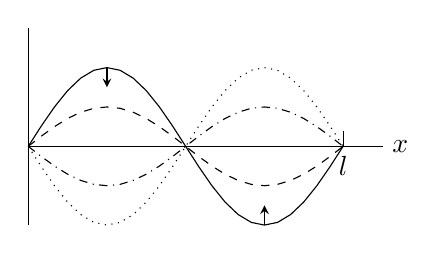
\begin{tikzpicture}
\draw(0,0)--(4.5,0)node[right]{$x$};
\draw(0,-1)--(0,1.5);
%
\draw[domain=0:360] plot ({4/360*\x},{sin(\x)});
\draw[dashed,domain=0:360] plot ({4/360*\x},{0.5*sin(\x)});
\draw[dashdotted,domain=0:360] plot ({4/360*\x},{-0.5*sin(\x)});
\draw[dotted,domain=0:360] plot ({4/360*\x},{-1*sin(\x)});
%
\draw(4,0)node[below]{$l$}--++(0,0.2);
\draw[-stealth] (1,1)--++(0,-0.25);
\draw[-stealth] (3,-1)--++(0,0.25);
\end{tikzpicture}
\caption{مختلف $t$ پر دوسرا قائمہ انداز}
\label{شکل_جزوی_مختلف_لمحات_دوسرا_قائمہ_انداز}
\end{figure}

\موٹا{تیسرا قدم۔} \quad ظاہر ہے کہ ایک عدد حل \عددی{u_n(x,t)} عموماً ابتدائی شرائط مساوات \حوالہ{مساوات_جزوی_مساوات_موج_پ} اور مساوات \حوالہ{مساوات_جزوی_مساوات_موج_ت} کو مطمئن نہیں کر سکتا ہے۔اب چونکہ مساوات \حوالہ{مساوات_جزوی_مساوات_موج_الف} خطی اور ہم جنسی ہے لہٰذا بنیادی مسئلہ \حوالہ{مسئلہ_جزوی_بنیادی} کے تحت مساوات \حوالہ{مساوات_جزوی_مساوات_موج_الف} کی محدود تعداد کے حلوں \عددی{u_n} کا مجموعہ بھی مساوات \حوالہ{مساوات_جزوی_مساوات_موج_الف} کا حل ہو گا۔  اس طرح ایسا حل جو  ابتدائی شرائط مساوات \حوالہ{مساوات_جزوی_مساوات_موج_پ} اور مساوات \حوالہ{مساوات_جزوی_مساوات_موج_ت} کو مطمئن کرتا ہو حاصل کرنے کی خاطر ہم لامتناہی تسلسل
\begin{align}\label{مساوات_جزوی_مساوات_موج_ڈ}
u(x,t)=\sum_{n=1}^{\infty} u_n(x,t)=\sum_{n=1}^{\infty} (B_n\cos \lambda_n t+B^*_n\sin \lambda_n t)\sin \frac{n\pi}{l}x
\end{align}
پر غور کرتے ہیں۔مساوات \حوالہ{مساوات_جزوی_مساوات_موج_ڈ} اور ابتدائی شرط مساوات \حوالہ{مساوات_جزوی_مساوات_موج_پ} سے درج ذیل لکھا جا سکتا ہے۔
\begin{align}\label{مساوات_جزوی_مساوات_موج_ذ}
u(x,0)=\sum_{n=1}^{\infty} B_n\sin \frac{n\pi}{l}x=f(x)
\end{align} 
یوں اگر مساوات \حوالہ{مساوات_جزوی_مساوات_موج_ڈ} نے مساوات \حوالہ{مساوات_جزوی_مساوات_موج_پ} کو مطمئن کرنا ہو تب تب عددی سر \عددی{B_n}  اس طرح منتخب کرنے ہوں گے کہ \عددی{u(x,0)} تفاعل \عددی{f(x)} کی فوریئر سائن تسلسل ہو۔یوں  مساوات \حوالہ{مساوات_فوریئر_نصف_حلقہ_توسیع_طاق_عددی_سر} سے
\begin{align}\label{مساوات_جزوی_مساوات_موج_ر}
B_n=\frac{2}{l}\int_0^l f(x)\sin \frac{n\pi x}{l}\dif x\quad \quad \quad n=1,2,\cdots
\end{align}
حاصل ہوتا ہے۔
اسی طرح مساوات \حوالہ{مساوات_جزوی_مساوات_موج_ڈ} کا \عددی{t} کے ساتھ تفرق لے کر اور ابتدائی شرط  مساوات \حوالہ{مساوات_جزوی_مساوات_موج_ت} استعمال کرتے ہوئے درج ذیل لکھا جا سکتا ہے۔ 
\begin{align*}
\left. \frac{\partial u}{\partial t}\right|_{t=0}&=\left[\sum_{n=1}^{\infty} (-B_n\lambda_n\sin \lambda_nt+B^*_n\lambda_n\cos \lambda_nt)\sin\frac{n\pi x}{l}\right]_{t=0}\\
&=\sum_{n=1}^{\infty} B^*_n\lambda_n\sin\frac{n\pi x}{l} =g(x)
\end{align*}
یوں اگر مساوات \حوالہ{مساوات_جزوی_مساوات_موج_ڈ} نے مساوات \حوالہ{مساوات_جزوی_مساوات_موج_ت} کو مطمئن کرنا ہو تب تب عددی سر \عددی{B^*_n}  اس طرح منتخب کرنے ہوں گے کہ \عددی{t=0} پر  \عددی{\tfrac{\partial u}{\partial t}} تفاعل \عددی{g(x)} کی فوریئر سائن تسلسل ہو۔ یوں مساوات \حوالہ{مساوات_فوریئر_نصف_حلقہ_توسیع_طاق_عددی_سر} سے 
\begin{align*}
B^*_n\lambda_n=\frac{2}{l}\int_0^l g(x)\sin \frac{n\pi x}{l} \dif x
\end{align*}
اور چونکہ \عددی{\lambda_n=\tfrac{cn\pi}{l}} ہے لہٰذا
\begin{align}\label{مساوات_جزوی_مساوات_موج_ڑ}
B^*_n=\frac{2}{cn\pi}\int_0^l g(x)\sin \frac{n\pi x}{l}\dif x\quad \quad \quad n=1,2,\cdots
\end{align}
لکھا جا سکتا ہے۔

مساوات \حوالہ{مساوات_جزوی_مساوات_موج_ر} اور مساوات \حوالہ{مساوات_جزوی_مساوات_موج_ڑ} میں حاصل کیے گئے عددی سر کو مساوات \حوالہ{مساوات_جزوی_مساوات_موج_ڈ} میں پر کرنے سے حاصل تسلسل \عددی{u(x,t)}، مساوات \حوالہ{مساوات_جزوی_مساوات_موج_الف} کا ایسا حل ہو گا جو مساوات \حوالہ{مساوات_جزوی_مساوات_موج_ب}، مساوات \حوالہ{مساوات_جزوی_مساوات_موج_پ} اور مساوات \حوالہ{مساوات_جزوی_مساوات_موج_ت} کی شرائط کو مطمئن کرے گا بشرطیکہ  حاصل \عددی{u(x,t)} مرتکز ہو اور اس  کی \عددی{x} اور \عددی{t} کے ساتھ جزو در جزو  دو  درجی تفرق لینے سے حاصل تسلسل مرتکز   ہو اور ان کے مجموعے  بالترتیب \عددی{\tfrac{\partial^{\,2}u}{\partial x^2}} اور \عددی{\tfrac{\partial^{\,2}u}{\partial t^2}} کے برابر ہوں جو استمراری ہیں۔

اب تک مساوات \حوالہ{مساوات_جزوی_مساوات_موج_ڈ} محض ریاضی حل کے طور پر سامنے آیا ہے۔آئیں اس کی اصل حقیقت کو قائم کریں۔ہم اپنی آسانی کی خاطر ابتدائی رفتار \عددی{g(x)} صفر لیتے ہیں۔یوں \عددی{B^*_n=0} ہوں  گے لہٰذا مساوات \حوالہ{مساوات_جزوی_مساوات_موج_ڈ} درج ذیل صورت اختیار کرے گا۔
\begin{align}\label{مساوات_جزوی_متحرک_موج_الف}
u(x,t)=\sum_{n=1}^{\infty} B_n\cos \lambda_n t\sin\frac{n\pi x}{l},\quad \lambda_n=\frac{cn\pi}{l}
\end{align}
ہم ضمیمہ \حوالہ{ضمیمہ_مفید_معلومات} کا کلیہ \حوالہ{مساوات_ضمیمہ_مفید_گیارہ} استعمال کرتے ہوئے
\begin{align*}
\cos \frac{cn\pi}{l}t\,\sin\frac{n\pi}{l}x=\frac{1}{2}\big[\sin\big\{\frac{n\pi}{l}(x-ct)\big\}+\sin\big\{\frac{n\pi}{l}(x+ct)\big\}\big]
\end{align*}
لکھ سکتے ہیں جس کو  مساوات \حوالہ{مساوات_جزوی_متحرک_موج_الف}  میں پر کرتے ہوئے درج ذیل ملتا ہے۔
\begin{align*}
u(x,t)=\frac{1}{2}\sum_{n=1}^{\infty}B_n \sin\big\{\frac{n\pi}{l}(x-ct)\big\}+\frac{1}{2}\sum_{n=1}^{\infty}B_n \sin\big\{\frac{n\pi}{l}(x+ct)\big\}
\end{align*}
آپ دیکھ سکتے ہیں کہ مساوات \حوالہ{مساوات_جزوی_مساوات_موج_ذ} میں \عددی{x} کی جگہ \عددی{x-ct} اور \عددی{x+ct} پر کرنے سے یہی دو تسلسل حاصل ہوتے ہیں لہٰذا ہم درج ذیل لکھ سکتے ہیں
\begin{align}\label{مساوات_جزوی_متحرک_موج_ب}
u(x,t)=\frac{1}{2}[f^*(x-ct)+f^*(x+ct)]
\end{align}
جہاں \عددی{f} کی طاق دوری توسیع جس کا دوری عرصہ \عددی{2l} ہو تفاعل \عددی{f^*} ہے (شکل \حوالہ{شکل_جزوی_طاق_توسیع})۔چونکہ وقفہ \عددی{0\le x\le l} پر ابتدائی انحراف \عددی{f(x)} استمراری ہے جبکہ  \عددی{x=0} اور \عددی{x=l} پر انحراف صفر ہے لہٰذا مساوات \حوالہ{مساوات_جزوی_متحرک_موج_ب} سے ظاہر ہے کہ \عددی{u(x,t)} دونوں متغیرات \عددی{x} اور \عددی{t} کی تمام قیمتوں پر استمراری ہو گا۔مساوات \حوالہ{مساوات_جزوی_متحرک_موج_ب} کا تفرق لیتے ہوئے ہم دیکھتے ہیں کہ یہ مساوات \حوالہ{مساوات_جزوی_مساوات_موج_الف} کا حل ہے بشرطیکہ  وقفہ \عددی{0<x<l} پر \عددی{f(x)} دو مرتبہ قابل تفرق ہو اور \عددی{x=0} اور \عددی{x=l} پر اس کے یک طرفہ دو درجی تفرق پائے جاتے ہوں جن کی قیمت صفر کے برابر ہو۔اس طرح یہ حقیقت قائم ہوتی ہے کہ ان شرائط پر پورا اترتا ہوا تسلسل \عددی{u(x,t)} مساوات \حوالہ{مساوات_جزوی_مساوات_موج_الف} کا ایسا حل ہو گا جو  مساوات \حوالہ{مساوات_جزوی_مساوات_موج_ب}، مساوات \حوالہ{مساوات_جزوی_مساوات_موج_پ} اور مساوات \حوالہ{مساوات_جزوی_مساوات_موج_ت} کی شرائط کو مطمئن کرتا ہے ۔
\begin{figure}
\centering
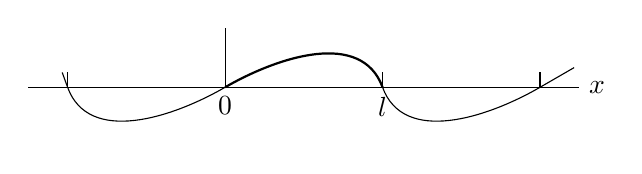
\begin{tikzpicture}
\draw(-2.5,0)--(4.5,0)node[right]{$x$};
\draw(0,0)node[below]{$0$}--(0,0.75);
\draw[thick](0,0) to [out=30,in=110] ++(2,0)node[below]{$l$};
\draw(2,0) to [out=-70,in=-150]++(2,0) --++(30:0.5);
\draw(0,0) to [out=-150,in=-70]++(-2,0)--++(110:0.2);
\draw(-2,0)--++(0,0.2);
\draw(2,0)--++(0,0.2);
\draw(4,0)--++(0,0.2);
\end{tikzpicture}
\caption{$f(x)$ کی طاق توسیع}
\label{شکل_جزوی_طاق_توسیع}
\end{figure}

اگر \عددی{f'(x)} اور \عددی{f''(x)} محض ٹکڑوں میں استمراری (حصہ \حوالہ{حصہ_لاپلاس_بدل_الٹ_بدل_خطیت}) ہوں، یا اگر وقفہ کے سروں پر یک طرفہ تفرقات غیر صفر ہوں تب ہر ایک \عددی{t} کے لئے محدود تعداد کی \عددی{x} قیمتوں پر مساوات \حوالہ{مساوات_جزوی_مساوات_موج_الف} کے \عددی{u} کی دو درجی تفرقات غیر معین ہوں گے۔ان نقطوں کے علاوہ باقی تمام نقطوں پر \عددی{u} مساوات موج کو مطمئن کرے گی لہٰذا ہم \عددی{u(x,t)} کو وسیع معنوں میں مسئلے کا حل تصور کر سکتے ہیں۔مثال کے طور پر تکونی ابتدائی انحراف کی صورت میں حاصل حل اس نوعیت کا ہو گا۔
\begin{figure}
\centering
\begin{tikzpicture}
\draw(-2,0)--(7,0)node[right]{$x$};
\draw(0,-1.7)--(0,1);
%
\draw(-2,-1) to [out=-20,in=-135]++(2,1)node[ocirc]{} to [out=45,in=180]++(1,1)node[above]{$f^*(x)$} to [out=0,in=180]++(1,-0.7) to [out=0,in=180]++(0.5,0.2) to [out=0,in=90]++(0.5,-0.5);
\draw[dashed](1.5,-1) to [out=-20,in=-135]++(2,1)to [out=45,in=180]++(1,1)node[above,solid]{$f^*(x-ct)$} to [out=0,in=180]++(1,-0.7) to [out=0,in=180]++(0.5,0.2) to [out=0,in=90]++(0.5,-0.5);
\draw(3.5,0)--++(0,-1.7);
\draw[stealth-stealth] (0,-1.7)--++(3.5,0)node[pos=0.5,fill=white]{$ct$};
\end{tikzpicture}
\caption{مساوات \حوالہ{مساوات_جزوی_متحرک_موج_ب} کی معنی}
\label{شکل_جزوی_موج_حرکت}
\end{figure}

آئیں   مساوات \حوالہ{مساوات_جزوی_متحرک_موج_ب} کی طبعی معنی سمجھتے ہیں۔جیسا شکل \حوالہ{شکل_جزوی_موج_حرکت} میں دکھایا گیا ہے، \عددی{f^*(x)} کی ترسیم کو \عددی{ct} اکائیاں دائیں منتقل کرنے سے \عددی{f^*(x-ct)} کی ترسیم حاصل ہوتی ہے۔ اس کا مطلب ہے کہ \عددی{f^*(x-ct),\,\, (c>0)} ایسی موج کو ظاہر کرتا ہے جو بڑھتے \عددی{t} کے ساتھ دائیں جانب کو حرکت کرتی ہے۔اسی طرح \عددی{f^*(x+ct),\,\, (c>0)} ایسی موج کو ظاہر کرتا ہے جو بڑھتے \عددی{t} کے ساتھ بائیں جانب کو حرکت کرتی ہے اور \عددی{u(x,t)} ان دونوں کا مجموعہ ہے۔

%======================

\begin{figure}
\centering
\begin{tikzpicture}
\pgfmathsetmacro{\kks}{-1.5}
\pgfmathsetmacro{\khs}{-5}
%
\pgfmathsetmacro{\ang}{30}
\pgfmathsetmacro{\l}{1}
\pgfmathsetmacro{\h}{\l*tan(\ang)}
%
\pgfmathsetmacro{\a}{1*\l}
\pgfmathsetmacro{\b}{2*\l-\a}
\pgfmathsetmacro{\aa}{\a/cos(\ang)}
\pgfmathsetmacro{\bb}{\b/cos(\ang)}
%
\draw(0,0)node[below]{$0$}--(2,0)node[below]{$l$};
\draw(0,0)--++(0,0.2);
\draw(2,0)--++(0,0.2);
%
\draw[thick](\a,\h)--++(-180+\ang:\aa);
\draw[thick](\a,\h)--++(-\ang:\bb)node[pos=0.5,above right]{$\tfrac{1}{2}f^*(x)$};
%=================
\begin{scope}[shift={(\khs,0)}]
\pgfmathsetmacro{\hh}{2*\h-2*(\l-\a)*tan(\ang)}
%
\draw(0,0)node[below]{$0$}--(2,0)node[below]{$l$};
\draw(0,0)--++(0,0.2);
\draw(2,0)--++(0,0.2);
%
\draw[thick] (0,0)--(\a,\hh)--(2*\l-\a,\hh)--(2*\l,0);
\draw(\a,\hh)node[left]{$u(x,0)$};
\draw(0,\hh/2)node[left]{$t=0$};
\end{scope}
%=========================
%==========================
\begin{scope}[shift={(0,1*\kks)}]
\pgfmathsetmacro{\a}{2/3*\l}
\pgfmathsetmacro{\b}{2*\l-\a}
\pgfmathsetmacro{\aa}{\a/cos(\ang)}
\pgfmathsetmacro{\bb}{\b/cos(\ang)}
%
\draw(0,0)--(2,0);
\draw(0,0)--++(0,0.2);
\draw(2,0)--++(0,0.2);
%
\draw[thick](\a,\h)--++(-180+\ang:\aa);
\draw[thick](\a,\h)--++(-\ang:\bb);
%
\draw[thick,dashed] (\b,\h)--++(-\ang:\aa);
\draw[thick,dashed](\b,\h)--++(-180+\ang:\bb);
%
\draw[-stealth] (\a,1.2*\h)--++(-0.5,0)node[left]{$\tfrac{1}{2}f^*(x+\tfrac{l}{5})$};
\draw[-stealth,dashed] (2*\l-\a,1.2*\h)--++(0.5,0)node[right]{$\tfrac{1}{2}f^*(x-\tfrac{l}{5})$};
%=================
\begin{scope}[shift={(\khs,0)}]
\pgfmathsetmacro{\hh}{2*\h-2*(\l-\a)*tan(\ang)}
%
\draw(0,0)--(2,0);
\draw(0,0)--++(0,0.2);
\draw(2,0)--++(0,0.2);
%
\draw[thick] (0,0)--(\a,\hh)--(2*\l-\a,\hh)--(2*\l,0);
\draw(0,\hh/2)node[left]{$t=\tfrac{l}{5c}$};
\end{scope}
\end{scope}
%============================
%==================================
\begin{scope}[shift={(0,2*\kks)}]
\pgfmathsetmacro{\a}{1/3*\l}
\pgfmathsetmacro{\b}{2*\l-\a}
\pgfmathsetmacro{\aa}{\a/cos(\ang)}
\pgfmathsetmacro{\bb}{\b/cos(\ang)}
%
\draw(0,0)--(2,0);
\draw(0,0)--++(0,0.2);
\draw(2,0)--++(0,0.2);
%
\draw[thick](\a,\h)--++(-180+\ang:\aa);
\draw[thick](\a,\h)--++(-\ang:\bb);
%
\draw[thick,dashed] (\b,\h)--++(-\ang:\aa);
\draw[thick,dashed](\b,\h)--++(-180+\ang:\bb);
\draw[] (0,\h/2)node[left]{$\tfrac{1}{2}f^*(x+\tfrac{2l}{5})$};
\draw[] (2*\l,\h/2)node[right]{$\tfrac{1}{2}f^*(x-\tfrac{2l}{5})$};
%=================
\begin{scope}[shift={(\khs,0)}]
\pgfmathsetmacro{\hh}{2*\h-2*(\l-\a)*tan(\ang)}
%
\draw(0,0)--(2,0);
\draw(0,0)--++(0,0.2);
\draw(2,0)--++(0,0.2);
%
\draw[thick] (0,0)--(\a,\hh)--(2*\l-\a,\hh)--(2*\l,0);
\draw(0,\hh/2)node[left]{$t=\tfrac{2l}{5c}$};
\end{scope}
\end{scope}
%======================
%=============================
\begin{scope}[shift={(0,3*\kks)}]
\pgfmathsetmacro{\a}{0*\l}
\pgfmathsetmacro{\b}{2*\l-\a}
\pgfmathsetmacro{\aa}{\a/cos(\ang)}
\pgfmathsetmacro{\bb}{\b/cos(\ang)}
%
\draw(0,0)--(2,0);
\draw(0,0)--++(0,0.2);
\draw(2,0)--++(0,0.2);
%
\draw[thick](\a,\h)--++(-180+\ang:\aa);
\draw[thick](\a,\h)--++(-\ang:\bb);
%
\draw[thick,dashed] (\b,\h)--++(-\ang:\aa);
\draw[thick,dashed](\b,\h)--++(-180+\ang:\bb);
\draw[] (0,\h/2)node[left]{$\tfrac{1}{2}f^*(x+\tfrac{l}{2})$};
\draw[] (2*\l,\h/2)node[right]{$\tfrac{1}{2}f^*(x-\tfrac{l}{2})$};
\begin{scope}[shift={(\khs,0)}]
\pgfmathsetmacro{\hh}{2*\h-2*(\l-\a)*tan(\ang)}
%
\draw(0,0)--(2,0);
\draw(0,0)--++(0,0.2);
\draw(2,0)--++(0,0.2);
%
\draw[thick] (0,0)--(\a,\hh)--(2*\l-\a,\hh)--(2*\l,0);
\draw(0,\hh/2)node[left]{$t=\tfrac{l}{2c}$};
\end{scope}
\end{scope}
%======================================
%======================================
%===================================
\begin{scope}[shift={(0,4*\kks)}]
\pgfmathsetmacro{\a}{1/3*\l}
\pgfmathsetmacro{\b}{2*\l-\a}
\pgfmathsetmacro{\aa}{\a/cos(\ang)}
\pgfmathsetmacro{\bb}{\b/cos(\ang)}
%
\draw(0,0)--(2,0);
\draw(0,0)--++(0,0.2);
\draw(2,0)--++(0,0.2);
%
\draw[thick,dashed](\a,-\h)--++(180-\ang:\aa);
\draw[thick,dashed](\a,-\h)--++(\ang:\bb);
%
\draw[thick] (\b,-\h)--++(\ang:\aa);
\draw[thick](\b,-\h)--++(180-\ang:\bb);
\draw[] (0,\h/2)node[left]{$\tfrac{1}{2}f^*(x+\tfrac{3l}{5})$};
\draw[] (2*\l,\h/2)node[right]{$\tfrac{1}{2}f^*(x-\tfrac{3l}{5})$};
\begin{scope}[shift={(\khs,0)}]
\pgfmathsetmacro{\hh}{2*\h-2*(\l-\a)*tan(\ang)}
%
\draw(0,0)--(2,0);
\draw(0,0)--++(0,0.2);
\draw(2,0)--++(0,0.2);
%
\draw[thick] (0,0)--(\a,-\hh)--(2*\l-\a,-\hh)--(2*\l,0);
\draw(0,0)node[left]{$t=\tfrac{3l}{5c}$};
\end{scope}
\end{scope}
%==================================
%====================================
\begin{scope}[shift={(0,5*\kks)}]
\pgfmathsetmacro{\a}{2/3*\l}
\pgfmathsetmacro{\b}{2*\l-\a}
\pgfmathsetmacro{\aa}{\a/cos(\ang)}
\pgfmathsetmacro{\bb}{\b/cos(\ang)}
%
\draw(0,0)--(2,0);
\draw(0,0)--++(0,0.2);
\draw(2,0)--++(0,0.2);
%
\draw[thick,dashed](\a,-\h)--++(180-\ang:\aa);
\draw[thick,dashed](\a,-\h)--++(\ang:\bb);
%
\draw[thick] (\b,-\h)--++(\ang:\aa);
\draw[thick](\b,-\h)--++(180-\ang:\bb);
\draw[] (0,\h/2)node[left]{$\tfrac{1}{2}f^*(x+\tfrac{4l}{5})$};
\draw[] (2*\l,\h/2)node[right]{$\tfrac{1}{2}f^*(x-\tfrac{4l}{5})$};
\begin{scope}[shift={(\khs,0)}]
\pgfmathsetmacro{\hh}{2*\h-2*(\l-\a)*tan(\ang)}
%
\draw(0,0)--(2,0);
\draw(0,0)--++(0,0.2);
\draw(2,0)--++(0,0.2);
%
\draw[thick] (0,0)--(\a,-\hh)--(2*\l-\a,-\hh)--(2*\l,0);
\draw(0,0)node[left]{$t=\tfrac{4l}{5c}$};
\end{scope}
\end{scope}
%==========================
%============================
\begin{scope}[shift={(0,6*\kks)}]
\pgfmathsetmacro{\a}{1*\l}
\pgfmathsetmacro{\b}{2*\l-\a}
\pgfmathsetmacro{\aa}{\a/cos(\ang)}
\pgfmathsetmacro{\bb}{\b/cos(\ang)}
%
\draw(0,0)--(2,0);
\draw(0,0)--++(0,0.2);
\draw(2,0)--++(0,0.2);
%
\draw[thick] (\b,-\h)--++(\ang:\aa);
\draw[thick](\b,-\h)--++(180-\ang:\bb);
\draw[] (\a,-\h/2)++(-1,0)node[left]{$\substack{\tfrac{1}{2}f^*(x+l)\\=\tfrac{1}{2}f^*(x-l)}$};
\begin{scope}[shift={(\khs,0)}]
\pgfmathsetmacro{\hh}{2*\h-2*(\l-\a)*tan(\ang)}
%
\draw(0,0)--(2,0);
\draw(0,0)--++(0,0.2);
\draw(2,0)--++(0,0.2);
%
\draw[thick] (0,0)--(\a,-\hh)--(2*\l-\a,-\hh)--(2*\l,0);
\draw(0,0)node[left]{$t=\tfrac{l}{c}$};
\end{scope}
\end{scope}
\end{tikzpicture}
\caption{مثال \حوالہ{مثال_جزوی_تکونی_انحراف} کا مختلف لمحات پر دائیں کو اور بائیں کو حرکت کرتے اجزاء اور ان کا مجموعہ حل $u(x,t)$}
\label{شکل_مثال_جزوی_تکونی_انحراف}
\end{figure}
%================
\ابتدا{مثال}\شناخت{مثال_جزوی_تکونی_انحراف}\quad تکونی ابتدائی انحراف کی صورت میں تار کی ارتعاش\\
مساوات موج \حوالہ{مساوات_جزوی_مساوات_موج_الف} کا حل تکونی ابتدائی انحراف
\begin{align*}
f(x)=
\begin{cases}
\frac{2k}{l}x&0<x<\frac{l}{2}\\
\frac{2k}{l}(l-x)&\frac{l}{2}<x<l
\end{cases}
\end{align*}
اور ابتدائی رفتار صفر \عددی{g(x)=0} کی صورت میں حاصل کریں۔\\
حل: چونکہ \عددی{g(x)\equiv 0} ہے لہٰذا مساوات \حوالہ{مساوات_جزوی_متحرک_موج_الف} میں \عددی{B^*_n=0} ہو گا جبکہ \عددی{B_n} کو صفحہ \حوالہصفحہ{مساوات_فوریئر_تکونی_دھڑکن_عددی_سر_ب} پر مساوات \حوالہ{مساوات_فوریئر_تکونی_دھڑکن_عددی_سر_ب} دے گی۔یوں  مساوات \حوالہ{مساوات_جزوی_متحرک_موج_الف} درج ذیل صورت اختیار کرے گی۔
\begin{align*}
u(x,t)=\frac{8k}{\pi^2}\big[\frac{1}{1^2}\sin \frac{\pi}{l}x\cos\frac{\pi c}{l}t-\frac{1}{3^2}\sin \frac{3\pi}{l}x\cos\frac{3\pi c}{l}t+-\cdots\big]
\end{align*}
اس حل کی ترسیم کھینچنے کی خاطر ہم \عددی{u(x,0)=f(x)} سے شروع کرتے ہوئے مساوات \حوالہ{مساوات_جزوی_متحرک_موج_ب} کی مدد لیتے ہیں۔یوں شکل \حوالہ{شکل_مثال_جزوی_تکونی_انحراف} حاصل ہوتی ہے۔
\انتہا{مثال}
%======================

\حصہء{سوالات}
سوال \حوالہ{سوال_جزوی_انحراف_تار_الف} تا سوال \حوالہ{سوال_جزوی_انحراف_تار_ب} میں تار کی لمبائی \عددی{l=\pi} اور \عددی{c^2=\tfrac{T}{\rho}=1} ہے۔تار کے سرے ٹھوس نقطوں کے ساتھ باندھے گئے ہیں۔ابتدائی رفتار صفر جبکہ ابتدائی انحراف \عددی{f(x)} سوال میں دی گئی ہے۔ارتعاش پذیر تار کا انحراف \عددی{u(x,t)} دریافت کریں۔

%==================
\ابتدا{سوال}\شناخت{سوال_جزوی_انحراف_تار_الف}\quad
$0.02\sin x$\\
جواب:\quad 
$u=0.02\cos t\sin x$
\انتہا{سوال}
%====================
\ابتدا{سوال}\quad
$k\sin 2x$\\
جواب:\quad
$u=k\cos 2t\sin 2x$
\انتہا{سوال}
%====================
\ابتدا{سوال}\quad
$k(\sin x-\sin 2x)$\\
جواب:\quad
$u=k(\cos t\sin x-\cos 2t\sin 2x)$
\انتہا{سوال}
%====================
\ابتدا{سوال}\شناخت{سوال_جزوی_شکل_انحراف_الف}\quad شکل \حوالہ{شکل_سوال_جزوی_شکل_انحراف_الف}-الف \\
جواب:\quad
$\tfrac{9\sqrt{3}k}{2\pi^2}(\tfrac{1}{1^2}\cos t\sin x+\tfrac{1}{2^2}\cos2t\sin 2x-\tfrac{1}{4^2}\cos 4t\sin 4x\cdots)$
%
\begin{figure}
\centering
\begin{subfigure}{0.3\textwidth}
\centering
\begin{tikzpicture}
\draw(0,0)--(2.5,0)node[right]{$x$};
\draw(0,0)--(0,1);
\draw[thick](0,0)--(2/3,0.5)--(2,0);
\draw(2/3,0)node[below]{$\tfrac{\pi}{3}$}--++(0,0.2);
\draw(2,0)node[below]{$\pi$}--++(0,0.2);
\draw[dashed](0,0.5)node[left,solid]{$0.05$}--++(2/3,0);
\end{tikzpicture}
\caption*{(الف)}
\end{subfigure}%
\begin{subfigure}{0.3\textwidth}
\centering
\begin{tikzpicture}
\draw(0,0)--(2.5,0)node[right]{$x$};
\draw(0,-1)--(0,1);
\draw[thick](0,0)--(0.5,0.5)--(1.5,-0.5)--(2,0);
\draw(0.5,0)node[below]{$\tfrac{\pi}{4}$}--++(0,0.2);
\draw(1,0)node[below]{$\tfrac{\pi}{2}$}--++(0,0.2);
\draw(1.5,0)--++(0,0.2)node[above]{$\tfrac{3\pi}{2}$};
\draw(2,0)node[below]{$\pi$}--++(0,0.2);
\draw[](0,0.5)node[left]{$\tfrac{\pi}{40}$}--++(0.2,0);
\draw[](0,-0.5)node[left]{$-\tfrac{\pi}{40}$}--++(0.2,0);
\end{tikzpicture}
\caption*{(ب)}
\end{subfigure}%
\begin{subfigure}{0.3\textwidth}
\centering
\begin{tikzpicture}
\draw(0,0)--(2.5,0)node[right]{$x$};
\draw(0,0)--(0,1);
\draw[thick](0,0)--(0.5,0.5)--(1,0)--(2,0);
\draw(0.5,0)node[below]{$\tfrac{\pi}{4}$}--++(0,0.2);
\draw(1,0)node[below]{$\tfrac{\pi}{2}$}--++(0,0.2);
\draw(2,0)node[below]{$\pi$}--++(0,0.2);
\draw[dashed](0,0.5)node[left,solid]{$k$}--(0.5,0.5);
\end{tikzpicture}
\caption*{(پ)}
\end{subfigure}%
\caption{اشکال برائے سوالات \حوالہ{سوال_جزوی_شکل_انحراف_الف}، \حوالہ{سوال_جزوی_شکل_انحراف_ب} اور \حوالہ{سوال_جزوی_شکل_انحراف_پ}}
\label{شکل_سوال_جزوی_شکل_انحراف_الف}
\end{figure}
\انتہا{سوال}
%===============
\ابتدا{سوال}\شناخت{سوال_جزوی_شکل_انحراف_ب}\quad شکل \حوالہ{شکل_سوال_جزوی_شکل_انحراف_الف}-ب \\
جواب:\quad
$\tfrac{4}{5\pi}(\tfrac{1}{2^2}\cos 2t\sin 2x-\tfrac{1}{6^2}\cos 6t\sin 6x+\tfrac{1}{10^2}\cos 10t\sin 10x\cdots)$
\انتہا{سوال}
%========================
\ابتدا{سوال}\شناخت{سوال_جزوی_شکل_انحراف_پ}\quad شکل \حوالہ{شکل_سوال_جزوی_شکل_انحراف_الف}-پ\\
جواب:\quad
$\tfrac{4k}{\pi^2}[2(\sqrt{2}-1)\cos t\sin x +\cos 2t\sin 2x-2(\sqrt{2}-\tfrac{1}{9})\cos 3t\sin 3x\cdots]$
\انتہا{سوال}
%========================
\ابتدا{سوال}\quad
$kx(x-\pi)$\\
جواب:\quad
$\tfrac{8k}{\pi}(\tfrac{1}{1^2}\cos t\sin x-\tfrac{1}{3^2}\cos 3t\sin 3x-\tfrac{1}{5^2}\cos 5t\sin 5x\cdots)$
\انتہا{سوال}
%======================
\ابتدا{سوال}\quad 
\begin{align*}
f(x)=
\begin{cases}
kx^2&0<x<\frac{\pi}{2}\\
k(x-\pi)^2&\frac{\pi}{2}<x<\pi
\end{cases}
\end{align*}
جواب:\quad
$4k[(1-\tfrac{2}{\pi})\cos t\sin x-\tfrac{1}{9}(1+\tfrac{2}{3\pi})\cos 3t\sin 3x\cdots]$
\انتہا{سوال}
%===========================
\ابتدا{سوال}\شناخت{سوال_جزوی_انحراف_تار_ب}\quad 
\begin{align*}
f(x)=
\begin{cases}
kx^2&0<x<\frac{\pi}{2}\\
-k(x-\pi)^2&\frac{\pi}{2}<x<\pi
\end{cases}
\end{align*}
جواب:\quad
$k(\tfrac{\pi}{2}-\tfrac{2}{\pi})\cos 2t\sin 2x+\tfrac{k\pi}{4}\cos 4t\sin 4x+k(\tfrac{\pi}{6}-\tfrac{2}{27\pi})\cos 6t\sin 6x\cdots$
\انتہا{سوال}
%===========================
سوال \حوالہ{سوال_جزوی_ابتدائی_رفتار_اور_انحراف_الف} تا سوال \حوالہ{سوال_جزوی_ابتدائی_رفتار_اور_انحراف_ب} میں \عددی{c^2=1} ہے، تار کی لمبائی \عددی{l=\pi} ہے اور تار کے سرے ٹھوس نقطوں سے بندھے ہیں۔ابتدائی رفتار \عددی{g(x)} اور ابتدائی انحراف \عددی{f(x)} ہیں۔ارتعاش پذیر تار کی انحراف \عددی{u(x,t)} دریافت کریں۔

%============
\ابتدا{سوال}\شناخت{سوال_جزوی_ابتدائی_رفتار_اور_انحراف_الف}\quad
$f=0,\quad g=kx \quad (0\le x\le \tfrac{\pi}{2});\quad g(x)=k(\pi-x)\quad (\tfrac{\pi}{2}\le x\le \pi)$\\
جواب:\quad
$\tfrac{4k}{\pi}(\tfrac{1}{1^3}\sin t\sin x-\tfrac{1}{3^3}\sin 3t\sin 3x+\tfrac{1}{5^3}\sin 5t\sin 5x\cdots)$
\انتہا{سوال}
%==================
\ابتدا{سوال}\quad
$f=0,\quad g=k\sin 3x$\\
جواب:\quad
$\tfrac{k}{3}\sin 3t\sin 3x$
\انتہا{سوال}
%==================
\ابتدا{سوال}\شناخت{سوال_جزوی_ابتدائی_رفتار_اور_انحراف_ب}\quad
$f=k\sin 2x,\quad g=-k\sin 2x$\\
جواب:\quad
$-\tfrac{k}{2}\sin 2t\sin 2x$
\انتہا{سوال}
%==================
\ابتدا{سوال}\quad
تناو \عددی{T} چار گنا کرنے سے بنیادی انداز کی تعدد پر کیا اثر ہو گا؟\\
جواب:\quad چونکہ \عددی{c^2=\tfrac{T}{\rho}} ہے لہٰذا \عددی{T} چار گنا کرنے سے \عددی{c} دگنا ہو گا جس سے بنیادی انداز کی تعدد دگنی ہو گی۔
\انتہا{سوال}
%=====================
\ابتدا{سوال}\quad
تار کی لمبائی  چار گنا کرنے سے بنیادی انداز کی تعدد پر کیا اثر ہو گا؟\\
جواب:\quad بنیادی انداز کی تعدد چار گنا کم ہو گی۔
\انتہا{سوال}
%=====================
سوال \حوالہ{سوال_جزوی_علیحدگی_متغیرات_الف} تا سوال \حوالہ{سوال_جزوی_علیحدگی_متغیرات_ب} میں دیے گئے جزوی تفرقی مساوات کو علیحدگی متغیرات کے طریقہ سے حل کریں۔

%=================
\ابتدا{سوال}\شناخت{سوال_جزوی_علیحدگی_متغیرات_الف}\quad
$u_x+u_y=0$\\
جواب:\quad
$u=ce^{k(x+y)}$
\انتہا{سوال}
%========================
\ابتدا{سوال}\quad
$u_x-u_y=0$\\
جواب:\quad
$u=ce^{k(x-y)}$
\انتہا{سوال}
%========================
\ابتدا{سوال}\quad
$xu_x-yu_y=0$\\
جواب:\quad
$u=kxy$
\انتہا{سوال}
%========================
\ابتدا{سوال}\quad
$u_x-yu_y=0$\\
جواب:\quad
$u=cy^ke^{kx}$
\انتہا{سوال}
%========================
\ابتدا{سوال}\quad
$yu_x-xu_y=0$\\
جواب:\quad
$u=ce^{k(x^2+y^2)}$
\انتہا{سوال}
%========================
\ابتدا{سوال}\quad
$u_x+u_y=2(x+y)u$\\
جواب:\quad
$u=ce^{x^2+y^2+k(x-y)}$
\انتہا{سوال}
%========================
\ابتدا{سوال}\quad
$u_{xx}+u_{yy}=0$\\
جواب:\quad
$u=(A\cos kx+B\sin kx)(Ce^{ky}+De^{-ky})$
\انتہا{سوال}
%========================
\ابتدا{سوال}\شناخت{سوال_جزوی_علیحدگی_متغیرات_ب}\quad
$u_{xy}-u=0$\\
جواب:\quad
$u=ce^{x+y}$
\انتہا{سوال}
%========================
سوال \حوالہ{سوال_جزوی_تار_جبری_الف} تا سوال \حوالہ{سوال_جزوی_تار_جبری_ٹ} \موٹا{لچکدار تار کی جبری ارتعاش} پر مبنی ہیں۔

%====================
\ابتدا{سوال}\شناخت{سوال_جزوی_تار_جبری_الف}\quad لچک دار تار کی جبری ارتعاش کا الجبرائی نمونہ درج ذیل جزوی تفرقی مساوات  ہے جہاں اکائی لمبائی پر  بیرونی قوت \عددی{P(x,t)}  تار کے عمودی عمل کرتا ہے۔
\begin{align}\label{مساوات_جزوی_تار_جبری_الف}
u_{tt}=c^2u_{xx}+\frac{P}{\rho}
\end{align} 
دیے گئے مسئلے سے اس جزوی تفرقی مساوات کو حاصل کریں۔
\انتہا{سوال}
%====================
\ابتدا{سوال}\شناخت{سوال_جزوی_تار_جبری_ب}\quad
سائن نما بیرونی قوت \عددی{P=A\rho \sin \omega t} کی صورت میں درج ذیل ثابت کریں
\begin{align*}
\frac{P}{\rho}=A\sin \omega t=\sum_{n=1}^{\infty} k_n(t)\sin \frac{n\pi x}{l}
\end{align*}
جہاں 
$k_n(t)=\tfrac{2A}{n\pi}(1-\cos n\pi)\sin \omega t$
 ہے۔یوں جفت \عددی{n} کی صورت میں \عددی{k_n=0} اور طاق \عددی{n} کی صورت میں 
$k_n=\tfrac{4A}{n\pi}\sin \omega t$
ہو گا۔مزید ثابت کریں کہ مساوات \حوالہ{مساوات_جزوی_مساوات_موج_الف} میں
\begin{align*}
u(x,t)=\sum_{n=1}^{\infty} G(t)\sin \frac{n\pi x}{l}
\end{align*}
پر کرنے سے درج ذیل ملتا ہے۔
\begin{align*}
\ddot{G}_n+\lambda^2_n G_n=0,\quad \lambda_n=\frac{cn\pi}{l}
\end{align*}
\انتہا{سوال}
%===================
\ابتدا{سوال}\شناخت{سوال_جزوی_تار_جبری_پ}\quad
ثابت کریں کہ  سوال \حوالہ{سوال_جزوی_تار_جبری_ب} کے \عددی{\tfrac{P}{\rho}} اور \عددی{u} کو مساوات \حوالہ{مساوات_جزوی_تار_جبری_الف} میں پر کرنے سے درج ذیل حاصل ہوتا ہے۔
\begin{align*}
\ddot{G}_n+\lambda^2_nG_n=\frac{2A}{n\pi}(1-\cos n\pi)\sin\omega t,\quad \quad \lambda_n=\frac{cn\pi}{l}
\end{align*}  
ثابت کریں کہ \عددی{\lambda^2_n\ne \omega^2} کی صورت میں اس کا حل درج ذیل ہو گا۔
\begin{align*}
G_n(t)=B_n\cos\lambda_nt+B^*_n\sin\lambda_nt+\frac{2A(1-\cos n\pi)}{n\pi(\lambda^2_n-\omega^2)}\sin \omega t
\end{align*}
\انتہا{سوال}
%========================
\ابتدا{سوال}\شناخت{سوال_جزوی_تار_جبری_ت}\quad
ایسے \عددی{B_n} اور \عددی{B^*_n} دریافت کریں کہ \عددی{u} ابتدائی شرائط \عددی{u(x,0)=f(x)} اور \عددی{u_t(x,0)=0} کو مطمئن کرے (سوال \حوالہ{سوال_جزوی_تار_جبری_پ})۔
\انتہا{سوال}
%=====================
\ابتدا{سوال}\شناخت{سوال_جزوی_تار_جبری_ٹ}\quad
ثابت کریں کہ گمک \عددی{\lambda_n=\omega} کی صورت میں درج ذیل ہو گا۔
\begin{align*}
G_n(t)=B_n\cos \omega t+B^*_n\sin\omega t-\frac{A}{n\pi \omega}(1-\cos n\pi)t\cos \omega t
\end{align*}
\انتہا{سوال}
%=========================

\حصہ{مساوات موج کا دا لومبیغ حل}\شناخت{حصہ_جزوی_دا_لومبیغ_حل}
گزشتہ حصہ میں مساوات موج
\begin{align}\label{مساوات_جزوی_موج_مساوات_الف}
\frac{\partial^{\,2}u}{\partial t^2}=c^2\frac{\partial^{\,2}u}{\partial x^2}
\end{align}
کا حل مساوات \حوالہ{مساوات_جزوی_متحرک_موج_ب} حاصل کیا گیا۔یہی حل نہایت آسانی سے مساوات \حوالہ{مساوات_جزوی_موج_مساوات_الف} کا موزوں بدل لیتے ہوئے حاصل کیا جا سکتا ہے۔یوں نئے غیر تابع متغیرات\حاشیہد{یہاں بتلاتا چلوں کہ جزوی تفرقی مساوات کا عمومی نظریہ اس طرح کے تبادل حاصل کرنے کی قدم با قدم ترکیب پیش کرتی ہے۔}
\begin{align}\label{مساوات_جزوی_موج_مساوات_ب}
v=x+ct,\quad z=x-ct
\end{align}
متعارف کرتے ہوئے \عددی{u} کو متغیرات \عددی{v} اور \عددی{z} کا تفاعل لکھتے ہیں۔اس طرح مساوات \حوالہ{مساوات_جزوی_موج_مساوات_الف} میں تفرقات اب \عددی{v} اور \عددی{z} کے لحاظ سے زنجیری ترکیب (حصہ \حوالہ{حصہ_الاحصاء_زنجیری_ترکیب})  کی مدد سے لکھے جائیں گے۔جزوی تفرق کو زیر نوشت سے ظاہر کرتے ہوئے  مساوات \حوالہ{مساوات_جزوی_موج_مساوات_ب} سے \عددی{v_x=1} اور \عددی{z_x=1} لکھے جائیں گے۔ہم اپنی آسانی کے لئے ہم \عددی{v} اور \عددی{z} متغیرات کے تفاعل کو بھی \عددی{u} سے ظاہر کرتے ہیں۔اس طرح درج ذیل لکھا جا سکتا ہے۔
\begin{align*}
u_x=u_vv_x+u_zz_x=u_v+u_z
\end{align*}
دائیں ہاتھ پر زنجیری ترکیب لاگو کرتے ہوئے اور \عددی{v_x=1} اور \عددی{z_x=1} پر کرتے ہوئے
\begin{align*}
u_{xx}=(u_v+u_z)_x=(u_v+u_z)_vv_x+(u_v+u_z)_zz_x=u_{vv}+2u_{vz}+u_{zz}
\end{align*}
ملتا ہے۔مساوات \حوالہ{مساوات_جزوی_موج_مساوات_الف} کی دوسری تفرق کو بھی اسی طرح لکھتے ہیں۔
\begin{align*}
u_{tt}=c^2(u_{vv}-2u_{vz}+u_{zz})
\end{align*}
ان نتائج کو مساوات \حوالہ{مساوات_جزوی_موج_مساوات_الف} میں پر کرنے سے درج ذیل ملتا ہے۔
\begin{align}\label{مساوات_جزوی_موج_مساوات_پ}
u_{vz}\equiv \frac{\partial^{\,2}u}{\partial v\partial z}=0
\end{align}
آپ نے دیکھا کہ نئے متغیرات متعارف کرنے سے حاصل مساوات \حوالہ{مساوات_جزوی_موج_مساوات_پ} نہایت آسانی سے دو مرتبہ تکمل لینے سے حل ہو سکتی ہے۔ایک مرتبہ \عددی{z} کے ساتھ تکمل لینے سے
\begin{align*}
\frac{\partial u}{\partial v}=h(v)
\end{align*}
حاصل ہو گا جہاں نا معلوم تفاعل \عددی{h(v)} متغیرہ \عددی{v} کے تابع ہو سکتا ہے۔ اس کا تکمل \عددی{v} کے ساتھ لیتے ہیں
\begin{align*}
u=\int h(v)\,\dif v+\psi(z)
\end{align*}
جہاں \عددی{\psi(z)} متغیرہ \عددی{z} کا نا معلوم تفاعل ہے۔درج بالا میں تکمل کا حاصل از خود \عددی{v} کا تفاعل ہو گا جس کو نا معلوم تفاعل  \عددی{\phi(v)} لکھتے ہوئے مساوات \حوالہ{مساوات_جزوی_موج_مساوات_پ} کی مدد سے 
\begin{align}\label{مساوات_جزوی_موج_مساوات_ت}
u(x,t)=\phi(x+ct)+\psi(x-ct)
\end{align}
حاصل ہوتا ہے۔اس کو موج کی مساوات \حوالہ{مساوات_جزوی_موج_مساوات_الف} کا \اصطلاح{دا لومبیغ حل}\فرہنگ{دا لومبیغ حل}\حاشیہب{d'Alembert solution}\فرہنگ{d'Alembert solution} کہتے\حاشیہد{فرانسیسی ریاضی دان ژاں باٹِیسٹ لی غوں دا لومبیغ [1717-1783]} ہیں۔

تفاعل \عددی{\phi} اور \عددی{\psi} کو ابتدائی معلومات سے دریافت کیا جا سکتا ہے۔آئیں صفر ابتدائی رفتار اور ابتدائی انحراف \عددی{u(x,0)=f(x)} کے لئے ان تفاعل کو حاصل کریں۔

مساوات \حوالہ{مساوات_جزوی_موج_مساوات_ت} کا تفرق لیتے ہیں
\begin{align}\label{مساوات_جزوی_موج_مساوات_ٹ}
\frac{\partial u}{\partial t}=c\phi'(x+ct)-c\psi'(x-ct)
\end{align}
جہاں \عددی{(')} سے مراد قوسین میں بند پوری دلیل \عددی{x+ct} اور \عددی{x-ct} کے لحاظ سے بالترتیب  تفرق ہے۔مساوات \حوالہ{مساوات_جزوی_موج_مساوات_ت}، مساوات \حوالہ{مساوات_جزوی_موج_مساوات_ٹ} اور ابتدائی معلومات سے درج ذیل لکھا جا سکتا ہے۔
\begin{align*}
u(x,0)&=\phi(x)+\psi(x)=f(x)\\
u_t(x,0)&=c\phi'(x)-c\psi'(x)=0
\end{align*} 
آخری مساوات یعنی \عددی{\phi'=\psi'} سے \عددی{\psi=\phi+k} حاصل ہوتا ہے  جس کو پہلی مساوات کے ساتھ ملا کر \عددی{2\phi+k=f} یا \عددی{\phi=\tfrac{f-k}{2}} حاصل ہوتا ہے۔ ان حاصل کردہ \عددی{\phi} اور \عددی{\psi}  کو استعمال کرتے ہوئے مساوات \حوالہ{مساوات_جزوی_موج_مساوات_ت} کو درج ذیل لکھا جا سکتا ہے
\begin{align}\label{مساوات_جزوی_موج_مساوات_ث}
u(x,t)=\frac{1}{2}[f(x+ct)+f(x-ct)]
\end{align}
جو عین مساوات \حوالہ{مساوات_جزوی_متحرک_موج_ب} ہے۔آپ یہاں تصدیق کر سکتے ہیں کہ مساوات \حوالہ{مساوات_جزوی_متحرک_موج_ب} پر لاگو  ابتدائی سرحدی شرائط مساوات \حوالہ{مساوات_جزوی_مساوات_موج_ب} کی بنا \عددی{f} طاق ہو گا اور اس کا دوری عرصہ \عددی{2l} ہو گا۔

ہمارے اس نتیجہ کے تحت دو عدد ابتدائی شرائط اور سرحدی شرائط مل کر مساوات موج کا حل یکتا طور پر تعین کرتی ہیں۔ 

%=======================
\حصہء{سوالات}

%==============
\ابتدا{سوال}\quad
مساوات \حوالہ{مساوات_جزوی_موج_مساوات_ب} دیکھ کر \عددی{x} اور \عددی{t} کو  \عددی{v} اور \عددی{z} کی صورت  میں لکھتے ہوئے مساوات \حوالہ{مساوات_جزوی_موج_مساوات_پ} سے  مساوات \حوالہ{مساوات_جزوی_موج_مساوات_الف} حاصل کریں۔ 
\انتہا{سوال}
%=======================
سوال \حوالہ{سوال_جزوی_حرکت_موج_الف} تا سوال \حوالہ{سوال_جزوی_حرکت_موج_ب} میں مساوات \حوالہ{مساوات_جزوی_موج_مساوات_ث} استعمال کرتے ہوئے شکل  \حوالہ{شکل_مثال_جزوی_تکونی_انحراف} کی طرح مختلف لمحات پر تار کی انحراف  \عددی{u(x,t)} کی  ترسیم کھینچیں۔تار کی لمبائی اکائی \عددی{(1)} ہے اور اس کے دونوں سرے ہل نہیں سکتے  ہیں۔ابتدائی رفتار صفر ہے جبکہ ابتدائی انحراف \عددی{f(x)} ہے۔\عددی{k} کی کوئی بھی چھوٹی قیمت مثلاً \عددی{k=0.01} لیں۔

%=====================
\ابتدا{سوال}\شناخت{سوال_جزوی_حرکت_موج_الف}\quad
$f(x)=k\sin 2\pi x$
\انتہا{سوال}
%==================
\ابتدا{سوال}\quad
$f(x)=kx(1-x)$
\انتہا{سوال}
%==================
\ابتدا{سوال}\quad
$f(x)=k(x-x^3)$
\انتہا{سوال}
%==================
\ابتدا{سوال}\quad
$f(x)=k(x^2-x^4)$
\انتہا{سوال}
%==================
\ابتدا{سوال}\quad
$f(x)=k(x^3-x^5)$
\انتہا{سوال}
%==================
\ابتدا{سوال}\شناخت{سوال_جزوی_حرکت_موج_ب}\quad
$f(x)=k\sin^2 \pi x$
\انتہا{سوال}
%==================
سوال \حوالہ{سوال_جزوی_تبادل_حل_الف} تا سوال \حوالہ{سوال_جزوی_تبادل_حل_ب} میں دیے گئے تبادل استعمال کرتے ہوئے جزوی تفرقی مساوات حل کریں۔ 

%================
\ابتدا{سوال}\شناخت{سوال_جزوی_تبادل_حل_الف}\quad
$xu_{xy}=yu_{yy}+u_y\quad (v=x,\, z=xy)$
\انتہا{سوال}
%=====================
\ابتدا{سوال}\quad
$u_{xy}-u_{yy}=0\quad (v=x,\, z=x+y)$\\
جواب:\quad
$u=f_1(x)+f_2(x+y)$
\انتہا{سوال}
%=====================
\ابتدا{سوال}\شناخت{سوال_جزوی_درکار_بعد_الف}\quad
$u_{xx}+2u_{xy}+u_{yy}=0\quad (v=x,\, z=x-y)$
\انتہا{سوال}
%=====================
\ابتدا{سوال}\quad
$u_{xx}-2u_{xy}+u_{yy}=0\quad (v=x,\, z=x+y)$\\
جواب:\quad
$u=xf_1(x+y)+f_2(x+y)$
\انتہا{سوال}
%=====================
\ابتدا{سوال}\شناخت{سوال_جزوی_تبادل_حل_ب}\quad
$u_{xx}+u_{xy}-2u_{yy}=0\quad (v=x+y,\, z=2x-y)$
\انتہا{سوال}
%=====================
\ابتدا{سوال}\شناخت{سوال_جزوی_تفرقی_اقسام}\quad \موٹا{خطی جزوی تفرقی مساوات کی اقسام}\\
درج ذیل طرز کی مساوات
\begin{align}\label{مساوات_جزوی_عمومی_صورت_الف}
Au_{xx}+2Bu_{xy}+Cu_{yy}=F(x,y,u,u_x,u_y)
\end{align}
کو \عددی{AC-B^2>0} کی صورت میں \اصطلاح{بیضوی}\فرہنگ{بیضوی!جزوی تفرقی مساوات}\فرہنگ{جزوی!تفرقی بیضوی}\حاشیہب{elliptic}
\فرہنگ{elliptic!partial differential}، \عددی{AC-B^2=0} کی صورت میں \اصطلاح{قطع مکافی}\فرہنگ{قطع مکافی!جزوی تفرقی مساوات}\فرہنگ{جزوی!تفرقی قطع مکافی}\حاشیہب{parabolic}\فرہنگ{parabolic!partial differential} اور \عددی{AC-B^2<0} کی صورت میں \اصطلاح{قطع زائد}\فرہنگ{قطع زائد!جزوی تفرقی مساوات}\فرہنگ{جزوی!تفرقی قطع زائد}\حاشیہب{hyperbolic}\فرہنگ{hyperbolic!partial differential} کہتے ہیں۔یہاں \عددی{A}، \عددی{B} اور \عددی{C} از خود \عددی{x} اور \عددی{y} کے تفاعل ہو سکتے ہیں۔مساوات \حوالہ{مساوات_جزوی_عمومی_صورت_الف} سطح \عددی{xy} کی مختلف حصوں میں مختلف قسم کا ہو سکتا ہے۔تصدیق کریں کہ
\begin{align*}
\text{\RL{بیضوی ہے}}\quad u_{xx}+u_{yy}&=0\quad \text{\RL{لاپلاسی مساوات}}\\
\text{\RL{قطع مکافی ہے}}\quad u_{t}&=c^2u_{xx}\quad \text{\RL{حراری مساوات}}\\
\text{\RL{قطع زائد ہے۔}}\quad u_{tt}&=c^2u_{xx}\quad \text{\RL{جبکہ مساوات موج}}
\end{align*}
اس کے برعکس 
$yu_{xx}+u_{yy}=0$
بالائی نصف سطح پر بیضوی، \عددی{x} محور پر قطع مکافی اور نچلی نصف سطح پر قطع زائد ہے۔
\انتہا{سوال}
%====================
\ابتدا{سوال}\شناخت{سوال_جزوی_تبدیل_قطع_زائد}\quad
اگر مساوات \حوالہ{مساوات_جزوی_عمومی_صورت_الف} کی قسم قطع زائد ہو تب  \عددی{v=\phi(x,y)} اور \عددی{z=\psi(x,y)} استعمال کرتے ہوئے اس کو
$u_{vz}=R^*(v,z,u,u_v,u_z)$
صورت میں تبدیل کیا جا سکتا ہے جہاں \عددی{\phi=c_1} اور \عددی{\psi=c_2} ($c_1$ اور $c_2$ مستقل ہیں) مساوات \عددی{Ay'^2-2By'+C=0} کے حل \عددی{y=y(x)} ہیں۔تصدیق کریں کہ مساوات  \حوالہ{مساوات_جزوی_موج_مساوات_الف} کی صورت میں درج ذیل تبادل حاصل ہوں گے۔
\begin{align*}
\phi=x+ct,\quad \psi=x-ct
\end{align*}
جواب:\quad مساوات موج کو \عددی{u_{tt}-c^2u_{xx}=0} لکھ کر \عددی{A=1}، \عددی{B=0} اور \عددی{C=-c^2} ملتے ہیں۔چونکہ ہمارے متغیرات \عددی{t} اور \عددی{x} ہیں لہٰذا  مساوات \حوالہ{مساوات_جزوی_عمومی_صورت_الف} کو \عددی{1u_{tt}+0-c^2u_{xx}=0} لکھ سکتے ہیں۔یوں ہمیں \عددی{A(\tfrac{\dif x}{\dif t})^2-2B(\tfrac{\dif x}{\dif t})^2-c^2=0} یعنی \عددی{(\tfrac{\dif x}{\dif t})^2-c^2=0} یا \عددی{\tfrac{\dif x}{\dif t}=\mp c} کے حل درکار ہیں جو \عددی{x=\mp ct+k} یعنی \عددی{x\mp ct=k} ہیں۔یوں \عددی{\phi=x+ct} اور \عددی{\psi=x-ct} ملتے ہیں۔
\انتہا{سوال}
%===================
\ابتدا{سوال}\quad
اگر مساوات \حوالہ{مساوات_جزوی_عمومی_صورت_الف} کی قسم قطع مکافی ہو تب  \عددی{v=x} اور \عددی{z=\psi(x,y)} استعمال کرتے ہوئے اس کو
$u_{vv}=R^*(v,z,u,u_v,u_z)$
صورت میں تبدیل کیا جا سکتا ہے جہاں \عددی{\psi} حاصل کرنے کی ترکیب سوال \حوالہ{سوال_جزوی_تبدیل_قطع_زائد} میں دی گئی ہے۔اس حقیقت کو سوال \حوالہ{سوال_جزوی_درکار_بعد_الف} کی تفرقی مساوات کے لئے ثابت کریں۔\\
جواب:\quad
$y'^2-2y'+1=(y'-1)^2=0$
سے \عددی{y=x+c} یا \عددی{\psi(x,y)=x-y} ملتا ہے۔ \عددی{v=x} اور \عددی{z=x-y} ہیں۔ 
\انتہا{سوال}
%======================
سوال \حوالہ{سوال_جزوی_شہتیر_الف} تا سوال \حوالہ{سوال_جزوی_شہتیر_ٹ} \موٹا{شہتیر کی لرزش} میں مبنی ہیں۔

%========================
\ابتدا{سوال}\شناخت{سوال_جزوی_شہتیر_الف}\quad 
افقی شہتیر (شکل \حوالہ{شکل_جزوی_شہتیر}-الف) کی انتصابی  لرزش درج ذیل جزوی تفرقی مساوات دیتی ہے
\begin{align}\label{مساوات_جزوی_شہتیر_الف}
\frac{\partial^{\,2}u}{\partial t^2}+c^2\frac{\partial^{\,4}u}{\partial x^4}=0\quad \quad \quad c^2=\frac{EI}{\rho A}
\end{align}
جہاں \عددی{E} ینگ مقیاس لچک، محور \عددی{y} کے لحاظ سے \عددی{I}  جمودی معیار اثر، \عددی{\rho} کثافت اور \عددی{A} رقبہ عمودی تراش ہیں۔ مساوات \حوالہ{مساوات_جزوی_شہتیر_الف} میں \عددی{u=F(x)G(t)} پر کرتے ہوئے علیحدگی متغیرات سے درج ذیل حاصل کریں۔
\begin{align*}
\frac{F^{(4)}}{F}&=-\frac{\ddot{G}}{c^2G}=\beta^4=\text{مستقل},\\
F(x)&=A\cos \beta x+B\sin \beta x+C\cosh \beta x+D\sinh \beta x,\\
G(t)&=a\cos c\beta^2t+b\sin c\beta^2 t
\end{align*} 
%
\begin{figure}
\centering
\begin{subfigure}{1\textwidth}
\centering
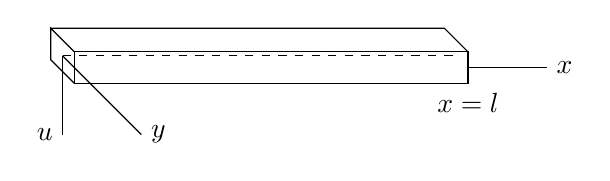
\begin{tikzpicture}[x={(1cm,0)},y={(0.5cm,-0.5cm)},z={(0,1cm)}]
\pgfmathsetmacro{\ax}{5}
\pgfmathsetmacro{\by}{0.6}
\pgfmathsetmacro{\cz}{0.4}
%
\draw(0,0,0)--++(0,0,\cz);
\draw(0,0,0)--++(0,-\by,0)--++(0,0,\cz)--++(0,\by);
\draw(0,0,0)--++(\ax,0,0)--++(0,0,\cz)coordinate(kR)--++(-\ax,0,0);
\draw(kR)--++(0,-\by,0)--++(-\ax,0,0);
%
\draw(\ax,0,1/2*\cz)--++(1,0,0)node[right]{$x$};
\draw(0,-\by/2,\cz/2)--++(0,2,0)node[right]{$y$};
\draw(0,-\by/2,\cz/2)--++(0,0,-1)node[left]{$u$};
\draw[dashed](0,-\by/2,\cz/2)--++(\ax,0,0);
\draw(\ax,0,0)node[below]{$x=l$};
\end{tikzpicture}
\caption*{(الف) شہتیر کی ساخت}
\end{subfigure}
%
\begin{subfigure}{1\textwidth}
\centering
\begin{tikzpicture}
\draw(0,0) to [out=-10,in=-170] (5,0)--++(0,0.4) to [out=-170,in=-10] (0,0.4)--(0,0);
\draw[dashed](0,0.2)node[solid,ocirc]{}--++(5,0);
\draw(5,0.2)--++(1,0)node[right]{$x$};
\draw(0,0)--++(0.3,-0.3)--++(-0.6,0)coordinate(kkL)--++(0.3,0.3);
\draw(5,0)--++(0.3,-0.3)coordinate(kR)--++(-0.6,0)coordinate(kL)--++(0.3,0.3);
\draw(kL)++(2pt,-2pt) node[ocirc]{};
\draw(kR)++(-2pt,-2pt) node[ocirc]{};
\draw[fill=gray!50!white](kkL)--++(-0.25,0)--++(0,-0.2)--++(1.1,0)--++(0,0.2)--++(-1.1,0);
\draw[fill=gray!50!white](kL)++(0,-4pt)--++(-0.25,0)--++(0,-0.2)--++(1.1,0)--++(0,0.2)--++(-1.1,0);
\draw[-latex](0,-0.6)--++(0,-0.75)node[left]{$u$};
\draw(5,-0.6)node[below]{$x=l$};
\end{tikzpicture}
\caption*{(ب) شہتیر کے سر آزاد پڑے ہیں}
\end{subfigure}
%
\begin{subfigure}{1\textwidth}
\centering
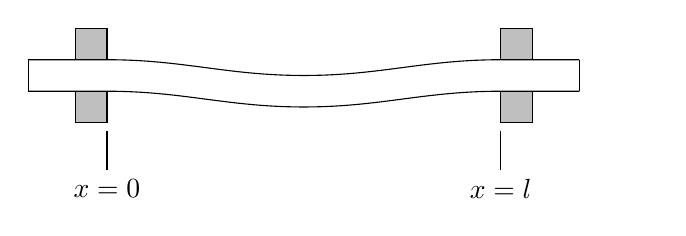
\begin{tikzpicture}
\draw(0,0)--++(1,0) to [out=0,in=180] ++(2.5,-0.2) to [out=0,in=180]++(2.5,0.2) --++(1,0);
\draw(0,0.4)--++(1,0) to [out=0,in=180] ++(2.5,-0.2) to [out=0,in=180]++(2.5,0.2) --++(1,0);
\draw(0,0)--++(0,0.4);
\draw(7,0)--++(0,0.4);
%
\draw[fill=gray!50!white](1,0)--++(0,-0.4)--++(-0.4,0)--++(0,0.4)--++(0.4,0);
\draw[fill=gray!50!white](1,0.4+0.4)--++(0,-0.4)--++(-0.4,0)--++(0,0.4)--++(0.4,0);
%
\draw[fill=gray!50!white](6.4,0)--++(0,-0.4)--++(-0.4,0)--++(0,0.4)--++(0.4,0);
\draw[fill=gray!50!white](6.4,0.4+0.4)--++(0,-0.4)--++(-0.4,0)--++(0,0.4)--++(0.4,0);
%
\draw(1,-0.5)--++(0,-0.5) node[below]{$x=0$};
\draw(6,-0.5)--++(0,-0.5)node[below]{$x=l$};
\path(7,0)--++(1,0);
\end{tikzpicture}
\caption*{(پ) شہتیر کے سر جکڑے ہیں}
\end{subfigure}
\caption{شہتیر کی لرزش}
\label{شکل_جزوی_شہتیر}
\end{figure}
\انتہا{سوال}
%=========================
\ابتدا{سوال}\شناخت{سوال_جزوی_شہتیر_ب}\quad
ابتدائی رفتار صفر لیتے ہوئے  مساوات \حوالہ{مساوات_جزوی_شہتیر_الف} کے وہ حل \عددی{u_n=F_n(x)G_n(t)} دریافت کریں جو درج ذیل ابتدائی شرائط کو مطمئن کرتے ہوں (شکل \حوالہ{شکل_جزوی_شہتیر}-ب)۔
\begin{align*}
u(0,t)&=0,\quad u(l,t)=0 \quad \text{\RL{شہتیر کے دونوں سر دیوار پر آزاد رکھے گئے ہیں}}\\
u_{xx}(0,t)&=0,\quad u_{xx}(l,t)=0\quad \text{\RL{یوں سروں پر صفر معیار اثر لہٰذا صفر گولائی ہو گی}}
\end{align*} 
جواب:\quad
\begin{align*}
F_n=\sin \frac{n\pi x}{l}, \quad G_n=a_n\cos \frac{cn^2\pi^2 t}{l^2}
\end{align*}
\انتہا{سوال}
%===========================
\ابتدا{سوال}\شناخت{سوال_جزوی_شہتیر_پ}\quad
مساوات \حوالہ{مساوات_جزوی_شہتیر_الف} کا وہ حل جو سوال \حوالہ{سوال_جزوی_شہتیر_ب} کے شرائط کے ساتھ ساتھ ابتدائی انحراف \عددی{u(x,0)=f(x)=x(l-x)} کو مطمئن کرتا ہو حاصل کریں۔
\انتہا{سوال}
%==========================
\ابتدا{سوال}\شناخت{سوال_جزوی_شہتیر_ت}\quad
شہتیر کے دونوں سروں سے جکڑنے سے کیا ابتدائی شرائط پیدا ہوں گے (شکل \حوالہ{شکل_جزوی_شہتیر}-پ)؟\\
جواب:\quad
$u(0,t)=0,\quad u(l,0)=0,\quad u_x(0,t)=0,\quad u_x(l,t)=0$
\انتہا{سوال}
%===========================
\ابتدا{سوال}\شناخت{سوال_جزوی_شہتیر_ٹ}\quad
تصدیق کریں کہ سوال \حوالہ{سوال_جزوی_شہتیر_الف} میں حاصل \عددی{F(x)} سوال \حوالہ{سوال_جزوی_شہتیر_ت} میں دی گئی شرائط کو اس صورت مطمئن کرتا ہے جب \عددی{\beta l} درج ذیل مساوات کے جذر ہوں۔
\begin{align}\label{مساوات_جزوی_شہتیر_ب}
\cosh \beta l\cos \beta l=1
\end{align}
مساوات \حوالہ{مساوات_جزوی_شہتیر_ب} کے چند حل کا تخمینہ لگائیں ۔
\انتہا{سوال}
%===========================

\حصہ{یک بعدی بہاو حرارت}
ہم جنسی مادّہ میں حرارت کی بہاو حراری مساوات (حصہ \حوالہ{حصہ_خطی_تکمل_مسئلہ_پھیلاو_نتائج})
\begin{align*}
\frac{\partial u}{\partial t}=c^2\nabla^{\,2}u\quad \quad \quad c^2=\frac{K}{\sigma \rho}
\end{align*}
دیتی ہے جہاں \عددی{u(x,y,z,t)} جسم کا درجہ حرارت، \عددی{K} جسم کی  حراری موصلیت، \عددی{\sigma} جسم کی مخصوص حراری استعداد اور \عددی{\rho} جسم کے مادّہ کی کثافت ہے۔ \عددی{\nabla^{\,2}u} درجہ حرارت \عددی{u} کا لاپلاسی ہے جو کارتیسی نظام کی محدد \عددی{x}، \عددی{y}، \عددی{z} کے لحاظ سے درج ذیل لکھا جاتا ہے۔
\begin{align*}
\nabla^{\,2}u=\frac{\partial^{\,2}u}{\partial x^2}+\frac{\partial^{\,2}u}{\partial y^2}+\frac{\partial^{\,2} u}{\partial z^2}
\end{align*}
آئیں ایک لمبی سلاخ یا تار جو \عددی{x} محور پر رکھی گئی ہو میں درجہ حرارت پر غور کرتے ہیں (شکل \حوالہ{شکل_جزوی_لمبی_سلاخ})۔یہ سلاخ ہم جنسی مادّہ سے بنی ہے اور اس کا رقبہ عمودی تراش  یکساں ہے۔اس سلاخ کے اطراف کو مکمل طور پر غیر موصل سے گھیر کر حاجز شدہ کیا گیا ہے لہٰذا سلاخ میں حرارت کی بہاو صرف لمبائی کے رخ ممکن ہے۔اس طرح \عددی{u} صرف \عددی{x} اور \عددی{t} پر منحصر ہو گا لہٰذا حراری مساوات درج ذیل \اصطلاح{یک بعدی حراری مساوات}\فرہنگ{حراری!یک بعدی مساوات}\حاشیہب{one dimensional heat equation}\فرہنگ{heat!one dimensional equation} کی صورت اختیار کرے گی۔
\begin{figure}
\centering
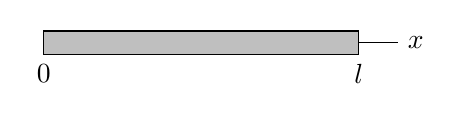
\begin{tikzpicture}
\draw[fill=gray!50!white](0,0)node[below]{$0$}--++(4,0)node[below]{$l$}--++(0,0.3)--++(-4,0)--(0,0);
\draw(4,0.3/2)--++(0.5,0)node[right]{$x$};
\end{tikzpicture}
\caption{لمبی سلاخ}
\label{شکل_جزوی_لمبی_سلاخ}
\end{figure}
%
\begin{align}\label{مساوات_جزوی_حراری_الف}
\frac{\partial u}{\partial t}=c^2\frac{\partial^{\,2}u}{\partial x^2}
\end{align}

ہم مساوات \حوالہ{مساوات_جزوی_حراری_الف} کو کئی اہم سرحدی شرائط اور ابتدائی شرائط کے لئے حل کرتے ہیں۔ہم یک بعدی حراری مساوات کو  مساوات موج کی طرح حل کرتے ہوئے دیکھیں گے کہ اس کا حل مکمل طور پر مساوات موج کے حل سے مختلف ہو گا۔اس کی وجہ یہ ہے کہ حراری مساوات میں \عددی{\tfrac{\partial u}{\partial t}} جبکہ مساوات موج میں \عددی{\tfrac{\partial^{\,}u}{\partial t^2}} پایا جاتا ہے۔ (یوں سوال \حوالہ{سوال_جزوی_تفرقی_اقسام} میں جزوی تفرقی مساوات کی درجہ بندی یقیناً نہایت اہمیت کے حامل ہے۔)

آئیں پہلے اس صورت کو دیکھیں جہاں سلاخ کے سر \عددی{x=0} اور \عددی{x=l} صفر درجہ حرارت پر رکھے گئے ہوں۔اس طرح \ترچھا{سرحدی شرائط} تمام \عددی{t} کے لئے 
\begin{align}\label{مساوات_جزوی_حراری_ب}
u(0,t)=0,\quad u(l,t)=0\quad \quad \quad (t\,\text{تمام})
\end{align}
ہوں گے جو ہو بہو مساوات \حوالہ{مساوات_جزوی_مساوات_موج_ب} کی طرح ہیں۔فرض کریں کہ سلاخ میں ابتدائی درجہ حرارت \عددی{f(x)} ہے۔یوں \ترچھا{ابتدائی شرط}
\begin{align}\label{مساوات_جزوی_حراری_پ}
u(x,0)=f(x)
\end{align}
ہو گی۔ہم مساوات \حوالہ{مساوات_جزوی_حراری_الف} کا ایسا حل \عددی{u(x,t)} دریافت کرتے ہیں جو مساوات \حوالہ{مساوات_جزوی_حراری_ب} اور مساوات \حوالہ{مساوات_جزوی_حراری_پ} کے شرائط کو  مطمئن کرتا ہو۔

\موٹا{پہلا قدم۔} \quad ہم علیحدگی متغیرات کی ترکیب استعمال کرتے ہوئے مساوات \حوالہ{مساوات_جزوی_حراری_الف} کا ایسا حل حاصل کرتے ہیں جو مساوات \حوالہ{مساوات_جزوی_حراری_ب} کی سرحدی شرائط کو مطمئن کرتا ہو۔یوں درج ذیل سے شروع کرتے ہیں۔
\begin{align}\label{مساوات_جزوی_حل_حرارت_الف}
u(x,t)=F(x)G(t)
\end{align} 
مساوات \حوالہ{مساوات_جزوی_حل_حرارت_الف} اور اس کے تفرق کو مساوات \حوالہ{مساوات_جزوی_حراری_الف} میں پر کرتے ہوئے
\begin{align*}
F\dot{G}=c^2F''G
\end{align*}
حاصل ہوتا ہے  جہاں \عددی{(')} سے مراد \عددی{x} کے ساتھ تفرق اور \عددی{(^{.})} سے مراد \عددی{t} کے ساتھ تفرق ہے۔ اس مساوات کے دونوں اطراف کو \عددی{c^2FG} سے تقسیم کرتے ہوئے
\begin{align}\label{مساوات_جزوی_حل_حرارت_ب}
\frac{\dot{G}}{c^2G}=\frac{F''}{F}
\end{align} 
ملتا ہے جس کا بایاں ہاتھ صرف \عددی{t} اور دایاں ہاتھ صرف \عددی{x} پر منحصر ہے لہٰذا حصہ \حوالہ{حصہ_جزوی_علیحدگی_متغیرات} کی طرح  ہم اخذ کرتے ہیں کہ  مساوات \حوالہ{مساوات_جزوی_حل_حرارت_ب} کے دونوں اطراف کسی مستقل مثلاً \عددی{k} کے برابر ہوں گے۔آپ خود تسلی کر سکتے ہیں کہ \عددی{k\ge 0} سے حاصل حل \عددی{u=FG} جو مساوات \حوالہ{مساوات_جزوی_حراری_ب} کو مطمئن کرتا ہو \عددی{u\equiv 0} ہے (جس میں ہم دلچسپی نہیں رکھتے ہیں)۔اس طرح  مساوات \حوالہ{مساوات_جزوی_حل_حرارت_ب} کے دونوں اطراف کو منفی \عددی{k=-p^2} کے برابر پر کرتے ہوئے
\begin{align*}
\frac{\dot{G}}{c^2G}=\frac{F''}{F}=-p^2
\end{align*}
 درج ذیل دو عدد سادہ تفرقی مساوات حاصل کرتے ہیں۔
\begin{align}
F''+p^2F&=0\label{مساوات_جزوی_حل_حرارت_پ}\\
\dot{G}+c^2p^2G&=0\label{مساوات_جزوی_حل_حرارت_ت}
\end{align}
\موٹا{دوسرا قدم۔}\quad مساوات \حوالہ{مساوات_جزوی_حل_حرارت_پ} کا عمومی حل
\begin{align}\label{مساوات_جزوی_حل_حرارت_ٹ}
F(x)=A\cos px+B\sin px
\end{align}
ہے لہٰذا مساوات \حوالہ{مساوات_جزوی_حراری_ب} کے تحت
\begin{align*}
u(0,t)=F(0)G(t)=0,\quad u(l,t)=F(l)G(t)=0
\end{align*}
ہو گا۔اب \عددی{G(t)\equiv0} کی صورت میں  \عددی{u\equiv 0}  حاصل ہو گا لہٰذا ہم \عددی{F(0)=0} اور \عددی{F(l)=0} چنتے ہوئے آگے بڑھتے ہیں۔یوں مساوات \حوالہ{مساوات_جزوی_حل_حرارت_ٹ} سے \عددی{F(0)=A=0} اور
\begin{align*}
F(l)=B\sin pl=0
\end{align*}
ملتے ہیں جہاں \عددی{B= 0} لینے سے \عددی{u\equiv 0} حاصل ہو گا لہٰذا \عددی{B\ne 0} اور 
\begin{align*}
\sin px=0\quad \implies \quad p=\frac{n\pi}{l}, \quad \quad n=1,2,\cdots 
\end{align*}
ہوں گے۔اس طرح \عددی{B=1} منتخب  کرتے ہوئے مساوات \حوالہ{مساوات_جزوی_حل_حرارت_ب} کو مطمئن کرنے والا مساوات \حوالہ{مساوات_جزوی_حل_حرارت_پ} کا درج ذیل حل  حاصل ہوتا ہے۔
\begin{align*}
F_n(x)=\sin \frac{n\pi x}{l}\quad \quad \quad n=1,2,\cdots
\end{align*}
یہاں بھی حصہ \حوالہ{حصہ_جزوی_علیحدگی_متغیرات} کی طرح \عددی{n=-1,-2,\cdots} لینے کی ضرورت نہیں ہے۔

ہم اب مساوات \حوالہ{مساوات_جزوی_حل_حرارت_ت} پر غور کرتے ہیں جو \عددی{p=\tfrac{n\pi}{l}} کی صورت میں درج ذیل صورت اختیار کرتی ہے۔
\begin{align*}
\dot{G}+\lambda_n^2G=0\quad \quad \quad \lambda_n=\frac{cn\pi}{l}
\end{align*}
اس کا عمومی حل
\begin{align*}
G_n(t)=B_ne^{-\lambda_n^2t}\quad \quad \quad n=1,2,\cdots
\end{align*}
ہے جہاں \عددی{B_n} مستقل ہے۔اس طرح مساوات \حوالہ{مساوات_جزوی_حراری_ب} کو مطمئن کرتا مساوات \حوالہ{مساوات_جزوی_حراری_الف} کا حل درج ذیل ہو گا۔
\begin{align}\label{مساوات_جزوی_حل_حرارت_ث}
u_n(x,t)=F_n(x)G_n(t)=B_n\sin\frac{n\pi x}{l}e^{-\lambda_n^2t}\quad \quad n=1,2,\cdots
\end{align}
\موٹا{تیسرا قدم۔}\quad ایسا حل جو مساوات \حوالہ{مساوات_جزوی_حراری_پ} کو بھی مطمئن کرتا ہو حاصل کرنے کی خاطر ہم درج ذیل تسلسل پر غور کرتے ہیں
\begin{align}\label{مساوات_جزوی_حل_حرارت_ج}
u(x,t)=\sum_{n=1}^{\infty} u_n(x,t)=\sum_{n=1}^{\infty}B_n\sin\frac{n\pi x}{l}e^{-\lambda_n^2t}\quad \quad\quad \big(\lambda_n=\frac{cn\pi}{l}\big)
\end{align}
جو مساوات \حوالہ{مساوات_جزوی_حراری_پ} کے  ساتھ مل کر
\begin{align*}
u(x,0)=\sum_{n=1}^{\infty} B_n\sin\frac{n\pi x}{l}=f(x)
\end{align*}
دیتی ہے۔یوں  اگر مساوات \حوالہ{مساوات_جزوی_حل_حرارت_ج} نے مساوات \حوالہ{مساوات_جزوی_حراری_پ} کو مطمئن کرنا ہو تب \عددی{B_n} یوں منتخب کرنے ہوں گے کہ \عددی{u(x,0)} تفاعل \عددی{f(x)} کی طاق دوری توسیع کی تسلسل یعنی فوریئر سائن تسلسل ہو جس کے عددی سر درج ذیل ہوں گے (مساوات \حوالہ{مساوات_فوریئر_نصف_حلقہ_توسیع_طاق_عددی_سر})۔
\begin{align}\label{مساوات_جزوی_حل_حرارت_چ}
B_n=\frac{2}{l}\int_0^l f(x)\sin\frac{n\pi x}{l}\dif x\quad \quad \quad n=1,2,\cdots
\end{align}
ہم فرض کرتے ہیں کہ وقفہ \عددی{0\le x\le l} پر تفاعل \عددی{f(x)} ٹکڑوں میں استمراری (حصہ \حوالہ{حصہ_لاپلاس_بدل_الٹ_بدل_خطیت}) ہے  اور اس وقفہ کے تمام اندرونی نقطوں پر اس کے یک طرفہ تفرق (شکل \حوالہ{شکل_فوریئر_بائیں_ہاتھ_حد}) پائے جاتے ہیں۔ان شرائط کے ساتھ مساوات \حوالہ{مساوات_جزوی_حل_حرارت_ج} میں دی گیا تسلسل، جس کے عددی سر مساوات \حوالہ{مساوات_جزوی_حل_حرارت_چ} دیتی ہے، ہمارے مسئلے کا حل ہو گا۔

حاصل حل میں قوت نمائی جزو کی بنا جیسے جیسے \عددی{t} لامتناہی کے قریب تر پہنچے مساوات \حوالہ{مساوات_جزوی_حل_حرارت_ج} کے تمام ارکان ویسے ویسے صفر کے قریب تر پہنچتے ہیں۔تنزل کی شرح \عددی{n} پر منحصر ہو گی۔

%================
\ابتدا{مثال}\شناخت{مثال_جزوی_حراری_الف}
ابتدائی درجہ حرارت 
\begin{align*}
f(x)=
\begin{cases}
x&0<x<\frac{l}{2}\\
l-x&\frac{l}{2}<x<l
\end{cases}
\end{align*}
اور \عددی{l=\pi} کی صورت میں مساوات \حوالہ{مساوات_جزوی_حل_حرارت_چ} سے
\begin{align}
B_n=\frac{2}{l}\big(\int_0^{\frac{l}{2}}x\sin \frac{n\pi x}{l}\dif x+\int_{\frac{l}{2}}^{l} (l-x)\sin\frac{n\pi x}{l}\dif x\big)
\end{align}
ملتا ہے جو طاق \عددی{n} کی صورت میں \عددی{B_n=0} اور جفت \عددی{n} کی صورت میں
\begin{align*}
B_n&=\frac{4}{n^2\pi}\quad \quad (n=1,5,9,\cdots)\\
B_n&=-\frac{4}{n^2\pi}\quad \quad (n=3,7,11,\cdots)
\end{align*}
دیتا ہے۔یوں حل درج ذیل ہو گا جس کو شکل \حوالہ{شکل_مثال_جزوی_حراری_الف} میں دکھایا گیا ہے۔اس کا  شکل \حوالہ{شکل_سوال_جزوی_شکل_انحراف_الف} کے ساتھ موازنہ کریں۔
\begin{align*}
u(x,t)=\frac{4}{\pi}\big[\sin x e^{-c^2t}-\frac{1}{9}\sin 3x e^{-9c^2t}+\cdots\big]
\end{align*}
%
\begin{figure}
\centering
\begin{subfigure}{1\textwidth}
\centering
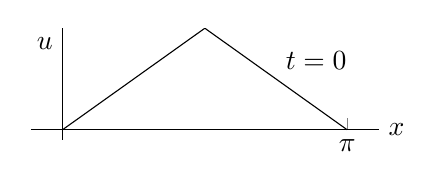
\begin{tikzpicture}
\begin{axis}[height=3cm,width=6cm,axis lines*=middle,xtick={180},ytick={\empty},xticklabels={$\pi$},xlabel={$x$},ylabel={$u$},x label style={at={(current axis.right of origin)},anchor=west},y label style={at={(current axis.above origin)},anchor=north east},y label style={rotate=-90},xmax=200,ymax=3]
\addplot[domain=0:90]{3/90*x};
\addplot[domain=90:180]{3/90*(180-x)}node[pos=0.5,above right]{$t=0$};
\end{axis}
\end{tikzpicture}
\end{subfigure}
%
\begin{subfigure}{1\textwidth}
\centering
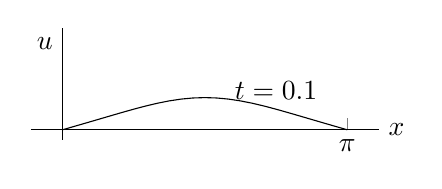
\begin{tikzpicture}
\begin{axis}[height=3cm,width=6cm,axis lines*=middle,xtick={180},ytick={\empty},xticklabels={$\pi$},xlabel={$x$},ylabel={$u$},x label style={at={(current axis.right of origin)},anchor=west},y label style={at={(current axis.above origin)},anchor=north east},y label style={rotate=-90},xmax=200,ymax=3]
\addplot[domain=0:180]{sin(x)*e^(-0.1)-1/9*sin(3*x)*e^(-9*0.1)}node[pos=0.75,above]{$t=0.1$};
\end{axis}
\end{tikzpicture}
\end{subfigure}
%
\begin{subfigure}{1\textwidth}
\centering
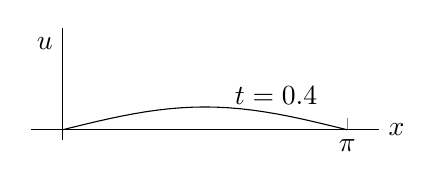
\begin{tikzpicture}
\begin{axis}[height=3cm,width=6cm,axis lines*=middle,xtick={180},ytick={\empty},xticklabels={$\pi$},xlabel={$x$},ylabel={$u$},x label style={at={(current axis.right of origin)},anchor=west},y label style={at={(current axis.above origin)},anchor=north east},y label style={rotate=-90},xmax=200,ymax=3]
\addplot[domain=0:180]{sin(x)*e^(-0.4)-1/9*sin(3*x)*e^(-9*0.4)}node[pos=0.75,above]{$t=0.4$};
\end{axis}
\end{tikzpicture}
\end{subfigure}
%
\begin{subfigure}{1\textwidth}
\centering
\begin{tikzpicture}
\begin{axis}[height=3cm,width=6cm,axis lines*=middle,xtick={180},ytick={\empty},xticklabels={$\pi$},xlabel={$x$},ylabel={$u$},x label style={at={(current axis.right of origin)},anchor=west},y label style={at={(current axis.above origin)},anchor=north east},y label style={rotate=-90},xmax=200,ymax=3]
\addplot[domain=0:180]{sin(x)*e^(-1)-1/9*sin(3*x)*e^(-9*1)}node[pos=0.75,above]{$t=1$};
\end{axis}
\end{tikzpicture}
\end{subfigure}
\caption{مختلف لمحات پر مثال \حوالہ{مثال_جزوی_حراری_الف} کا حل}
\label{شکل_مثال_جزوی_حراری_الف}
\end{figure}
%

\انتہا{مثال}
%========================

\حصہء{سوالات}

%================
\ابتدا{سوال}\quad 
شکل \حوالہ{شکل_مثال_جزوی_حراری_الف}  کا شکل \حوالہ{شکل_سوال_جزوی_شکل_انحراف_الف} کے ساتھ موازنہ کریں۔دونوں میں کیا اہم فرق پایا جاتا ہے۔\\
جواب:\quad شکل \حوالہ{شکل_مثال_جزوی_حراری_الف} غیر ارتعاشی ہے جبکہ مساوات موج کا حل ارتعاشی ہے
\انتہا{سوال}
%======================
\ابتدا{سوال} \quad 
مساوات \حوالہ{مساوات_جزوی_حل_حرارت_ث} میں کسی مخصوص \عددی{n} کے لئے \عددی{K}، \عددی{\sigma} اور \عددی{\rho} کا تنزل پر کیا اثر پایا جاتا ہے؟\\
جواب:\quad \عددی{K} بڑھنے سے تنزل بڑھتی ہے جبکہ \عددی{\sigma} اور \عددی{\rho} کے بڑھنے سے تنزل گھٹتی ہے۔
\انتہا{سوال}
%================
\ابتدا{سوال} \quad 
\عددی{u_1}، \عددی{u_2} اور \عددی{u_3} کا ترسیم  \عددی{B_n=1}، \عددی{c=1} اور \عددی{l=\pi} لیتے ہوئے \عددی{t=0}، \عددی{t=1} اور \عددی{t=2} کے لئے کھینچیں۔
\انتہا{سوال}
%===================
\ابتدا{سوال}\شناخت{سوال_جزوی_حاجز_اطراف}\quad
ایک سلاخ جس کے اطراف مکمل طور حاجز شدہ ہیں  کے سر برقرار \عددی{u(0,t)=U_1} اور \عددی{u(0,l)=U_2} پر رکھے گئے ہیں۔سلاخ کی لمبائی \عددی{l} ہے۔بہت دیر بعد (یعنی \عددی{t\to \infty} پر) سلاخ میں درجہ حرارت \عددی{u_I(x)} دریافت کریں۔ \\
جواب:\quad
$u_I=U_1+(U_2-U_1)\tfrac{x}{l}$
جہاں \عددی{\tfrac{\partial u}{\partial t}=0} سرحدی شرائط کو مطمئن کرتا ہے۔
\انتہا{سوال}
%==================
سوال \حوالہ{سوال_جزوی_سلاخ_الف} تا سوال \حوالہ{سوال_جزوی_سلاخ_ب} میں لوہے کی سلاخ کا درجہ حرارت \عددی{u(x,t)} دریافت کریں۔ سلاخ کی لمبائی \عددی{L=\SI{1}{\meter}} ہے جبکہ لوہے کے مستقل \عددی{K=\SI{73}{\watt\per\meter\per\celsius}}، \عددی{\sigma=\SI{444}{\joule\per\kilo\gram\per\celsius}} اور \عددی{\rho=\SI{7860}{\kilo\gram\per\meter^3}} ہیں۔ سلاخ کا رقبہ عمودی تراش \عددی{\SI{1}{\centi\meter\squared}} ہے جبکہ اس کے سر \عددی{\SI{0}{\celsius}} پر برقرار رکھے گئے ہیں۔ابتدائی درجہ حرارت \عددی{f(x)} ہے۔سلاخ کے اطراف حاجز شدہ ہیں۔

%========================
\ابتدا{سوال}\شناخت{سوال_جزوی_سلاخ_الف}
\begin{align*}
f(x)=
\begin{cases}
x&0<x<\frac{L}{2}\\
L-x&\frac{L}{2}<x<L
\end{cases}
\end{align*}
جواب:\quad
$u=\tfrac{4}{\pi^2}(e^{-\lambda_1^2 t}\sin \pi x-\tfrac{1}{9}e^{-9\lambda_1^2 t}\sin 3\pi x+-\cdots)\quad \quad \lambda_1^2=\tfrac{73\pi^2}{3489840}$
\انتہا{سوال}
%====================
\ابتدا{سوال}\quad
$f(x)=\sin \pi x$\\
جواب:\quad
$u=e^{-\lambda_1^2 t}\sin \pi x\quad \quad \lambda_1^2=\tfrac{73\pi^2}{3489840}$
\انتہا{سوال}
%========================
\ابتدا{سوال}\quad
\begin{align*}
f(x)=
\begin{cases}
x^2&0<x<\frac{L}{2}\\
0&\frac{L}{2}<x<L
\end{cases}
\end{align*}
جواب:\quad
$u=(\tfrac{2}{\pi^2}-\tfrac{4}{\pi^3})e^{-\lambda_1^2t}\sin\pi x+(\tfrac{1}{4\pi}-\tfrac{1}{\pi^3})e^{-4\lambda_1^2t}\sin 2\pi x\cdots \quad \quad \lambda_1^2=\tfrac{73\pi^2}{3489840}$
\انتہا{سوال}
%===================
\ابتدا{سوال}\quad
$f(x)=x(L-x)$\\
جواب:\quad
$u=\tfrac{8}{\pi^3}(e^{-\lambda_1^2t}\sin \pi x+\tfrac{1}{9}e^{-9\lambda_1^2t}\sin 3\pi x+\cdots)\quad \quad \lambda_1^2=\tfrac{73\pi^2}{3489840}$

\انتہا{سوال}
%======================
\ابتدا{سوال}\quad
$f(x)=x(L-x^2)$\\
جواب:\quad
$u=\tfrac{12}{\pi^3}e^{-\lambda_1^2t}\sin \pi x-\tfrac{3}{2\pi^3}e^{-4\lambda_1^2t}\sin 2\pi x\cdots\quad \quad \lambda_1^2=\tfrac{73\pi^2}{3489840}$
\انتہا{سوال}
%======================
\ابتدا{سوال}\شناخت{سوال_جزوی_سلاخ_ب}\quad
$f(x)=x\sin \pi x$\\
جواب:\quad
$u=\tfrac{1}{2}e^{-\lambda_1^2t\sin \pi x-\tfrac{16}{9\pi^2}e^{-4\lambda_1^2t}\sin 2\pi x}\cdots \quad \quad \lambda_1^2=\tfrac{73\pi^2}{3489840}$
\انتہا{سوال}
%======================
\ابتدا{سوال}\شناخت{سوال_جزوی_سلاخ_پ}\quad
ایک سلاخ جس کی لمبائی \عددی{L} ہے  ہر طرف سے (بشمول دونوں سر) حاجز شدہ ہے۔ابتدائی درجہ حرارت \عددی{f(x)} ہے۔طبعی معلومات: سلاخ کے سر سے حراری توانائی کا اخراج سر پر  \عددی{\tfrac{\partial u}{\partial x}} کے راست تناسب ہو گا۔ تصدیق کریں کہ دی گئی  معلومات درج ذیل کے مترادف ہے۔
\begin{align*}
u_x(0,t)=0,\quad u_x(l,t)=0,\quad u(x,0)=f(x)
\end{align*}
علیحدگی متغیرات استعمال کرتے ہوئے درج ذیل حل حاصل کریں
\begin{align*}
u(x,t)=A_0+\sum_{n=1}^{\infty} A_n\cos\frac{n\pi x}{l}e^{-\lambda_n^2 t},\quad \quad \lambda_n=\tfrac{cn\pi}{l}
\end{align*}
جہاں \عددی{A_0} اور \عددی{A_n} مساوات \حوالہ{مساوات_فوریئر_نصف_حلقہ_توسیع_جفت_عددی_سر} سے  درج ذیل ہیں۔
\begin{align*}
A_0=\frac{1}{l}\int_0^l f(x)\dif x,\quad A_n=\frac{2}{l}\int_0^l f(x)\cos \frac{n\pi x}{l}\dif x,\quad \quad n=1,2,\cdots
\end{align*}
\انتہا{سوال}
%======================
\ابتدا{سوال}\quad
سوال \حوالہ{سوال_جزوی_سلاخ_پ} میں \عددی{t\to \infty} پر \عددی{u\to A_0} ملتا ہے۔کیا یہ آپ کے توقع کے مطابق ہے؟
\انتہا{سوال}
%====================
سوال \حوالہ{سوال_جزوی_سلاخ_حاجز_شدہ_الف} تا سوال \حوالہ{سوال_جزوی_سلاخ_حاجز_شدہ_ب} کو سوال \حوالہ{سوال_جزوی_سلاخ_پ} میں دی گئی صورت حال کے لئے حل کریں جہاں  \عددی{l=\pi} اور \عددی{c=1} ہیں۔

%=================
\ابتدا{سوال}\شناخت{سوال_جزوی_سلاخ_حاجز_شدہ_الف}\quad
$f(x)=1$\\
جواب:\quad
$u(x,t)=1$
\انتہا{سوال}
%=====================
\ابتدا{سوال}\quad
$f(x)=x$\\
جواب:\quad
$u=\tfrac{\pi}{2}-\tfrac{4}{\pi}(e^{-t}\cos x+\tfrac{1}{9}e^{-9t}\cos 3x+\tfrac{1}{25}e^{-25t}\cos 5x\cdots)$
\انتہا{سوال}
%=====================
\ابتدا{سوال}\quad
$f(x)=x^2$\\
جواب:\quad
$u=\tfrac{\pi^2}{3}-4(e^{-t}\cos x-\tfrac{1}{4}e^{-4t}\cos 2x+\tfrac{1}{9}e^{-9t}\cos 3x\cdots)$
\انتہا{سوال}
%=====================
\ابتدا{سوال}\quad
\begin{align*}
f(x)=
\begin{cases}
x&0<x<\tfrac{L}{2}\\
L-x&\tfrac{L}{2}<x<L
\end{cases}
\end{align*}
جواب:\quad
$u=\tfrac{\pi}{4}-\tfrac{2}{\pi}(e^{-4t}\cos 2x+\tfrac{1}{9}e^{-36t}\cos 6x+\tfrac{1}{25}e^{-100t}\cos 10x\cdots)$
\انتہا{سوال}
%=====================
\ابتدا{سوال}\شناخت{سوال_جزوی_سلاخ_حاجز_شدہ_ب}\quad
\begin{align*}
f(x)=
\begin{cases}
1&0<x<\tfrac{L}{2}\\
-1&\tfrac{L}{2}<x<L
\end{cases}
\end{align*}
جواب:\quad
$u=\tfrac{4}{\pi}(e^{-t}\cos x-\tfrac{1}{3}e^{-9t}\cos 3x+\tfrac{1}{5}e^{-25t}\cos 5x\cdots)$
\انتہا{سوال}
%=====================
\ابتدا{سوال}\quad 
فرض کریں کہ سوال \حوالہ{سوال_جزوی_حاجز_اطراف} میں ابتدائی درجہ حرارت \عددی{u(x,0)=f(x)} ہے۔ثابت کریں کہ کسی بھی لمحے پر سلاخ میں درجہ حرارت \عددی{u(x,y)=u_I(x)+u_{II}(x,t)} ہو گی جہاں \عددی{u_I} پہلی کی طرح ہے جبکہ \عددی{u_{II}} درج ذیل ہے
\begin{align*}
u_{II}=\sum_{n=1}^{\infty} B_n\sin\frac{n\pi x}{l}e^{-\tfrac{c^2n^2\pi^2}{l^2}t}
\end{align*}
جہاں \عددی{B_n} درج ذیل ہے۔
\begin{align*}
B_n&=\frac{2}{l}\int_0^l [f(x)-u_I(x)]\sin \frac{n\pi x}{l}\dif x\\
&=\frac{2}{l}\int_0^l f(x)\sin \frac{n\pi x}{l}\dif x+\frac{2}{n\pi}[(-1)^nU_2-U_1]
\end{align*}
\انتہا{سوال}
%========================

\حصہ{لامتناہی لمبائی کی سلاخ میں بہاو حرارت}\شناخت{حصہ_جزوی_نصف_لامتناہی_سلاخ}
ہم اطراف سے حاجز شدہ ایسی سلاخ جو دونوں جانب لامتناہی تک لمبی ہو کی صورت میں حراری مساوات
\begin{align}\label{مساوات_جزوی_حراری_لامتناہی_الف}
\frac{\partial u}{\partial t}=c^2\frac{\partial^{\,2}u}{\partial x^2}
\end{align}
پر غور کریں گے۔ایسی صورت میں ہمارے پاس کوئی سرحدی شرط نہیں ہے جبکہ ابتدائی معلومات درج ذیل ہے۔
\begin{align}\label{مساوات_جزوی_حراری_لامتناہی_ب}
u(x,0)=f(x)\quad \quad \quad (-\infty<x<\infty)
\end{align}

اس مسئلے کو حل کرنے کی خاطر ہم مساوات \حوالہ{مساوات_جزوی_حراری_لامتناہی_الف} میں \عددی{u(x,t)=F(x)G(t)} پر کرتے ہوئے درج ذیل دو عدد سادہ تفرقی مساوات حاصل کرتے ہیں
\begin{align}
F''+p^2F&=0\label{مساوات_جزوی_حراری_لامتناہی_پ}\\
\dot{G}+c^2p^2G&=0\label{مساوات_جزوی_حراری_لامتناہی_ت}
\end{align} 
جن کا موازنہ مساوات \حوالہ{مساوات_جزوی_حل_حرارت_پ} اور مساوات \حوالہ{مساوات_جزوی_حل_حرارت_ت} کے ساتھ کرتے ہوئے درج ذیل حل لکھے جا سکتے ہیں
\begin{align*}
F(x)=A\cos px+B\sin px\quad \text{اور}\quad G(t)=e^{-c^2p^2t}
\end{align*}
جہاں \عددی{A} اور \عددی{B} اختیاری  مستقل ہیں۔اس طرح مساوات \حوالہ{مساوات_جزوی_حراری_لامتناہی_الف} کا حل
\begin{align}\label{مساوات_جزوی_حراری_لامتناہی_ٹ}
u(x,t;p)=FG=(A\cos px+B\sin px)e^{-c^2p^2t}
\end{align}
ہو گا۔[گزشتہ حصے کی طرح یہاں بھی علیحدگی کا مستقل \عددی{k} منفی لینا ہو گا یعنی \عددی{k=-p^2} چونکہ مثبت \عددی{k} کی صورت میں مساوات \حوالہ{مساوات_جزوی_حراری_لامتناہی_ٹ} میں مسلسل بڑھتی قوت نمائی تفاعل پیدا ہوتا ہے جس کا کوئی طبعی مطلب ممکن نہیں ہے۔]

مساوات \حوالہ{مساوات_جزوی_حراری_لامتناہی_ٹ} کی تفاعل میں \عددی{p} کی قیمتوں کو کسی مستقل عدد کا ضربی  لے کر ان تفاعل کی تسلسل لکھی جا سکتی ہے لیکن ایسی تسلسل  لمحہ \عددی{t=0} پر \عددی{x} کے لحاظ سے دوری ہو گی لیکن \عددی{f(x)} غیر دوری ہے۔یوں فطری بات ہے کہ ہم فوریئر تسلسل کی بجائے فوریئر تکمل کی طرف رجحان کریں۔

چونکہ مساوات \حوالہ{مساوات_جزوی_حراری_لامتناہی_ٹ} میں \عددی{A} اور \عددی{B} اختیاری مستقل ہیں لہٰذا  ہم انہیں \عددی{p} کے تفاعل \عددی{A=A(p)} اور \عددی{B=B(p)} تصور کر سکتے ہیں۔چونکہ حراری مساوات خطی اور ہم جنسی ہے لہٰذا
\begin{align}\label{مساوات_جزوی_حراری_لامتناہی_ث}
u(x,t)=\int_0^{\infty}u(x,t;p)\dif p=\int_0^{\infty}[A(p)\cos px+B(p)\sin px]e^{-c^2p^2t}\dif p
\end{align}
مساوات \حوالہ{مساوات_جزوی_حراری_لامتناہی_الف} کا حل ہو گا بشرطیکہ یہ تکمل موجود ہو اور یہ دو مرتبہ \عددی{x} کے ساتھ اور ایک مرتبہ \عددی{t} کے ساتھ قابل تفرق ہو۔

مساوات \حوالہ{مساوات_جزوی_حراری_لامتناہی_ث} اور ابتدائی معلومات مساوات \حوالہ{مساوات_جزوی_حراری_لامتناہی_ب} سے درج ذیل لکھا جا سکتا ہے۔
\begin{align}\label{مساوات_جزوی_حراری_لامتناہی_ج}
u(x,0)=\int_0^{\infty}[A(p)\cos px+B(p)\sin px]\dif p=f(x)
\end{align}
مساوات \حوالہ{مساوات_فوریئر_تکمل_ت} اور مساوات \حوالہ{مساوات_فوریئر_تکمل_ٹ} استعمال کرتے ہوئے یوں درج ذیل حاصل ہوتا ہے۔
\begin{align}\label{مساوات_جزوی_حراری_لامتناہی_چ}
A(p)=\frac{1}{\pi}\int_{-\infty}^{\infty} f(v)\cos pv\,\dif v,\quad B(p)=\frac{1}{\pi}\int_{-\infty}^{\infty} f(v)\sin pv\,\dif v
\end{align}
صفحہ \حوالہصفحہ{مساوات_فوریئر_بدل_الف} پر مساوات \حوالہ{مساوات_فوریئر_بدل_الف} کے تحت اس تکمل کو
\begin{align*}
u(x,0)=\frac{1}{\pi}\int_{0}^{\infty} \big[\int_{-\infty}^{\infty} f(v)\cos(px-pv)\,\dif v\big]\dif p
\end{align*}
لکھا جا سکتا ہے لہٰذا مساوات \حوالہ{مساوات_جزوی_حراری_لامتناہی_ث} درج ذیل صورت اختیار کرتی ہے۔
\begin{align*}
u(x,t)=\frac{1}{\pi}\int_0^{\infty}\big[\int_{-\infty}^{\infty}f(v)\cos (px-pv)e^{-c^2p^2t}\,\dif v\big]\dif p
\end{align*}
یہ فرض کرتے ہوئے کہ اس دوہرا تکمل کی ترتیب بدلی جا سکتی ہے ہم اس کو درج ذیل لکھ سکتے ہیں۔
\begin{align}\label{مساوات_جزوی_حراری_لامتناہی_ح}
u(x,t)=\frac{1}{\pi}\int_{-\infty}^{\infty} f(v) \big[\int_0^{\infty}e^{-c^2p^2t}\cos(px-pv)\,\dif p\big]\dif v
\end{align}
اندرونی تکمل کو درج ذیل کلیہ کی مدد سے حل کیا جا سکتا ہے۔
\begin{align}\label{مساوات_جزوی_حراری_لامتناہی_خ}
\int_0^{\infty}e^{-s^2}\cos 2bs\,\dif s=\frac{\sqrt{\pi}}{2}e^{-b^2}
\end{align}
مساوات \حوالہ{مساوات_جزوی_حراری_لامتناہی_خ} میں نیا متغیرہ \عددی{p} متعارف کرتے ہوئے \عددی{s=cp\sqrt{t}} لکھ کر اور
\begin{align*}
b=\frac{x-v}{2c\sqrt{t}}
\end{align*}
لیتے ہوئے مساوات \حوالہ{مساوات_جزوی_حراری_لامتناہی_خ} درج ذیل صورت اختیار کرتی ہے
\begin{align*}
\int_0^{\infty}e^{-c^2p^2t}\cos (px-pv)\,\dif p=\frac{\sqrt{\pi}}{2c\sqrt{t}}e^{-\tfrac{(x-v)^2}{4c^2t}}
\end{align*}
جس کو مساوات \حوالہ{مساوات_جزوی_حراری_لامتناہی_ح} میں پر کرتے ہوئے 
\begin{align}\label{مساوات_جزوی_لامتناہی_سلاخ_حل_الف}
u(x,t)=\frac{1}{2c\sqrt{\pi t}}\int_{-\infty}^{\infty}f(v)e^{-\frac{(x-v)^2}{4c^2t}}\,\dif v
\end{align}
ملتا ہے۔آخر میں ہم تکمل کا متغیرہ \عددی{z=\tfrac{v-x}{2c\sqrt{t}}} متعارف  کرتے ہوئے 
\begin{align}\label{مساوات_جزوی_لامتناہی_سلاخ_حل_ب}
u(x,t)=\frac{1}{\sqrt{\pi}}\int_{-\infty}^{\infty} f(x+2cz\sqrt{t})e^{-z^2}\,\dif z
\end{align}
حاصل کرتے ہیں۔ تمام \عددی{x} کے لئے محدود \عددی{f(x)}  اور ہر محدود وقفہ پر قابل تکمل \عددی{f(x)} کی صورت میں  یہ ثابت کیا جا سکتا ہے کہ  مساوات \حوالہ{مساوات_جزوی_لامتناہی_سلاخ_حل_الف} اور مساوات \حوالہ{مساوات_جزوی_لامتناہی_سلاخ_حل_ب} دونوں  مساوات \حوالہ{مساوات_جزوی_حراری_لامتناہی_الف} اور مساوات \حوالہ{مساوات_جزوی_حراری_لامتناہی_ب} کو مطمئن کرتے ہیں لہٰذا یہ موجودہ مسئلے کا حل ہیں۔

%=======================
\ابتدا{مثال}\شناخت{مثال_جزوی_لامتناہی_سلاخ}\quad لامتناہی لمبائی کی سلاخ میں درجہ حرارت\\
لامتناہی لمبائی کی سلاخ میں ابتدائی درجہ حرارت درج ذیل ہے (شکل \حوالہ{مثال_جزوی_لامتناہی_سلاخ})۔
\begin{align*}
f(x)=
\begin{cases}
U_0=\text{مستقل}& \abs{x}<1\\
0&\abs{x}>1
\end{cases}
\end{align*}
%
\begin{figure}
\centering
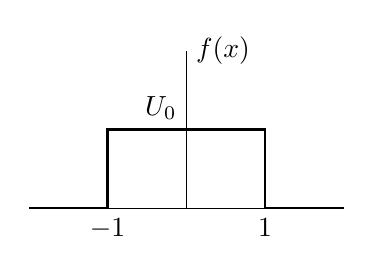
\begin{tikzpicture}
\draw(-2,0)--(2,0);
\draw(0,0)--(0,2)node[right]{$f(x)$};
\draw[thick](-2,0)--(-1,0)node[below]{$-1$}--(-1,1)--(1,1)--(1,0)node[below]{$1$}--(2,0);
\draw(0,1)node[above left]{$U_0$};
\end{tikzpicture}
\caption{ابتدائی درجہ حرارت (مثال \حوالہ{مثال_جزوی_لامتناہی_سلاخ})}
\label{شکل_مثال_جزوی_لامتناہی_سلاخ}
\end{figure}
مساوات \حوالہ{مساوات_جزوی_لامتناہی_سلاخ_حل_الف} سے 
\begin{align*}
u(x,t)=\frac{U_0}{2c\sqrt{\pi t}}\int_{-1}^{1} e^{-\tfrac{(x-v)^2}{4c^2t}}\,\dif v
\end{align*}
لکھتے ہیں۔تکمل کا نیا متغیرہ \عددی{z=\tfrac{v-x}{2c\sqrt{t}}} استعمال کرتے ہوئے \عددی{-1} تا \عددی{1} پر \عددی{v} کا تکمل \عددی{\tfrac{-1-x}{2c\sqrt{t}}} تا \عددی{\tfrac{1-x}{2c\sqrt{t}}}  پر \عددی{z} کے تکمل  میں تبدیل ہو گا یعنی؛
\begin{align}\label{مساوات_جزوی_حل_مثال_جزوی_لامتناہی_سلاخ}
u(x,t)=\frac{U_0}{\sqrt{\pi}}\int\limits_{\tfrac{-1-x}{2c\sqrt{t}}}^{\tfrac{1-x}{2c\sqrt{t}}} e^{-z^2}\, \dif z \quad \quad (z>0)
\end{align}
اس تکمل کو بنیادی تفاعل کی صورت میں حاصل نہیں کیا جا سکتا ہے البتہ اس کو \اصطلاح{تفاعل خلل}\فرہنگ{خلل!تفاعل}\فرہنگ{تفاعل!خلل}\حاشیہب{error function}\فرہنگ{error!function} کی صورت میں لکھا جا سکتا ہے۔ شکل \حوالہ{شکل_مثال_جزوی_لامتناہی_سلاخ_حل} میں \عددی{u(x,t)} کو \عددی{U_0=\SI{100}{\celsius}}، \عددی{c^2=\SI{1}{\centi\meter\squared\per\second}} کے لئے لمحات \عددی{t=\tfrac{1}{8},\tfrac{1}{2},1,2,8} پر دکھایا گیا ہے۔
\begin{figure}
\centering
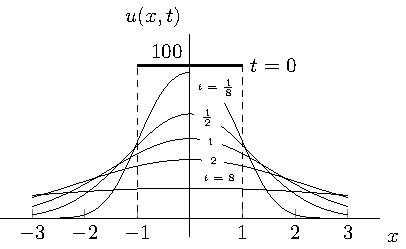
\includegraphics{figInfiniteBarHeatProblem}
\caption{حل $u(x,t)$ برائے مثال \حوالہ{مثال_جزوی_لامتناہی_سلاخ}}
\label{شکل_مثال_جزوی_لامتناہی_سلاخ_حل}
\end{figure}
\انتہا{مثال}
%=======================

\حصہء{سوالات}
%====================
\ابتدا{سوال}\quad
نقطہ \عددی{x=0.5,1,1.5} پر مثال \حوالہ{مثال_جزوی_لامتناہی_سلاخ} میں \عددی{U_0=\SI{100}{\celsius}} اور \عددی{c^2=\SI{1}{\meter\squared\per\second}} لے کر حاصل کردہ درجہ حرارت \عددی{u(x,t)} کی ترسیم مختلف لمحات پر  کھینچیں۔کیا جوابات آپ کی سوچ کے مطابق ہیں؟
\انتہا{سوال}
%=======================
\اصطلاح{تفاعل خلل} درج ذیل تکمل کو کہتے ہیں
\begin{align*}
\erf x =\frac{2}{\sqrt{\pi}}\int_0^x e^{-w^2}\,\dif w
\end{align*} 
جو انجینئری میں کلیدی کردار ادا کرتا ہے۔اس سے واقفیت  پیدا کرنے کی خاطر سوال \حوالہ{سوال_جزوی_تفاعل_خلل_الف} تا سوال \حوالہ{سوال_جزوی_تفاعل_خلل_ب} حل کریں۔

%======================
\ابتدا{سوال}\شناخت{سوال_جزوی_تفاعل_خلل_الف}\quad 
تصدیق کریں کہ تفاعل خلل طاق ہے۔
\انتہا{سوال}
%=====================
\ابتدا{سوال}\quad درج ذیل ثابت کریں۔\\
 $\int_a^be^{-w^2}\,\dif w=\frac{\sqrt{\pi}}{2}(\erf b-\erf a),\quad \int_{-b}^be^{-w^2}\,\dif w=\sqrt{\pi}\erf b$
\انتہا{سوال}
%======================
\ابتدا{سوال}\شناخت{سوال_جزوی_قوس_جرس}\quad
قلم و کاغذ سے متکمل \عددی{e^{-w^2}} کی قیمتوں کا جدول بناتے ہوئے اس کی ترسیم کھینچیں جو \اصطلاح{قوس جرس}\فرہنگ{قوس جرس}\فرہنگ{جرس!قوس}\حاشیہب{bell curve}\فرہنگ{bell curve} کہلاتی ہے۔  
\انتہا{سوال}
%======================
\ابتدا{سوال}\quad
قوس جرس (جس کو آپ نے سوال \حوالہ{سوال_جزوی_قوس_جرس} میں حاصل کیا) کے نیچے رقبہ معلوم کرتے ہوئے \عددی{\erf x} کا جدول \عددی{x=0,0.2,0.4,\cdots ,1,1.5,2} کے لئے حاصل کریں۔قوس جرس پر افقی اور انتصابی لکیریں کھینچ کر قوس کے نیچے مکعب گن کر رقبہ حاصل کیا جا سکتا ہے۔\\
جوابات:\quad نقطہ اعشاریہ کے بعد صرف دو اعداد لیتے ہوئے۔\\
$0.00, 0.22, 0.43, 0.60, 0.74, 0.84,0.97,1.00\quad $
\انتہا{سوال}
%======================
\ابتدا{سوال}\quad تفاعل خلل کی متکمل \عددی{e^{-w^2}} کی مکلارن تسلسل حاصل کریں۔اس تسلسل کا تکمل لے کر تفاعل خلل \عددی{\erf x} کی مکلارن تسلسل دریافت کریں۔\\
جواب:\quad
$\erf x=\tfrac{2}{\sqrt{\pi}}(x-\tfrac{x^3}{3}+\tfrac{x^5}{10}-\tfrac{x^7}{42}+\tfrac{x^9}{216}\cdots)$
\انتہا{سوال}
%======================
\ابتدا{سوال}\quad 
مساوات \حوالہ{مساوات_جزوی_حل_مثال_جزوی_لامتناہی_سلاخ} سے درج ذیل صورت  حاصل کریں۔
\begin{align*}
u(x,t)=\frac{U_0}{2}\big[\erf \frac{1-x}{2c\sqrt{t}}+\erf \frac{1+x}{2c\sqrt{t}}\big]\quad \quad (t>0)
\end{align*}
\انتہا{سوال}
%================
\ابتدا{سوال}\شناخت{سوال_جزوی_سلاخ_سیڑھی}\quad اگر \عددی{x>0} کی صورت میں \عددی{f(x)=1} اور \عددی{x<0} کی صورت میں \عددی{f(x)=0} ہو تب تصدیق کریں کہ مساوات \حوالہ{مساوات_جزوی_لامتناہی_سلاخ_حل_ب} سے درج ذیل حاصل ہو گا۔
\begin{align*}
u(x,t)=\frac{1}{\sqrt{\pi}}\int\limits_{-\tfrac{x}{2c\sqrt{t}}}^{\infty} e^{-z^2}\,\dif z\quad \quad (t>0)
\end{align*}
\انتہا{سوال}
%===============
\ابتدا{سوال}\شناخت{سوال_جزوی_تفاعل_خلل_ب}\quad
چونکہ \عددی{\erf \infty=1} ہے لہٰذا سوال \حوالہ{سوال_جزوی_سلاخ_سیڑھی} سے درج ذیل حاصل کریں۔
\begin{align*}
u(x,t)=\frac{1}{2}+\frac{1}{2}\erf \frac{x}{2c\sqrt{t}}
\end{align*}
\انتہا{سوال}
%====================
\ابتدا{سوال}\شناخت{سوال_جزوی_نصف_لامتناہی}\quad
نصف لامتناہی لمبی سلاخ (\عددی{0} تا \عددی{\infty}) کے \عددی{x=0} پر سر کو صفر درجہ پر رکھا گیا ہے جبکہ اس کی ابتدائی درجہ حرارت \عددی{f(x)} ہے۔ثابت کریں کہ اس مسئلہ کا حل درج ذیل ہے جہاں \عددی{\tau=2c\sqrt{t}} ہے۔
\begin{align}\label{مساوات_جزوی_لامتناہی_سلاخ_حل_پ}
u(x,t)=\frac{1}{\sqrt{\pi}}\big[\int_{-\tfrac{x}{\tau}}^{\infty} f(x+\tau w)e^{-w^2}\,\dif w-\int_{\tfrac{x}{\tau}}^{\infty} f(-x+\tau w)e^{-w^2}\,\dif w\big]
\end{align}

\انتہا{سوال}
%==================
\ابتدا{سوال}\quad \عددی{f(v)} کو طاق تصور کرتے ہوئے مساوات \حوالہ{مساوات_جزوی_لامتناہی_سلاخ_حل_الف} سے مساوات \حوالہ{مساوات_جزوی_لامتناہی_سلاخ_حل_پ} حاصل کریں۔ 
\انتہا{سوال}
%======================
\ابتدا{سوال}\شناخت{سوال_جزوی_اکائی_تفاعل}\quad \عددی{f(x)=1}  لیتے ہوئے ثابت کریں کہ سوال \حوالہ{سوال_جزوی_نصف_لامتناہی} میں درج ذیل حل حاصل ہو گا۔
\begin{align*} 
u(x,t)=\frac{2}{\sqrt{\pi}}\int_0^{\tfrac{x}{\tau}} e^{-w^2}\,\dif w=\erf \frac{x}{2c\sqrt{t}}\quad \quad (t>0)
\end{align*}
\انتہا{سوال}
%========================
\ابتدا{سوال}\quad درج ذیل ابتدائی معلومات کی صورت میں مساوات \حوالہ{مساوات_جزوی_لامتناہی_سلاخ_حل_پ} کیا صورت اختیار کرے گی۔
\begin{align*}
f(x)=
\begin{cases}
1& a<x<b \quad \quad (a>0)\\
0& \text{\RL{باقی جگہوں پر}}
\end{cases}
\end{align*}
جواب:\quad
\begin{align*}
\frac{1}{\sqrt{\pi}}\int\limits_{\tfrac{a-x}{\tau}}^{\tfrac{b-x}{\tau}}e^{-w^2}\,\dif w-\frac{1}{\pi}\int\limits_{\tfrac{a+x}{\tau}}^{\tfrac{b+x}{\tau}}e^{-w^2}\,\dif w
\end{align*}
\انتہا{سوال}
%==================
\ابتدا{سوال}\quad
\عددی{x>0} پر \عددی{f(x)=1} اور \عددی{x<0} پر \عددی{f(x)=-1} لیتے ہوئے مساوات \حوالہ{مساوات_جزوی_لامتناہی_سلاخ_حل_الف} یا مساوات \حوالہ{مساوات_جزوی_لامتناہی_سلاخ_حل_ب} کی استعمال سے سوال \حوالہ{سوال_جزوی_اکائی_تفاعل} کا نتیجہ حاصل کریں۔ 
\انتہا{سوال}
%====================
\ابتدا{سوال}\quad ثابت کریں کہ سوال \حوالہ{مساوات_جزوی_لامتناہی_سلاخ_حل_الف} میں کوئی دو نقطے کا ایک ہی درجہ حرارت تک پہنچنے کے لئے درکار وقت ان نقطوں کا سرحد \عددی{x=0} سے فاصلہ کے مربع کے راست تناسب ہو گا۔  
\انتہا{سوال}
%=====================

\حصہ{نمونہ کشی: ارتعاش پذیر جھلی۔ دو ابعادی مساوات موج}\شناخت{حصہ_جزوی_ارتعاش_جھلی}
ارتعاش کی میدان میں ایک اور اہم مسئلے کے طور پر تننی ہوئی جھلی، مثلاً طبل پر چڑھا ہوا چمڑے کا پردہ، کی ارتعاش پر غور کرتے ہیں۔آپ دیکھیں گے کہ موجودہ تجزیہ حصہ \حوالہ{حصہ_جزوی_ارتعاش_تار} میں ارتعاش تار کی مانند ہو گا۔ 

ہم درج ذیل فرض کرتے  ہیں۔

\موٹا{(الف)}\quad اکائی رقبہ پر جھلی کی کمیت یکساں ہے (ہم جنسی جھلی)۔ جھلی مکمل لچکدار اور اتنی باریک ہے کہ مڑنے کے خلاف مزاحمت فراہم نہیں کرتی ہے۔\\
\موٹا{(ب)}\quad جھلی کو تان کر، اس کی پوری سرحد سے \عددی{xy} مستوی میں باندھا گیا ہے۔ جھلی میں ہر نقطہ  پر اور ہر رخ  فی اکائی لمبائی تناو \عددی{T} یکساں ہے جو ارتعاش کے دوران تبدیل نہیں ہوتی۔\\
\موٹا{(پ)} \quad حرکت کے دوران جھلی کی انحراف \عددی{u(x,y,t)}، جھلی کی جسامت کے لحاظ سے  کم ہے اور تمام زاویہ میلان چھوٹے ہیں۔      

اگرچہ حقیقت میں ان مفروضوں پر مکمل طور پورا اترنا ممکن نہیں ہے، پتلی جھلی کی قلیل عرضی لرزش ان مفروضوں پر تقریباً پورا اترتی ہیں۔

جھلی کی حرکت کی جزوی تفرقی مساوات حاصل کرنے کی خاطر ہم جھلی کے ایک چھوٹے ٹکڑے پر عمل کرنے والی قوتوں پر غور کرتے ہیں (شکل \حوالہ{شکل_جزوی_ارتعاش_پذیر_جھلی})۔چونکہ جھلی کی انحراف اور زاویہ میلان چھوٹے ہیں لہٰذا اس ٹکڑے کے اطراف کی لمبائی تقریباً \عددی{\Delta x} اور \عددی{\Delta y} ہو گی۔اکائی لمبائی پر قوت کو تناو \عددی{T} کہتے ہیں لہٰذا اس ٹکڑے کے اطراف پر قوت
 \عددی{T\Delta x} اور \عددی{T\Delta y} عمل کرے گی۔ چونکہ جھلی مکمل لچکدار ہے لہٰذا یہ قوتیں جھلی کی مماسی ہوں گی۔

\begin{figure}
\centering
\begin{subfigure}{1\textwidth}
\centering
\begin{tikzpicture}
\draw(0,0)--(4,0);
\draw(0,0)--++(0,3);
\draw(0.5,1.5) to [out=-90,in=180](2,0.25) to [out=0,in=-90] (4,1.5) to [out=90,in=0] (3,3)node[above]{\RL{جھلی کی سرحد}} to [out=180,in=90](0.5,1.5);
\draw[thick,fill=gray!50!white] (2,1)--++(1,0)--++(0,1)--++(-1,0)--++(0,-1);
\draw[dashed](2,1)--++(0,-1)node[below]{$x$};
\draw[dashed](3,1)--++(0,-1)node[below]{$x+\Delta x$};
\draw[dashed](2,1)--++(-2,0)node[left]{$y$};
\draw[dashed](2,2)--++(-2,0)node[left]{$y+\Delta y$};
\end{tikzpicture}
\end{subfigure}
\begin{subfigure}{0.5\textwidth}
\centering
\begin{tikzpicture}[x={(1cm,-0.2cm)},y={(0.5cm,0.5cm)},z={(0cm,1cm)}]
\pgfmathsetmacro{\angA}{30}
\pgfmathsetmacro{\angB}{-170}
\pgfmathsetmacro{\angC}{70}
\pgfmathsetmacro{\angD}{-150}
\pgfmathsetmacro{\kdy}{2*tan(\angA)}
\pgfmathsetmacro{\angX}{atan(-0.2/1)}
\pgfmathsetmacro{\angY}{atan(0.5/0.5)}
\pgfmathsetmacro{\iX}{1}
\pgfmathsetmacro{\iY}{1}
\pgfmathsetmacro{\iZ}{1.5}
%
\draw(0,0,0)--++(4,0,0);
\draw(0,0)--++(0,2.5,0);
\draw(0,0)--++(0,0,1);
%
\draw[thick,name path=kL](\iX,\iY,\iZ)coordinate(kA) to [out=\angA,in=\angB]++(2,0,1)coordinate(kB)to [out=\angC,in=\angD]++(0,1,0)coordinate(kC);
\draw(kC) to [out=\angB,in=\angA]++(-2,0,-1)coordinate(kD) to [out=\angD,in=\angC]++(0,-1,0);
%
\draw[dashed](kA)--++(0,0,-\iZ)coordinate(kkA);
\draw[dashed](kB)--++(0,0,-\iZ-1)coordinate(kkB);
\draw[dashed](kC)--++(0,0,-\iZ-1)coordinate(kkC);
\draw[dashed] (\iX,\iY+1,0)coordinate(kkD)--++(0,0,\iZ-0.25);
%
\draw[dashed,fill=gray!50!white] (kkA)--(kkB)--(kkC)--(kkD)--(kkA);
\draw[dashed](kkA)--++(0,-\iY,0)node[shift={(0,-0.3,0),rotate={\angX}},font=\scriptsize,solid]{$x$};
\draw[dashed](kkB)--++(0,-\iY,0)node[shift={(0,-0.3,0)},rotate={\angX},font=\scriptsize,solid]{$x+\Delta x$};
\draw[dashed](kkA)--++(-\iX,0,0)node[shift={(-0.2,0,0)},rotate={\angX},font=\scriptsize,solid]{$y$};
\draw[dashed](kkD)--++(-\iX,0,0)node[shift={(-0.5,0,0)},rotate={\angX},font=\scriptsize,solid]{$y+\Delta y$};
%
\draw[-latex] ($(kB)!0.5!(kC)$)++(0,0,0.1)coordinate(kTBC)--++(40:1.5)node[above]{$T\Delta y$};
\draw[dashed] ($(kB)!0.5!(kC)$)++(0,0,0.1)--++(1.2,0,0);
\draw[-stealth]([shift={(0:0.8)}]kTBC) arc (0:40:0.8);
\draw(kTBC)++(20:1.1)node[]{$\beta$};
%
\draw[-latex] ($(kA)!0.5!(kD)$)++(0,0,0.1)coordinate(kTAD)--++(40:-1.5)node[left]{$T\Delta y$};
\draw[dashed] ($(kA)!0.5!(kD)$)++(0,0,0.1)--++(-1.2,0,0);
\draw[-stealth]([shift={(180:0.8)}]kTAD) arc (180:220:0.8);
\draw(kTAD)++(20:-1.1)node[]{$\alpha$};
%
\draw[-latex] ($(kA)!0.5!(kB)$)++(0,0,0.1)coordinate(kTAB)--++(0,-0.5,-0.2)node[right]{$T\Delta x$};
\draw[-latex] ($(kC)!0.5!(kD)$)++(0,0,0.1)coordinate(kTAB)--++(0,0.6,0)node[above]{$T\Delta x$};
\end{tikzpicture}
\end{subfigure}%
\begin{subfigure}{0.5\textwidth}
\centering
\begin{tikzpicture}
\draw(-1,0)--(3,0);
\draw[thick](0,1.5) to [out=40,in=-170]++(2,1)coordinate(kR);
\draw[dashed](0,1.5)--(0,0)node[below]{$x$};
\draw[dashed](0,1.5)--++(-1,0);
\draw[dashed](kR)--++(0,-2.5)node[below]{$x+\Delta x$};
\draw[-latex](0,1.5)node[ocirc]{}--++(40:-1.2)node[left]{$T\Delta y$};
\draw[-stealth]([shift={(180:0.5)}]0,1.5) arc (180:220:0.5);
\draw(0,1.5)++(20:-0.8)node[]{$\alpha$};
%
\draw[dashed](kR)--++(1,0);
\draw[-latex](kR)node[ocirc]{}--++(30:1.2)node[right]{$T\Delta y$};
\draw[-stealth]([shift={(0:0.5)}]kR) arc (0:30:0.5);
\draw(kR)++(15:0.8)node[]{$\beta$};
\end{tikzpicture}
\end{subfigure}%
\caption{ارتعاش پذیر جھلی}
\label{شکل_جزوی_ارتعاش_پذیر_جھلی}
\end{figure}
ہم پہلے قوتوں کی افقی اجزاء پر غور کرتے ہیں۔اطراف پر قوت کو زاویہ میلان کی کوسائن سے ضرب دینے سے ان کی افقی جزو حاصل ہو گی۔چونکہ زاویہ میلان چھوٹے ہیں لہٰذا ان کی کوسائن تقریباً اکائی \عددی{(1)} کے برابر ہوں گے۔یوں مخالف کناروں پر تقریباً برابر قوتیں پائی جائیں گی۔یوں افقی رخ جھلی کی حرکت قابل نظر انداز ہو گی لہٰذا ہم جھلی کی حرکت کو عرضی حرکت تصور کرتے ہیں یعنی جھلی صرف اوپر نیچے حرکت کرتی ہے۔

اس ٹکڑے کی کناروں پر کھڑی رخ (\عددی{yu} سطح کی متوازی) قوتوں کے اجزاء\حاشیہد{دھیان رہے کہ کنارے پر چلتے ہوئے زاویہ میلان تبدیل ہو گا۔\عددی{\alpha} اور \عددی{\beta} زیر غور کنارے کے کسی موزوں نقطہ پر زاویہ میلان ہوں گے۔} 
\begin{align*}
T\Delta y\,\sin \beta\quad \text{اور}\quad -T\Delta y\,\sin \alpha
\end{align*} 
ہوں گے جہاں منفی علامت نیچے رخ کو ظاہر کرتی ہے۔چونکہ زاویہ میلان چھوٹے ہیں ہم ان کے \عددی{\sin} کی جگہ ان کے \عددی{\tan}  استعمال\حاشیہد{چھوٹے زاویہ \عددی{\theta} کا \عددی{\sin \theta \approx \theta\approx \tan \theta} ہوتا ہے۔} کر سکتے ہیں۔یوں ان دو عدد قوتوں کا مجموعہ
\begin{gather}
\begin{aligned}\label{مساوات_جزوی_قوت_کنارہ_الف}
T\Delta y(\sin \beta-\sin \alpha)& \approx T\Delta y(\tan \beta-\tan \alpha)\\
&=T\Delta y[u_x(x+\Delta x,y_1)-u_x(x,y_2)]
\end{aligned}
\end{gather}
ہو گا جہاں زیر نوشت میں \عددی{x} اور \عددی{y} جزوی تفرق کو ظاہر کرتی ہیں جبکہ \عددی{y} اور \عددی{y+\Delta y} کے درمیان  \عددی{y_1} اور \عددی{y_2}  کوئی نقطے ہیں۔اسی طرح ٹکڑے کے باقی دو کناروں پر قوتوں کے انتصابی اجزاء کا مجموعہ  
\begin{align}\label{مساوات_جزوی_قوت_کنارہ_ب}
T\Delta x[u_y(x_1,y+\Delta y)-u_y(x_2,y)]
\end{align}
ہو گا جہاں \عددی{x} اور \عددی{x+\Delta x} کے درمیان \عددی{x_1} اور \عددی{x_2} کوئی نقطے ہیں۔

نیوٹن کے دوسرے قانون کے تحت مساوات \حوالہ{مساوات_جزوی_قوت_کنارہ_الف} اور مساوات \حوالہ{مساوات_جزوی_قوت_کنارہ_ب} میں دی گئی  قوتوں کا مجموعہ جھلی کے ٹکڑے کی کمیت \عددی{\rho \Delta A} ضرب اسراع \عددی{\tfrac{\partial^{\,2}u}{\partial t^2}} کے برابر ہو گا۔ یہاں بلا انحراف فی اکائی رقبہ جھلی کی کمیت \عددی{\rho} ہے جبکہ بلا انحراف ٹکڑے کا رقبہ \عددی{\Delta A=\Delta x\Delta y} ہے۔یوں
\begin{align*}
\rho\Delta x\Delta y\frac{\partial^{\,2}u}{\partial t^2}=T\Delta y[u_x(x+\Delta x,y_1)-u_x(x,y_2)]+T\Delta x[u_y(x_1,y+\Delta y)-u_y(x_2,y)]
\end{align*}
ہو گا جہاں بائیں ہاتھ تفرق ٹکڑے کے کسی موزوں نقطہ \عددی{(\tilde{x},\tilde{y})} پر حاصل کیا جائے گا۔\عددی{\rho \Delta x\Delta y} سے دونوں اطراف کو تقسیم کرتے ہیں۔
\begin{align*}
\frac{\partial^{\,2}u}{\partial t^2}=\frac{T}{\rho}\big[\frac{u_x(x+\Delta x,y_1)-u_x(x,y_2)}{\Delta x}+\frac{u_y(x_1,y+\Delta y)-u_y(x_2,y)}{\Delta y}\big]
\end{align*}
\عددی{\Delta x} اور \عددی{\Delta y} کو صفر کے قریب تر کرتے ہوئے درج ذیل جزوی تفرقی مساوات حاصل ہو گی
\begin{align}\label{مساوات_جزوی_دو_ابعادی_مساوات_موج_الف}
\frac{\partial^{\,2}u}{\partial t^2}=c^2\left(\frac{\partial^{\,2}u}{\partial x^2}+\frac{\partial^{\,2}u}{\partial y^2}\right)\quad \quad \quad c^2=\frac{T}{\rho}
\end{align}
جس کو \اصطلاح{دو ابعادی مساوات موج}\فرہنگ{موج!دو ابعادی مساوات}\حاشیہب{two dimensional wave equation}\فرہنگ{wave!two dimensional equation} کہتے ہیں۔قوسین میں بند \عددی{u} کا  لاپلاسی \عددی{\nabla^{\,2}u} ہے (حصہ \حوالہ{حصہ_الاحصاء_ڈھلوان}) لہٰذا مساوات \حوالہ{مساوات_جزوی_دو_ابعادی_مساوات_موج_الف} کو درج ذیل لکھا جا سکتا ہے۔
\begin{align}\label{مساوات_جزوی_دو_ابعادی_مساوات_موج_ب}
\frac{\partial^{\,2}u}{\partial t^2}=c^2\nabla^{\,2}u
\end{align}

%=================
\حصہ{مستطیل جھلی}
ارتعاش پذیر جھلی کے مسئلے کو حل کرنے کی خاطر  ہمیں درج ذیل دو ابعادی مساوات موج کا حل \عددی{u(x,y,t)} تلاش کرنا ہو گا
\begin{align}\label{مساوات_جزوی_مستطیل_جھلی_الف}
\frac{\partial^{\,2}u}{\partial t^2}=c^2\left(\frac{\partial^{\,2}u}{\partial x^2}+\frac{\partial^{\,2}u}{\partial y^2}\right)
\end{align}
جو تمام \عددی{t\ge 0} کے لئے پوری سرحد پر سرحدی شرط
\begin{align}\label{مساوات_جزوی_مستطیل_جھلی_ب}
u=0
\end{align}
اور دو عدد ابتدائی شرائط
\begin{align}\label{مساوات_جزوی_مستطیل_جھلی_پ}
u(x,y,0)&=f(x,y)\quad \quad \text{\RL{ابتدائی انحراف}}
\end{align}
اور
\begin{align}\label{مساوات_جزوی_مستطیل_جھلی_ت}
\left. \frac{\partial u}{\partial t}\right|_{t=0}&=g(x,y)\quad \quad \text{\RL{ابتدائی رفتار}}
\end{align}
 کو مطمئن کرتا ہو۔یہ شرائط ارتعاش پذیر تار کے شرائط کی مانند ہیں۔آئیں شکل \حوالہ{شکل_جزوی_مستطیل_جھلی}  میں دکھائی گئی مستطیل جھلی کی ارتعاش پر غور کرتے ہیں۔

\begin{figure}
\centering
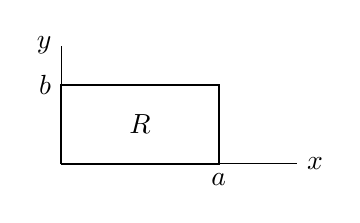
\begin{tikzpicture}
\draw(0,0)--++(3,0)node[right]{$x$};
\draw(0,0)--++(0,1.5)node[left]{$y$};
\draw[thick](0,0)--++(2,0)node[below]{$a$}--++(0,1)--++(-2,0)node[left]{$b$}--++(0,-1);
\draw(1,0.5)node{$R$};
\end{tikzpicture}
\caption{مستطیل جھلی}
\label{شکل_جزوی_مستطیل_جھلی}
\end{figure}
\موٹا{پہلا قدم۔} \quad علیحدگی متغیرات کی ترکیب استعمال کرتے ہوئے ہم پہلے مساوات \حوالہ{مساوات_جزوی_مستطیل_جھلی_الف} کا ایسا حل تلاش کرتے ہیں جو سرحدی شرط مساوات \حوالہ{مساوات_جزوی_مستطیل_جھلی_ب} کو مطمئن کرتا ہو۔یوں
\begin{align}\label{مساوات_جزوی_مستطیل_جھلی_ٹ}
u(x,y,t)=F(x,y)G(t)
\end{align}
کو مساوات \حوالہ{مساوات_جزوی_مستطیل_جھلی_الف} میں پر کرتے ہیں
\begin{align*}
F\ddot{G}=c^2(F_{xx}G+F_{yy}G)
\end{align*}
جہاں \عددی{(')} جزوی تفرق اور \عددی{(^.)} وقت \عددی{t} کے ساتھ تفرق کو ظاہر کرتے ہیں۔دونوں اطراف کو \عددی{c^2FG} سے تقسیم کرتے ہوئے
\begin{align*}
\frac{\ddot{G}}{c^2G}=\frac{1}{F}(F_{xx}+F_{yy})
\end{align*}
ملتا ہے۔اب بایاں ہاتھ تفاعل \عددی{t} پر منحصر ہے جبکہ دایاں ہاتھ  تفاعل \عددی{t} پر منحصر نہیں ہے لہٰذا دونوں اطراف کسی مستقل \عددی{A} کے برابر ہیں۔آپ   حصہ \حوالہ{حصہ_جزوی_علیحدگی_متغیرات} کی طرح  بڑھتے ہوئے تسلی کر سکتے ہیں کہ  \عددی{A} کے صرف منفی قیمتیں استعمال کرنے سے ایسا غیر صفر حل حاصل ہو گا جو مساوات \حوالہ{مساوات_جزوی_مستطیل_جھلی_ب} کی شرط کو مطمئن کرتا ہو۔اس منفی مستقل کو \عددی{-\nu^2} سے ظاہر کرتے ہوئے 
\begin{align*}
\frac{\ddot{G}}{c^2G}=\frac{1}{F}(F_{xx}+F_{yy})=-\nu^2
\end{align*}
حاصل ہوتا ہے جس کو دو علیحدہ علیحدہ سادہ تفرقی مساوات
\begin{align}
&\ddot{G}+\lambda^2G=0\quad \quad\quad (\lambda=c\nu)\label{مساوات_جزوی_مستطیل_جھلی_ث}\\
&F_{xx}+F_{yy}+\nu^2F=0\label{مساوات_جزوی_مستطیل_جھلی_ج}
\end{align}
کی صورت میں لکھا جا سکتا ہے۔

ہم  مساوات \حوالہ{مساوات_جزوی_مستطیل_جھلی_ج} کا حل تلاش کرتے ہیں جو جھلی کی سرحد پر صفر کے برابر ہو گا۔ہم علیحدگی متغیرات کی ترکیب دوبارہ لاگو کرتے ہوئے
\begin{align}
F(x,y)=H(x)Q(y)
\end{align}
لیتے ہیں جو کو مساوات \حوالہ{مساوات_جزوی_مستطیل_جھلی_ج} میں پر کرنے سے 
\begin{align*}
\frac{\dif^{\,2} H}{\dif x^2}Q=-\big(H\frac{\dif^{\,2} Q}{\dif y^2}+\nu^2HQ\big)
\end{align*}
حاصل ہوتا ہے جس کے دونوں اطراف کو \عددی{HQ} سے تقسیم کرتے ہوئے
\begin{align*}
\frac{1}{H}\frac{\dif^{\,2}H}{\dif x^2}=-\frac{1}{Q}\big(\frac{\dif^{\,2}Q}{\dif y^2}+\nu^2Q\big)
\end{align*}
ملتا ہے جہاں بائیں ہاتھ تفاعل صرف \عددی{x} پر منحصر ہے جبکہ دایاں ہاتھ تفاعل صرف \عددی{y} پر منحصر ہے۔یوں دونوں ہاتھ کسی مستقل کے برابر ہوں گے۔یہاں بھی صرف منفی قیمت کا مستقل مثلاً \عددی{-k^2} غیر صفر حل دیتے ہیں۔یوں
\begin{align*}
\frac{1}{H}\frac{\dif^{\,2}H}{\dif x^2}=-\frac{1}{Q}\big(\frac{\dif^{\,2}Q}{\dif y^2}+\nu^2Q\big)=-k^2
\end{align*}
لکھا جا سکتا ہے جس سے دو عدد سادہ تفرقی مساوات 
\begin{align}
\frac{\dif^{\,2}H}{\dif x^2}+k^2H&=0\label{مساوات_جزوی_جھلی_ایکس}\\
\frac{\dif^{\,2}Q}{\dif y^2}+p^2Q&=0\quad \quad \quad (p^2=\nu^2-k^2)\label{مساوات_جزوی_جھلی_وائے}
\end{align}
حاصل ہوتے ہیں۔

\موٹا{دوسرا قدم۔}\quad مساوات \حوالہ{مساوات_جزوی_جھلی_ایکس} اور مساوات \حوالہ{مساوات_جزوی_جھلی_وائے} کے حل عمومی
\begin{align*}
H(x)=A\cos kx+B\sin kx \quad \text{اور}\quad Q(y)=C\cos py+D\sin py
\end{align*}
ہیں جہاں \عددی{A}، \عددی{B}، \عددی{C} اور \عددی{D} مستقل ہیں۔یوں مساوات \حوالہ{مساوات_جزوی_مستطیل_جھلی_ٹ} اور مساوات \حوالہ{مساوات_جزوی_مستطیل_جھلی_ب} سے ظاہر ہے کہ جھلی کی سرحد پر \عددی{F=HQ} صفر ہو گا۔جیسا آپ شکل \حوالہ{شکل_جزوی_مستطیل_جھلی} سے دیکھ سکتے ہیں، جھلی کی سرحد \عددی{x=0}، \عددی{x=a}، \عددی{y=0} اور \عددی{y=b} ہے۔یوں درج ذیل شرائط لکھے جا سکتے ہیں۔
\begin{align*}
H(0)=0,\quad H(a)=0,\quad Q(0)=0,\quad Q(b)=0
\end{align*}
اس طرح \عددی{H(0)=A=0} ہو گا جبکہ
\begin{align*}
H(a)=B\sin ka=0
\end{align*}
میں \عددی{B=0} لینے سے (غیر دلچسپ حل) \عددی{H\equiv 0} یعنی \عددی{F \equiv 0} ملتا ہے لہٰذا ہم \عددی{B\ne 0} فرض کرتے ہیں۔یوں \عددی{\sin ka=0} ہو گا جس سے \عددی{ka=m\pi} یعنی
\begin{align}
k=\frac{m\pi}{a}\quad \quad \quad (\text{\RL{عدد صحیح $m$}})
\end{align}
حاصل ہوتا ہے۔ بالکل اسی طرح \عددی{C=0} جبکہ \عددی{D \ne 0} سے \عددی{p=\tfrac{n\pi}{b}} حاصل ہوتا ہے جہاں \عددی{n} عدد صحیح ہے۔یوں درج ذیل حل ملتے ہیں۔
\begin{align*}
H_m(x)=\sin \frac{m\pi x}{a}\quad \text{اور}\quad Q_n(y)=\sin\frac{n\pi y}{b}
\quad \quad  \substack{m=1,2,\cdots\\n=1,2,\cdots}
\end{align*}
(ارتعاش پذیر تار کی طرح یہاں بھی \عددی{m,n=-1,-2,\cdots} لینے کی ضرورت نہیں ہے چونکہ ایسا کرنے سے یہی حل ضرب \عددی{-1} دوبارہ حاصل ہوتے ہیں۔) یوں  \عددی{B=1} اور \عددی{D=1} چنتے ہوئے مساوات \حوالہ{مساوات_جزوی_مستطیل_جھلی_ج} کے حل درج ذیل ہوں گے
\begin{align}\label{مساوات_جزوی_مستطیل_مستقل_الف}
F_{mn}(x,y)=H_m(x)Q_n(y)=\sin \frac{m\pi x}{a}\sin\frac{n\pi y}{b} \quad \quad \substack{m=1,2,\cdots\\n=1,2,\cdots}
\end{align}
جو جھلی کی سرحد پر صفر کے برابر ہیں۔

چونکہ مساوات \حوالہ{مساوات_جزوی_جھلی_وائے} میں \عددی{p^2=\nu^2-k^2} ہے اور مساوات \حوالہ{مساوات_جزوی_مستطیل_جھلی_ث} میں \عددی{\lambda=c\nu} ہے  لہٰذا
\begin{align*}
\lambda=c\sqrt{k^2+p^2}
\end{align*}
ہو گا۔یوں \عددی{k=\tfrac{m\pi}{a}} اور \عددی{p=\tfrac{n\pi}{b}} کا مطابقتی \عددی{\lambda} مساوات \حوالہ{مساوات_جزوی_مستطیل_جھلی_ث} میں
\begin{align}\label{مساوات_جزوی_مستطیل_مستقل_ب}
\lambda=\lambda_{mn}=c\pi\sqrt{\frac{m^2}{a^2}+\frac{n^2}{b^2}}\quad \quad \substack{m=1,2,\cdots\\n=1,2,\cdots}
\end{align}
ہو گا اور مساوات \حوالہ{مساوات_جزوی_مستطیل_جھلی_ث} کا مطابقتی  عمومی حل درج ذیل ہو گا۔
\begin{align*}
G_{mn}(t)=B_{mn}\cos \lambda_{mn}t+B^*_{mn}\sin \lambda_{mn}t
\end{align*}
یوں مساوات \حوالہ{مساوات_جزوی_مستطیل_جھلی_ث} کے غیر صفر  حل \عددی{u_{mn}(x,y,t)=F_{mn}(x,y)G_{mn}(t)} درج ذیل ہوں گے
\begin{align}\label{مساوات_جزوی_مستطیل_مستقل_پ}
u_{mn}(x,y,t)=(B_{mn}\cos \lambda_{mn}t+B^*_{mn}\sin \lambda_{mn}t)\sin \frac{m\pi x}{a}\sin \frac{n\pi y}{b}
\end{align}
 جن میں \عددی{\lambda_{mn}} مساوات \حوالہ{مساوات_جزوی_مستطیل_مستقل_ب} دے گی۔ تفاعل \عددی{u_{mn}} کو ارتعاش پذیر جھلی کے \اصطلاح{آئگنی تفاعل}\فرہنگ{آئگنی!تفاعل}\حاشیہب{eigenfunctions}\فرہنگ{eigenfunctions} یا \اصطلاح{امتیازی تفاعل}\فرہنگ{امتیازی!تفاعل}\حاشیہب{characteristic functions}\فرہنگ{characteristic!functions} کہتے ہیں جبکہ \عددی{\lambda_{mn}} کو ارتعاش پذیر جھلی کے \اصطلاح{آئگنی اقدار}\فرہنگ{آئگنی!اقدار}\حاشیہب{eigenvalues}\فرہنگ{eigenvalues} یا \اصطلاح{امتیازی اقدار}\فرہنگ{امتیازی!اقدار}\حاشیہب{characteristic values}\فرہنگ{characteristic!values} کہتے ہیں۔تفاعل \عددی{u_{mn}} کی تعدد \عددی{\tfrac{\lambda_{mn}}{2\pi}} ہو گی۔

\عددی{a} اور \عددی{b} کی مختلف قیمتیں ایک ہی  امتیازی قدر دیتے ہوئے کئی مختلف  تفاعل \عددی{F_{mn}} دے سکتی ہیں۔اس کا مطلب ہے کہ جھلی میں ایک ہی تعدد کے  کئی مختلف انداز کے ارتعاش ممکن ہیں جن کی  \اصطلاح{صفر ہٹاو لکیریں}\فرہنگ{صفر ہٹاو!لکیر}\حاشیہب{nodal lines}\فرہنگ{nodal!lines} مختلف ہوں گی۔ ارتعاش پذیر جھلی پر وہ لکیریں جو حرکت نہیں کرتی ہیں صفر ہٹاو لکیریں کہلاتی ہیں۔آئیں اس کی وضاحت ایک مثال کی مدد سے سمجھیں۔

%=================
\ابتدا{مثال}\شناخت{مثال_جزوی_مکعب_جھلی}\quad مکعب جھلی\\
ایک مکعب جھلی کا \عددی{a=1}، \عددی{b=1} ہے۔مساوات \حوالہ{مساوات_جزوی_مستطیل_مستقل_ب} سے 
\begin{align}\label{مساوات_جزوی_مثال_مکعب_جھلی_الف}
\lambda_{mn}=c\pi\sqrt{m^2+n^2}
\end{align}
لہٰذا 
\begin{align*}
\lambda_{mn}=\lambda{nm}
\end{align*}
ہو گا لیکن \عددی{m \ne n} کے لئے مطابقتی  تفاعل
\begin{align*}
F_{mn}=\sin m\pi x\,\sin n\pi y \quad \text{اور} \quad F_{nm}=\sin n\pi x\,\sin m\pi y
\end{align*}
ہیں جو ایک جیسے نہیں ہیں۔مثلاً \عددی{\lambda_{12}=\lambda_{21}=c\pi\sqrt{5}} کے مطابقتی تفاعل
\begin{align*}
F_{12}=\sin \pi x\,\sin 2\pi y\quad \text{اور}\quad F_{21}=\sin 2\pi x\,\sin \pi y
\end{align*}
ہوں گے۔یوں مطابقتی حل
\begin{align*}
u_{12}&=(B_{12}\cos c\pi\sqrt{5}t+B^*_{12}\sin c\pi\sqrt{5}t)F_{12}\\
u_{21}&=(B_{21}\cos c\pi\sqrt{5}t+B^*_{21}\sin c\pi\sqrt{5}t)F_{21}\\
\end{align*}
کی صفر ہٹاو لکیریں  بالترتیب \عددی{y=\tfrac{1}{2}} اور \عددی{x=\tfrac{1}{2}} ہوں گی (شکل \حوالہ{شکل_مثال_جزوی_مکعب_جھلی}-الف)۔اگر \عددی{B_{12}=1} اور \عددی{B^*_{12}=B^*_{21}=0} ہوں تب
\begin{align}\label{مساوات_جزوی_ایک_بی_کے_حل}
u_{12}+u_{21}=\cos c\pi\sqrt{5}t\,(F_{12}+B_{21}F_{21})
\end{align}
ہو گا جو ایک اور انداز ارتعاش ہے جس کی امتیازی قدر \عددی{c\pi\sqrt{5}} ہے۔اس تفاعل کی صفر ہٹاو لکیریں درج ذیل مساوات کے حل ہوں گی۔
\begin{align*}
F_{12}+B_{21}F_{21}=\sin \pi x\,\sin 2\pi y+B_{21}\sin 2\pi x\,\sin \pi y=0
\end{align*}
اب \عددی{\sin 2\alpha=2\sin \alpha \cos \alpha} استعمال کرتے ہوئے درج بالا کو 
\begin{align}
\sin \pi x\sin \pi y(\cos \pi y+B_{21}\cos \pi x)=0
\end{align}
لکھا جا سکتا ہے جس کا حل \عددی{B_{21}} پر منحصر ہو گا (شکل \حوالہ{شکل_مثال_جزوی_مکعب_جھلی}-ب)۔

مساوات \حوالہ{مساوات_جزوی_مثال_مکعب_جھلی_الف} سے ہم دیکھتے ہیں کہ \عددی{\lambda_{mn}} کے دو مزید مطابقتی تفاعل ممکن ہیں۔مثلاً چار تفاعل \عددی{F_{18}}، \عددی{F_{81}}، \عددی{F_{47}} اور \عددی{F_{74}} کی \عددی{\lambda_{18}=\lambda_{81}=\lambda_{47}=\lambda_{74}=c\pi\sqrt{65}} ہے چونکہ؛
\begin{align*}
1^1+8^2=4^2+7^2=65
\end{align*}
ایسا اس لئے ممکن ہے  کہ  \عددی{65} کو  دو اعداد صحیح کے مربع کا مجموعہ مختلف طریقوں سے لکھنا ممکن ہے۔گاوس کے ایک مسئلہ کے تحت ایسا ہر اس صورت ہو گا جہاں دو اعداد کے مربع کا مجموعہ کے اجزاء مفرد میں کم از کم دو مختلف \عددی{4n+1} صورت کے ہوں، جہاں \عددی{n} مثبت عدد صحیح ہے۔یہاں دو اعداد کے مربع کے مجموعہ \عددی{65} کو 
\begin{align*}
65=5\cdot13=(4+1)(12+1)
\end{align*}
لکھنا ممکن ہے۔
\begin{figure}
\centering
\begin{subfigure}{0.5\textwidth}
\centering
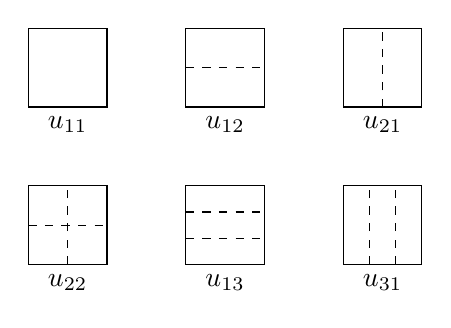
\begin{tikzpicture}
\pgfmathsetmacro{\w}{2}
\pgfmathsetmacro{\ll}{\w/2}
%
\draw(0,0) rectangle ++(1,1);
\draw(0.5,0)node[below]{$u_{11}$};
%
\draw(1*\w,0) rectangle ++(1,1);
\draw(1*\w+0.5,0)node[below]{$u_{12}$};
\draw[dashed](1*\w,0.5)--++(1,0);
%
\draw(2*\w,0) rectangle ++(1,1);
\draw(2*\w+0.5,0)node[below]{$u_{21}$};
\draw[dashed](2*\w+0.5,0)--++(0,1);
%
\draw(0*\w,-\w) rectangle ++(1,1);
\draw(0*\w+0.5,-\w)node[below]{$u_{22}$};
\draw[dashed](0*\w+0.5,-\w)--++(0,1);
\draw[dashed](0*\w,-\w+0.5)--++(1,0);
%
\draw(1*\w,-\w) rectangle ++(1,1);
\draw(1*\w+0.5,-\w)node[below]{$u_{13}$};
\draw[dashed](1*\w,-\w+1/3*\ll)--++(1,0);
\draw[dashed](1*\w,-\w+2/3*\ll)--++(1,0);
%
\draw(2*\w,-\w) rectangle ++(1,1);
\draw(2*\w+0.5,-\w)node[below]{$u_{31}$};
\draw[dashed](2*\w+1/3*\ll,-\w)--++(0,1);
\draw[dashed](2*\w+2/3*\ll,-\w)--++(0,1);
\end{tikzpicture}
\caption*{(الف) مکعب جھلی کے حل $u_{11},u_{12},u_{21},u_{22},u_{13}, u_{31}$ کی صفر ہٹاو لکیریں۔}
\end{subfigure}%
\begin{subfigure}{0.5\textwidth}
\centering
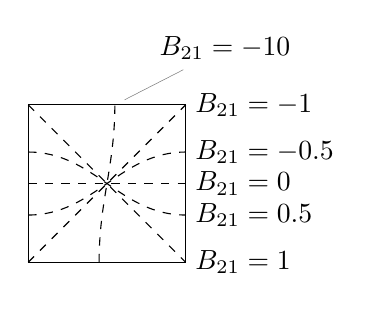
\begin{tikzpicture}
\pgfmathsetmacro{\len}{2}
\draw(0,0) rectangle ++(\len,\len);
\draw[dashed] (0,0.5*\len)--++(1*\len,0)node[right]{$B_{21}=0$};
\draw[dashed](0.45*\len,0) to [out=90,in=-90](0.55*\len,1*\len)coordinate(kA);
\draw(kA)node[pin=45:{$B_{21}=-10$}]{};
\draw[dashed](0,0)--++(1*\len,1*\len)node[right]{$B_{21}=-1$};
\draw[dashed](0,1*\len)--++(1*\len,-1*\len)node[right]{$B_{21}=1$};
\draw[dashed](0,0.3*\len) to [out=0,in=180] ++(1*\len,0.4*\len)node[right]{$B_{21}=-0.5$};
\draw[dashed](0,0.7*\len) to [out=0,in=180] ++(1*\len,-0.4*\len)node[right]{$B_{21}=0.5$};
\end{tikzpicture}
\caption*{(ب) ایک ہی $B_{21}$ کے لئے مساوات \حوالہ{مساوات_جزوی_ایک_بی_کے_حل} میں دیے گئے حل}
\end{subfigure}%
\caption{صفر ہٹاو لکیریں (مثال \حوالہ{مثال_جزوی_مکعب_جھلی})}
\label{شکل_مثال_جزوی_مکعب_جھلی}
\end{figure}
\انتہا{مثال}
%============================

\موٹا{تیسرا قدم۔}\quad ایسا حل جو ابتدائی شرائط مساوات \حوالہ{مساوات_جزوی_مستطیل_جھلی_پ} اور مساوات \حوالہ{مساوات_جزوی_مستطیل_جھلی_ت} کو مطمئن کرتا ہو حاصل کرنے کی خاطر ہم  حصہ \حوالہ{حصہ_جزوی_علیحدگی_متغیرات} کی طرح بڑھتے ہیں۔ہم دوہرا تسلسل\حاشیہد{ہم حل کی یکتائی اور ارتکاز پر غور نہیں کریں گے۔}
\begin{gather}
\begin{aligned}\label{مساوات_جزوی_مکمل_حل_مستطیل_جھلی}
u(x,y,t)&=\sum_{m=1}^{\infty}\sum_{n=1}^{\infty} u_{mn}(x,y,t)\\
&=\sum_{m=1}^{\infty}\sum_{n=1}^{\infty}(B_{mn}\cos \lambda_{mn}t+B^*_{mn}\sin \lambda_{mn}t)\sin\frac{m\pi x}{a}\sin \frac{n\pi y}{b}
\end{aligned}
\end{gather}
کو لیتے ہیں جو مساوات \حوالہ{مساوات_جزوی_مستطیل_جھلی_پ} کے ساتھ درج ذیل  \اصطلاح{دوہرا فوریئر تسلسل}\فرہنگ{فوریئر!دوہرا تسلسل}\حاشیہب{double Fourier series}\فرہنگ{Fourier!double series} دیتی ہے۔
\begin{align}\label{مساوات_جزوی_دوہرا_فوریئر_تسلسل_الف}
u(x,y,0)=\sum_{m=1}^{\infty}\sum_{n=1}^{\infty}B_{mn}\sin\frac{m\pi x}{a}\sin \frac{n\pi y}{b}=f(x,y)
\end{align}
مستطیل \عددی{R} (شکل \حوالہ{شکل_جزوی_مستطیل_جھلی}) میں \عددی{f}، \عددی{\tfrac{\partial f}{\partial x}}، \عددی{\tfrac{\partial f}{\partial y}} اور \عددی{\tfrac{\partial^{\,2}f}{\partial x\partial y}} استمراری ہونے کی صورت میں \عددی{f(x,y)} کو اس دوہرا فوریئر تسلسل کی صورت میں لکھنا ممکن ہو گا۔اس دوہرا فوریئر تسلسل کے عددی سر حاصل کرتے ہیں۔ہم درج ذیل لے کر
\begin{align}\label{مساوات_جزوی_دوہرا_فوریئر_تسلسل_ب}
K_m(y)=\sum_{n=1}^{\infty}B_{mn}\sin \frac{n\pi y}{b}
\end{align}
مساوات \حوالہ{مساوات_جزوی_دوہرا_فوریئر_تسلسل_الف} کو
\begin{align}\label{مساوات_جزوی_دوہرا_فوریئر_تسلسل_پ}
f(x,y)=\sum_{n=1}^{\infty}K_m(y)\sin \frac{m\pi x}{a}
\end{align}
لکھ سکتے ہیں جو مقررہ \عددی{y} کی صورت میں \عددی{f(x,y)} کی  فوریئر سائن تسلسل ہے جس کا متغیرہ \عددی{x} ہو گا جس کے عددی سر صفحہ \حوالہصفحہ{مساوات_فوریئر_نصف_حلقہ_توسیع_طاق_عددی_سر} پر مساوات \حوالہ{مساوات_فوریئر_نصف_حلقہ_توسیع_طاق_عددی_سر} کے تحت
\begin{align}\label{مساوات_جزوی_دوہرا_فوریئر_تسلسل_ت}
K_m(y)=\frac{2}{a}\int_0^a f(x,y)\sin\frac{m\pi x}{a}\dif x
\end{align}
ہوں گے۔مزید مساوات \حوالہ{مساوات_جزوی_دوہرا_فوریئر_تسلسل_ب} تفاعل \عددی{K_m(y)} کی فوریئر سائن تسلسل ہے لہٰذا اس کے عددی سر صفحہ \حوالہصفحہ{مساوات_فوریئر_نصف_حلقہ_توسیع_طاق_عددی_سر} پر مساوات \حوالہ{مساوات_فوریئر_نصف_حلقہ_توسیع_طاق_عددی_سر} کے تحت
\begin{align}\label{مساوات_جزوی_دوہرا_فوریئر_تسلسل_ٹ}
B_{mn}=\frac{2}{b}\int_0^b K_m(y)\sin \frac{n\pi y}{b}\dif y
\end{align}
ہوں گے۔مساوات \حوالہ{مساوات_جزوی_دوہرا_فوریئر_تسلسل_ٹ} اور مساوات \حوالہ{مساوات_جزوی_دوہرا_فوریئر_تسلسل_ت} کو ملا کر درج ذیل \اصطلاح{عمومی یولر کلیہ}\فرہنگ{یولر!عمومی کلیہ}\حاشیہب{generalized Euler formula}\فرہنگ{Euler!generalized formula} حاصل ہوتا ہے
\begin{align}\label{مساوات_جزوی_دوہرا_فوریئر_تسلسل_ث}
B_{mn}=\frac{4}{ab}\int_0^b\int_0^a f(x,y)\sin\frac{m\pi x}{a}\,\sin \frac{n\pi y}{b} \dif x\,\dif y\quad \quad \substack{m=1,2,\cdots\\n=1,2,\cdots}
\end{align}
جو دوہرا تسلسل (مساوات \حوالہ{مساوات_جزوی_دوہرا_فوریئر_تسلسل_الف}) میں تفاعل \عددی{f(x,y)} کے عددی سر \عددی{B_{mn}} دیتی ہے۔

یوں مساوات \حوالہ{مساوات_جزوی_مکمل_حل_مستطیل_جھلی} میں \عددی{B_{mn}} تفاعل \عددی{f(x,y)} سے حاصل ہوتے ہیں۔ \عددی{B^*_{mn}} حاصل کرنے کی خاطر ہم مساوات \حوالہ{مساوات_جزوی_مکمل_حل_مستطیل_جھلی} کا \عددی{t} کے ساتھ جزوی تفرق لے کر ابتدائی شرط مساوات \حوالہ{مساوات_جزوی_مستطیل_جھلی_ت} استعمال کرتے ہوئے  
\begin{align*}
\left.\frac{\partial u}{\partial t}\right|_{t=0}=\sum_{m=1}^{\infty}\sum_{n=1}^{\infty} B^*_{mn}\lambda_{mn}\sin\frac{m\pi x}{a}\,\sin\frac{n\pi y}{b}=g(x,y)
\end{align*}
حاصل کرتے ہیں۔ مستطیل \عددی{R} (شکل \حوالہ{شکل_جزوی_مستطیل_جھلی}) میں \عددی{g}، \عددی{\tfrac{\partial g}{\partial x}}، \عددی{\tfrac{\partial g}{\partial y}} اور \عددی{\tfrac{\partial^{\,2}u}{\partial x\partial y}}  استمراری ہونے کی صورت میں \عددی{g(x,y)} کو اس دوہرا فوریئر تسلسل کی صورت میں لکھا جا سکتا ہے۔یوں پہلی کی طرح بڑھتے ہوئے درج ذیل حاصل ہو گا۔
\begin{align}\label{مساوات_جزوی_دوہرا_فوریئر_تسلسل_ج}
B^*_{mn}=\frac{4}{ab\lambda_{mn}}\int_0^b\int_0^a g(x,y) \sin\frac{m\pi x}{a}\,\sin \frac{n\pi y}{b}\dif x\dif y\quad \quad \substack{m=1,2,\cdots\\n=1,2,\cdots}
\end{align}
یوں مساوات \حوالہ{مساوات_جزوی_دوہرا_فوریئر_تسلسل_ث} اور مساوات \حوالہ{مساوات_جزوی_دوہرا_فوریئر_تسلسل_ج} سے حاصل \عددی{B_{mn}} اور \عددی{B^*_{mn}}   مساوات \حوالہ{مساوات_جزوی_مکمل_حل_مستطیل_جھلی} میں پر کرتے ہوئے حاصل حل ابتدائی شرائط کو مطمئن کرے گا۔

%===================
\حصہء{سوالات}

%===============
\ابتدا{سوال}\quad
جھلی میں تناو بڑھانے سے مساوات \حوالہ{مساوات_جزوی_مستطیل_مستقل_پ} میں دی گئی حل کی تعدد پر کیا اثر ہو گا؟\\
جواب:\quad چونکہ \عددی{c} بڑھتا ہے لہٰذا تعدد بھی بڑھے گی۔
\انتہا{سوال}
%=====================
\ابتدا{سوال}\quad
مساوات \حوالہ{مساوات_جزوی_مستطیل_مستقل_پ} کی صفر ہٹاو لکیریں \عددی{a=b=1} لے کر  \عددی{m=1,2,3,4} اور \عددی{n=1,2,3,4} کے لئے کھینچیں۔ 
\انتہا{سوال}
%===================
\ابتدا{سوال}\quad
مساوات \حوالہ{مساوات_جزوی_مستطیل_مستقل_پ} کی صفر ہٹاو لکیریں \عددی{a=2} اور \عددی{b=1} لے کر  \عددی{m=1,2,3,4} اور \عددی{n=1,2,3,4} کے لئے کھینچیں۔ 
\انتہا{سوال}
%===================
\ابتدا{سوال}\quad
اکائی لمبائی کے اطراف والی مکعب جھلی کے مزید ایسے امتیازی اقدار حاصل کریں جن کے مطابقتی امتیازی تفاعل کی تعدد چار عدد ہو۔
\انتہا{سوال}
%==============
\ابتدا{سوال}\quad
مستطیل جھلی جس کے اطراف \عددی{a=2} اور \عددی{b=1} ہیں کے ایسے امتیازی اقدار حاصل کریں جن کے مطابقتی امتیازی تفاعل کی تعدد دو یا دو سے زیادہ ہو۔\\
جواب:\quad
$c\pi\sqrt{260}, \quad (F_{4,16},F_{16,14}),\cdots $
\انتہا{سوال}
%==============
\ابتدا{سوال}\شناخت{سوال_جزوی_کمتر_تعدد_شکل_جھلی_الف}\quad
تصدیق کرین کہ یکساں \عددی{c} والی تمام ممکنہ مستطیل جھلی جن کا رقبہ \عددی{A} ہو میں مکعب جھلی  کی \عددی{u_{11}} (مساوات \حوالہ{مساوات_جزوی_مستطیل_مستقل_پ}) کی تعدد کم تر ہو گی۔
\انتہا{سوال}
%====================
\ابتدا{سوال}\شناخت{سوال_جزوی_کمتر_تعدد_شکل_جھلی_ب}\quad
مقررہ \عددی{m}، \عددی{n} اور \عددی{A} کے لئے  سوال \حوالہ{سوال_جزوی_کمتر_تعدد_شکل_جھلی_الف} کی طرح کم تر تعدد کی شرط اخذ کریں۔\\
جواب:\quad مساوات \حوالہ{مساوات_جزوی_مستطیل_مستقل_ب} میں \عددی{a=\tfrac{A}{b}} پر کرتے ہوئے حاصل \عددی{\lambda} کا \عددی{a} کے ساتھ تفرق، صفر کے برابر کرتے ہوئے
\begin{align*}
\lambda^2=c^2\pi^2\big(\frac{m^2}{a^2}+\frac{n^2a^2}{A^2}\big),\implies 2\lambda \frac{\dif \lambda}{\dif a}=c^2\pi^2\big(-\frac{2m^2}{a^3}+\frac{2n^2a}{A^2}\big)=0
\end{align*}
 کمتر \عددی{\lambda} کی شرط 
$\tfrac{m}{a}=\tfrac{n}{b}$
حاصل کرتے ہیں۔
\انتہا{سوال}
%====================

سوال \حوالہ{سوال_جزوی_دوہرا_فوریئر_تسلسل_الف} تا سوال \حوالہ{سوال_جزوی_دوہرا_فوریئر_تسلسل_ب} میں تفاعل \عددی{f(x,y)\quad (0<x<a, 0<y<b)} کا مساوات \حوالہ{مساوات_جزوی_دوہرا_فوریئر_تسلسل_الف} کی طرز کا دوہرا فوریئر تسلسل حاصل کریں۔

%============
\ابتدا{سوال}\شناخت{سوال_جزوی_دوہرا_فوریئر_تسلسل_الف}\quad
$f=1$\\
جواب:\quad
$B_{mn}=\tfrac{16}{mn\pi^2}, \quad m,n=1,3,5,\cdots$
\انتہا{سوال}
%===================
\ابتدا{سوال}\quad
$f=x+y$\\
جواب:\quad
$B_{mn}=\tfrac{4}{mn\pi^2}[a(-1)^{m+n}-a(-1)^m+b(-1)^{m+n}-b(-1)^n]$
\انتہا{سوال}
%===================
\ابتدا{سوال}\quad
$f=xy$\\
جواب:\quad
$B_{mn}=\tfrac{4ab(-1)^{m+n}}{mn\pi^2}$
\انتہا{سوال}
%===================
\ابتدا{سوال}\quad
$f=xy(a-x)(b-y)$\\
جواب:\quad
$B_{mn}=\tfrac{64a^2b^2}{m^3n^3\pi^6},\quad m,n=1,3,5,\cdots$
\انتہا{سوال}
%===================
\ابتدا{سوال}\شناخت{سوال_جزوی_دوہرا_فوریئر_تسلسل_ب}\quad
$f=xy(a^2-x^2)(b^2-y^2)$\\
جواب:\quad
$B_{mn}=\tfrac{144a^3b^3(-1)^{m+n}}{m^3n^3\pi^6}$
\انتہا{سوال}
%===================
\ابتدا{سوال}\quad
ثابت کریں کہ فی اکائی رقبہ بیرونی قوت \عددی{P(x,y,t)} کی صورت میں \عددی{xy} مستوی میں جھلی کی ارتعاش درج ذیل مساوات دیتی ہے جہاں فی اکائی رقبہ جھلی کی کمیت \عددی{\rho} ہے۔بیرونی قوت جھلی کی عمودی عمل کرتی ہے۔
\begin{align*}
u_{tt}=c^2\nabla^{\,2}u+\frac{P}{\rho}
\end{align*}
\انتہا{سوال}
%==================
سوال \حوالہ{سوال_جزوی_جھلی_انحراف_الف} تا سوال \حوالہ{سوال_جزوی_جھلی_انحراف_ب} میں ابتدائی رفتار صفر  جبکہ ابتدائی انحراف \عددی{f(x,y)} ہے۔جھلی کی انحراف \عددی{u(x,y,t)} دریافت کریں جہاں \عددی{c=1} اور \عددی{a=b=1} ہیں۔

%=================
\ابتدا{سوال}\شناخت{سوال_جزوی_جھلی_انحراف_الف}\quad
$f=0.1xy(1-x)(1-y)$\\
جواب:\quad
\begin{align*}
u(x,y,t)=\frac{6.4}{\pi^6}\sum_{\substack{m=1\\\text{\RL{طاق $m$}}}}^{\infty}\sum_{\substack{n=1\\\text{\RL{طاق $n$}}}}^{\infty} \tfrac{1}{m^3n^3}\cos (\pi t\sqrt{m^2+n^2})\,\sin m\pi x\,\sin n\pi y
\end{align*}
\انتہا{سوال}
%======================
\ابتدا{سوال}\quad
$f=kx(1-x^2)(1-y^2)$\\
جواب:\quad
\begin{align*}
\frac{24k}{\pi^6}\sum_{m=1}^{\infty}\sum_{n=1}^{\infty} \tfrac{(-1)^m}{m^3n^3}[2(-1)^n-(n^2\pi^2+1)]\cos (\pi t\sqrt{m^2+n^2})\,\sin m\pi x\,\sin n\pi y
\end{align*}
\انتہا{سوال}
%======================
\ابتدا{سوال}\quad
$f=k\sin \pi x\,\sin 2\pi y$\\
جواب:\quad
$u(x,y,t)=k\cos \pi \sqrt{5}t\,\sin \pi x\,\sin 2\pi y$
\انتہا{سوال}
%=================
\ابتدا{سوال}\شناخت{سوال_جزوی_جھلی_انحراف_ب}\quad
$f=k\sin^2 \pi x\,\sin^2\pi y$\\
جواب:\quad
$B_{2n}=B_{m2}=0,B_{11}=\tfrac{64k}{9\pi^2},B_{13}=-\tfrac{64k}{45\pi^2}, B_{31}=-\tfrac{64k}{45\pi^2},B_{33}=\tfrac{64k}{225\pi^2}\cdots $
\انتہا{سوال}
%=================
\ابتدا{سوال}\شناخت{سوال_جزوی_حراری_مساوات_چادر}\quad
باریک مکعب چادر کے اطراف صفر درجہ حرارت پر رکھے گئے ہیں جبکہ اس کی دونوں سطحیں حاجز شدہ ہیں۔چادر کی ایک طرف کی لمبائی \عددی{\pi} ہے۔ ابتدائی درجہ حرارت \عددی{u(x,y,0)=f(x,y)} ہے۔دو ابعادی حراری مساوات \عددی{u_t=c^2\nabla^{\,2}u} پر علیحدگی متغیرات کی ترکیب لاگو کرتے ہوئے درج ذیل حل حاصل کریں
\begin{align*}
u(x,y,t)=\sum_{m=1}^{\infty}\sum_{n=1}^{\infty} B_{mn}\sin mx \,\sin ny\,e^{-c^2(m^2+n^2)t}
\end{align*}
جہاں \عددی{B_{mn}} درج ذیل ہے۔
\begin{align*}
B_{mn}=\frac{4}{\pi^2}\int_0^{\pi}\int_0^{\infty} f(x,y)\,\sin mx\,\sin ny\,\dif x\,\dif y
\end{align*}
 
\انتہا{سوال}
%====================
\ابتدا{سوال}\quad
\عددی{f(x,y)=xy(\pi-x)(\pi-y)} کی صورت میں سوال \حوالہ{سوال_جزوی_حراری_مساوات_چادر} میں دیے گئے چادر کا حل تلاش کریں۔\\
جواب:\quad
\begin{align*}
u(x,y,t)=\sum_{m=1}^{\infty}\sum_{n=1}^{\infty} \frac{64}{m^3n^3\pi^2}\sin mx \,\sin ny\,e^{-c^2(m^2+n^2)t}
\end{align*}
\انتہا{سوال}
%======================

\حصہ{قطبی محدد میں لاپلاسی}\شناخت{حصہ_جزوی_قطبی_محدد_لاپلاسی}
سرحدی شرائط  کی جزوی تفرقی مساوات کا حل تلاش کرتے ہوئے  عموماً ایسا محدد استعمال کیا جاتا ہے جس کے لحاظ سے سرحد کی روپ سادہ ہو۔اگلے حصے میں دائری جھلی پر غور کیا جائے گا جس کو حل کرنے کے لئے \اصطلاح{قطبی محدد}\فرہنگ{قطبی محدد}\فرہنگ{محدد!قطبی}\حاشیہب{polar coordinates}\فرہنگ{polar coordinates}\فرہنگ{coordinates!polar} سود مند ثابت ہو گا جس کے متغیرات \عددی{r} اور \عددی{\theta} کی تعریف درج ذیل ہیں۔
\begin{align*}
x=r\cos \theta, \quad y&=r\sin \theta
\end{align*}
قطبی محدد میں جھلی کی  دائری سرحد کی مساوات 
$\text{مستقل}=r$
 ہو گی۔ 

\عددی{r} اور \عددی{\theta} استعمال کرتے ہوئے مساوات موج کی لاپلاسی
\begin{align*}
\nabla^{\,2}u=\frac{\partial^{\,2}u}{\partial x^2}+\frac{\partial^{\,2}u}{\partial y^2}
\end{align*}
کا اظہار ان محدد میں کرنا ہو گا لہٰذا آپ سے التماس ہے کہ درج ذیل کو غور سے پڑھیں۔

 ہم حصہ \حوالہ{حصہ_جزوی_دا_لومبیغ_حل} کی طرح زنجیری ترکیب استعمال کریں گے۔اپنی آسانی کی خاطر ہم جزوی تفرق کو زیر نوشت میں \عددی{x}، \عددی{y} یا \عددی{t} لکھ کر ظاہر کریں گے جبکہ متغیرات \عددی{r,\theta,t}  کے تفاعل \عددی{u(x,y,t)} کو اسی حرف \عددی{u} سے ظاہر کریں گے۔

صفحہ \حوالہصفحہ{مساوات_الاحصاء_زنجیری_ترکیب_کلیات}  پر مساوات \حوالہ{مساوات_الاحصاء_زنجیری_ترکیب_کلیات} کا زنجیری قاعدہ استعمال کرتے ہوئے
\begin{align*}
u_x=u_r r_x+u_{\theta}\theta_x
\end{align*}
ملتا ہے۔ایک بار دوبارہ \عددی{x} کے ساتھ تفرق لے کر درج ذیل حاصل ہو گا۔
\begin{gather}
\begin{aligned}\label{مساوات_جزوی_لاپلاسی__رکن_الف}
u_{xx}&=(u_r r_x)_x+(u_{\theta}\theta_x)_x\\
&=(u_r)_xr_x+u_rr_{xx}+(u_{\theta})_x\theta_x+u_{\theta}\theta_{xx}
\end{aligned}
\end{gather}
زنجیری قاعدہ دوبارہ استعمال کرتے ہوئے
\begin{align*}
(u_r)_x=u_{rr}r_x+u_{r\theta}\theta_x\quad \text{اور}\quad (u_{\theta})_x=u_{\theta r}r_x+u_{\theta \theta} \theta_x
\end{align*}
لکھا جا سکتا ہے۔جزوی تفرق \عددی{r_x} اور \عددی{\theta_x} حاصل کرنے کی خاطر ہمیں
\begin{align*}
r=\sqrt{x^2+y^2}\quad \text{اور}\quad \theta=\tan^{-1}\frac{y}{x}
\end{align*}
کا تفرق لینا ہو گا جس سے 
\begin{align*}
r_x=\frac{x}{\sqrt{x^2+y^2}}=\frac{x}{r}, \quad \theta_x=\frac{1}{1+\frac{y^2}{x^2}}\left(-\frac{y}{x^2}\right)=-\frac{y}{r^2}
\end{align*}
حاصل ہو گا۔ ان کا \عددی{x} تفرق لینے سے
\begin{align*}
r_{xx}=\frac{r-xr_x}{r^2}=\frac{1}{r}-\frac{x^2}{r^3}=\frac{y^2}{r^3},\quad \theta_{xx}=-y\left(-\frac{2}{r^3}\right)r_x=\frac{2xy}{r^4}
\end{align*}
ملتا ہے۔ان تمام کو مساوات \حوالہ{مساوات_جزوی_لاپلاسی__رکن_الف} میں پر کرتے ہیں۔ایک درجی اور دو درجی جزوی تفرق کو استمراری تصور کرتے ہوئے \عددی{u_{r\theta}=u_{\theta r}} لکھ کر یوں درج ذیل سادہ صورت حاصل ہو گی۔
 \begin{align}\label{مساوات_جزوی_لاپلاسی__رکن_ب}
u_{xx}=\frac{x^2}{r^2}u_{rr}-2\frac{xy}{r^3}u_{r\theta}+\frac{y^2}{r^4}u_{\theta\theta}+\frac{y^2}{r^3}u_r+2\frac{xy}{r^4}u_{\theta}
\end{align}
بالکل اسی طرح درج ذیل بھی حاصل کی جا سکتی ہے۔
\begin{align}\label{مساوات_جزوی_لاپلاسی__رکن_پ}
u_{yy}=\frac{y^2}{r^2}u_{rr}+2\frac{xy}{r^3}u_{r\theta}+\frac{x^2}{r^4}u_{\theta\theta}+\frac{x^2}{r^3}u_r-2\frac{xy}{r^4}u_{\theta}
\end{align}
مساوات \حوالہ{مساوات_جزوی_لاپلاسی__رکن_ب} اور مساوات \حوالہ{مساوات_جزوی_لاپلاسی__رکن_پ} کا مجموعہ لے کر قطبی محدد میں لاپلاسی حاصل کرتے ہیں۔
\begin{align}\label{مساوات_جزوی_لاپلاسی__رکن_ت}
\nabla^{\,2}u=\frac{\partial^{\,2}u}{\partial r^2}+\frac{1}{r}\frac{\partial u}{\partial r}+\frac{1}{r^2}\frac{\partial^{\,2}u}{\partial \theta^2}
\end{align}

%===========================
\حصہء{سوالات}
%================
\ابتدا{سوال}\quad
مساوات \حوالہ{مساوات_جزوی_لاپلاسی__رکن_ت} کو درج ذیل صورت میں لکھ کر دکھائیں۔
\begin{align*}
\nabla^{\,2}u=\frac{1}{r}\frac{\partial}{\partial r}\big(r\frac{\partial u}{\partial r}\big)+\frac{1}{r^2}\frac{\partial^{\,2}u}{\partial \theta^2}
\end{align*}
\انتہا{سوال}
%======================
\ابتدا{سوال}\quad
اگر مساوات \حوالہ{مساوات_جزوی_لاپلاسی__رکن_ت} میں لاپلاسی \عددی{\theta} سے آزاد ہو  تب \عددی{\nabla^{\,2}u=u_{rr}+\tfrac{u_r}{r}} لکھی جائے گی۔ \عددی{u} کو \عددی{\theta} سے آزاد فرض کرتے ہوئے کارتیسی محدد میں لاپلاسی سے سیدھا  یہ نتیجہ حاصل کریں۔
\انتہا{سوال}
%==================
\ابتدا{سوال}\quad
مساوات \حوالہ{مساوات_جزوی_لاپلاسی__رکن_ت} کو واپس کارتیسی محدد میں لے جائیں۔
\انتہا{سوال}
%====================
\ابتدا{سوال}\quad
اگر \عددی{x}، \عددی{y} کارتیسی محدد ہوں تب دکھائیں کہ \عددی{x^*=x\cos \alpha-y\sin \alpha} اور \عددی{y^*=x\sin \alpha+y\cos \alpha} بھی کارتیسی محدد ہیں۔ لاپلاسی کو کارتیسی محدد \عددی{x^*}، \عددی{y^*} میں حاصل کریں۔\\
جواب:\quad
$\nabla^{\,2}u=u_{x^*x^*}+u_{y^*y^*}$ 
\انتہا{سوال}
%=======================
\ابتدا{سوال}\quad
لاپلاسی \عددی{\nabla^{\,2}u} کو نئی محدد \عددی{x^*=ax+b}، \عددی{y^*=cy+d} میں لکھیں جہاں \عددی{x}، \عددی{y} کارتیسی محدد ہیں جبکہ \عددی{a}، \عددی{b}، \عددی{c} اور \عددی{d} مستقل ہیں۔\\
جواب:\quad
$\nabla^{\,2}u=a^2u_{x^*x^*}+c^2u_{y^*y^*}$
\انتہا{سوال}
%====================
\ابتدا{سوال}\quad \موٹا{\اصطلاح{نلکی محدد}\فرہنگ{نلکی محدد}\فرہنگ{محدد!نلکی}\حاشیہب{cylindrical coordinates}\فرہنگ{coordinates!cylindrical} میں لاپلاسی}\\
نلکی محدد \عددی{\rho}، \عددی{\phi}، \عددی{z} کی تعریف درج ذیل ہے (شکل \حوالہ{شکل_جزوی_نلکی_کروی}-الف)
\begin{align*}
x=\rho\cos\phi,\quad y=\rho\sin\phi,\quad z=z
\end{align*}
جہاں \عددی{x}، \عددی{y}، \عددی{z} کارتیسی محدد ہیں۔ لاپلاسی کو نلکی محدد میں لکھیں۔\\
جواب:\quad
\begin{align}\label{مساوات_جزوی_لاپلاسی_نلکی_محدد}
\nabla^{\,2}u=u_{\rho\rho}+\frac{1}{\rho}u_{\rho}+\frac{1}{\rho^2}u_{\phi\phi}+u_{zz}
\end{align}
\انتہا{سوال}
%====================
\ابتدا{سوال}\شناخت{سوال_جزوی_تعریف_کروی_محدد}\quad 
کروی محدد \عددی{r}، \عددی{\theta}، \عددی{\phi} کی تعریف درج ذیل ہے (شکل \حوالہ{شکل_جزوی_نلکی_کروی}-ب)۔
\begin{align*}
x=r\sin\theta\cos\phi,\quad y=r\sin\theta\sin\phi,\quad z=r\sin\theta
\end{align*}
اگر تفاعل \عددی{u(x,y,z)} صرف محدد \عددی{r=\sqrt{x^2+y^2+z^2}} کا تابع ہو تب درج ذیل حاصل کریں۔
\begin{align*}
\nabla^{\,2}u=u_{rr}+\frac{2}{r}u_r
\end{align*}
جواب:\quad \عددی{r^2=x^2+y^2+z^2} سے آگے بڑھتے ہیں۔
\begin{align*}
\quad r_x&=\frac{x}{r}, \quad r_y=\frac{y}{r},\quad r_z=\frac{z}{r}\\
u_x&=u_r r_x=\frac{x}{r}r_x,\quad u_y=\frac{y}{r}u_r,\quad u_z=\frac{z}{r}u_r\\
u_{xx}&=\frac{1}{r}u_r-\frac{x}{r^2}r_xu_r+\frac{x}{r}u_{rr}r_x=\big(\frac{x}{r}\big)^2u_{rr}+\frac{u_r}{r}\big(1-\frac{x^2}{r^2}\big)\\
u_{yy}&=\big(\frac{y}{r}\big)^2u_{rr}+\frac{u_r}{r}\big(1-\frac{y^2}{r^2}\big),\quad u_{zz}=\big(\frac{z}{r}\big)^2u_{rr}+\frac{u_r}{r}\big(1-\frac{z^2}{r^2}\big)\\
u_{xx}&+u_{yy}+u_{zz}=u_{rr}+\frac{2}{r}u_r
\end{align*}
\انتہا{سوال}
%===================
\ابتدا{سوال}\موٹا{\اصطلاح{کروی محدد}\فرہنگ{کروی محدد}\فرہنگ{محدد!کروی}\حاشیہب{spherical coordinates}\فرہنگ{coordinates!spherical} میں لاپلاسی}\\
کروی محدد \عددی{r}، \عددی{\theta}، \عددی{\phi} کی تعریف سوال \حوالہ{سوال_جزوی_تعریف_کروی_محدد} میں دی گئی ہے۔لاپلاسی کو کروی محدد میں لکھیں۔\\
جواب:\quad
\begin{align}\label{مساوات_جزوی_کروی_لاپلاسی_الف}
\nabla^{\,2}u=u_{rr}+\frac{2}{r}u_r+\frac{1}{r^2}u_{\theta\theta}+\frac{\cot \theta}{r^2}u_{\theta}+\frac{1}{r^2\sin^2\theta}u_{\phi\phi}
\end{align}
\انتہا{سوال}
%=======================
\ابتدا{سوال}\quad
مساوات \حوالہ{مساوات_جزوی_کروی_لاپلاسی_الف} میں دی گئی لاپلاسی کو درج ذیل صورت میں لکھیں۔
\begin{align}\label{مساوات_جزوی_کروی_لاپلاسی_ب}
\nabla^{\,2}u=\frac{1}{r^2}\big[\frac{\partial}{\partial r}\big(r^2\frac{\partial u}{\partial r}+\frac{1}{\sin \theta}\frac{\partial}{\partial \theta}\big(\sin \theta \frac{\partial u}{\partial \theta}\big)+\frac{1}{\sin^2\theta} \frac{\partial^{\,2}u}{\partial \phi^2}\big)\big]
\end{align}
\انتہا{سوال}
%========================
\ابتدا{سوال}\شناخت{سوال_جزوی_کرہ_حرارت}\quad
ٹھوس کرہ \عددی{x^2+y^2+z^2\le R^2} کی سطح کو صفر درجہ حرارت پر رکھا گیا ہے  جبکہ کرہ میں درجہ حرارت \عددی{f(r)} ہے جہاں \عددی{r=\sqrt{x^2+y^2+z^2}} ہے۔ثابت کریں کہ کرہ میں درجہ حرارت درج ذیل مساوات کا وہ حل ہو گا
\begin{align*}
u_t=c^2\big(u_{rr}+\frac{2}{r}u_r\big)
\end{align*} 
جو  \عددی{u(R,t)=0,\,\, u(r,0)=f(r)} شرائط کو مطمئن کرتا ہو۔
\انتہا{سوال}
%======================
\ابتدا{سوال}\quad
ثابت کریں کہ \عددی{v=ru} لینے سے سوال \حوالہ{سوال_جزوی_کرہ_حرارت} کا مسئلہ \عددی{v_t=c^2v_{rr},\quad v(R,t)=0,\quad v(r,0)=rf(r)} اختیار کرتا ہے۔اس کے ساتھ \عددی{v(0,t)=0} شامل کریں چونکہ \عددی{r=0} پر \عددی{u} کا محدود ہونا لازم ہے۔اس مسئلے کو علیحدگی متغیرات سے حل کریں۔
\انتہا{سوال}
%==========================

\حصہ{دائری جھلی۔ مساوات بیسل}
ہم اب رداس \عددی{R} کی دائری جھلی کی ارتعاش پر غور کرتے ہیں (شکل \حوالہ{شکل_جزوی_دائری_جھلی})۔ قطبی محدد استعمال کرتے ہوئے \عددی{x=r\cos \theta} اور \عددی{y=r\sin \theta} لکھے جائیں گے جبکہ مساوات \حوالہ{مساوات_جزوی_دو_ابعادی_مساوات_موج_الف} درج ذیل صورت اختیار کرتی ہے (مساوات \حوالہ{مساوات_جزوی_لاپلاسی__رکن_ت})۔
\begin{align*}
\frac{\partial^{\,2}u}{\partial t^2}=c^2\big(\frac{\partial^{\,2}u}{\partial r^2}+\frac{1}{r}\frac{\partial u}{\partial r}+\frac{1}{r^2}\frac{\partial^{\,2}u}{\partial \theta^2}\big)
\end{align*}
% 
\begin{figure}
\centering
\begin{tikzpicture}
\draw(-1.5,0)--(2,0)node[right]{$x$};
\draw(0,-1.5)--(0,1.5)node[left]{$y$};
\draw(0,0) circle (1);
\draw (1,0)node[below right]{$R$};
\end{tikzpicture}
\caption{دائری جھلی}
\label{شکل_جزوی_دائری_جھلی}
\end{figure}

اس حصہ میں ہم رداسی تشاکلی حل \عددی{u(r,t)} حاصل کرتے ہیں جو \عددی{\theta} پر منحصر نہیں ہوں گے۔ایسی صورت میں مساوات موج درج ذیل لکھی جائے گی۔
\begin{align}\label{مساوات_جزوی_دائری_جھلی_الف}
\frac{\partial^{\,2}u}{\partial t^2}=c^2\big(\frac{\partial^{\,2}u}{\partial r^2}+\frac{1}{r}\frac{\partial u}{\partial r}\big)
\end{align}
چونکہ جھلی کو سرحد \عددی{r=R} سے باندھا گیا ہے لہٰذا سرحدی شرط درج ذیل ہو گا۔
\begin{align}\label{مساوات_جزوی_دائری_جھلی_ب}
u(R,t)=0
\end{align}
\عددی{\theta} سے آزاد حل اس صورت پائے جائیں گے جب ابتدائی حالت بھی \عددی{\theta} سے آزاد ہو۔یوں ابتدائی معلومات درج ذیل ہوں گے۔
\begin{align}
u(r,0)&=f(r)\quad \text{\RL{ابتدائی انحراف}}\label{مساوات_جزوی_دائری_جھلی_پ}\\
\left. \frac{\partial u}{\partial t}\right|_{t=0}&=g(r)\quad \text{\RL{ابتدائی رفتار}}\label{مساوات_جزوی_دائری_جھلی_ت}
\end{align}

\موٹا{پہلا قدم۔} \quad علیحدگی متغیرات کی ترکیب استعمال کرتے ہوئے ہم پہلے مساوات \حوالہ{مساوات_جزوی_دائری_جھلی_الف} کے وہ حل تلاش کرتے ہیں جو سرحدی شرط مساوات \حوالہ{مساوات_جزوی_دائری_جھلی_ب} کو مطمئن کرتے ہوں۔یوں
\begin{align}\label{مساوات_جزوی_دائری_جھلی_ٹ}
u(r,t)=W(r)G(t)
\end{align}
کے تفرقات کو مساوات \حوالہ{مساوات_جزوی_دائری_جھلی_الف} میں پر کرتے ہوئے حاصل مساوات کے دونوں اطراف کو \عددی{c^2WG} سے تقسیم کر کے
\begin{align*}
\frac{\ddot{G}}{c^G}=\frac{1}{W}\big(W''+\frac{1}{r}W\big)
\end{align*}
حاصل کرتے ہیں جہاں \عددی{(\cdot)} وقت \عددی{t} کے ساتھ تفرق جبکہ \عددی{(')} جزوی تفرق کو ظاہر کرتے ہیں۔درج بالا کے دونوں اطراف کسی مستقل کے برابر ہوں گے۔سرحدی شرط مطمئن کرتے ہوئے غیر صفر حل کے لئے ضروری ہے کہ یہ مستقل منفی ہو مثلاً \عددی{-k^2} لہٰذا درج بالا کو 
\begin{align*}
\frac{\ddot{G}}{c^G}=\frac{1}{W}\big(W''+\frac{1}{r}W\big)=-k^2
\end{align*}
لکھا جا سکتا ہے۔اس سے دو عدد سادہ تفرقی مساوات
\begin{align}
\ddot{G}+\lambda^2G=0,\quad \quad \lambda=ck\label{مساوات_جزوی_دائری_جھلی_ث}\\
W''+\frac{1}{r}W'+k^2W=0\label{مساوات_جزوی_دائری_جھلی_ج}
\end{align}
حاصل ہوتے ہیں۔

\موٹا{دوسرا قدم۔}\quad ہم پہلے مساوات \حوالہ{مساوات_جزوی_دائری_جھلی_ج} پر غور کرتے ہیں جس میں نیا متغیرہ \عددی{s=kr} متعارف کرتے ہوئے
 \عددی{\tfrac{1}{r}=\tfrac{k}{s}} لکھ کر
\begin{align*}
W'=\frac{\dif W}{\dif r}=\frac{\dif W}{\dif s}\frac{\dif s}{\dif r}=\frac{\dif W}{\dif s}k\quad \text{}\quad W''=\frac{\dif^{\,2}W}{\dif s^2}k^2
\end{align*}
حاصل ہوتے ہیں جنہیں مساوات \حوالہ{مساوات_جزوی_دائری_جھلی_ج} میں پر کر کے مشترکہ مستقل \عددی{k^2} کر رد کرتے ہوئے
\begin{align}
\frac{\dif^{\,2}W}{\dif s^2}+\frac{1}{s}\frac{\dif W}{\dif s}+W=0
\end{align}
حاصل ہوتا ہے جو حصہ \حوالہ{حصہ_طاقتی_بیسل_تفاعل} کا مساوات \حوالہ{مساوات_بیسل_الف} ہے جس  میں \عددی{\nu=0} ہے۔ اس کو  \اصطلاح{مساوات بیسل}\فرہنگ{بیسل!مساوات}\حاشیہب{Bessel's equation} کہتے ہیں جس کا عمومی حل (حصہ \حوالہ{حصہ_طاقتی_تسلسل_حل_بیسل}) درج ذیل ہے۔
\begin{align*}
W=C_1J_0(s)+C_2Y_0(s)
\end{align*}
\عددی{J_0} اور \عددی{Y_0} بالترتیب صفر درجہ کے بیسل تفاعل کی پہلی قسم اور دوسری قسم کہلاتے ہیں۔چونکہ جھلی کی انحراف ہر صورت محدود ہو گی جبکہ \عددی{s\to 0} کرنے سے \عددی{Y_0\to\infty} ہوتا ہے لہٰذا ہمیں \عددی{C_2=0} منتخب کرنا ہو گا۔ظاہر ہے کہ غیر صفر حل حاصل کرنے  کی خاطر ضروری ہے کہ \عددی{C_1\ne 0} ہو۔ہم \عددی{C_1=1} چنتے ہیں جس سے درج ذیل حل حاصل ہوتا ہے۔
\begin{align}\label{مساوات_جزوی_دائری_حل_الف}
W(r)=J_0(s)=J_0(kr)
\end{align}
جھلی کی سرحد \عددی{r=R} پر \عددی{u(R,t)=W(R)G(t)=0} ہو گا جس میں \عددی{G(t)\equiv 0} منتخب کرنے سے \عددی{u\equiv 0}  حاصل ہو گا لہٰذا 
\begin{align*}
W(R)=J_0(kR)=0
\end{align*}
ہو گا۔بیسل تفاعل \عددی{J_0} کے لا محدود تعداد کے حقیقی صفر پائے جاتے ہیں۔ہم \عددی{J_0(s)} کے مثبت صفروں کو \عددی{s=\alpha_1,\,\alpha_2,\cdots} سے ظاہر کرتے ہیں (شکل \حوالہ{شکل_جزوی_بیسل_تفاعل_پہلی_قسم})۔ہم یہاں بتلاتے چلیں کہ \عددی{J_0} کی چند صفروں کی (چار ہندسوں تک درست) اعدادی قیمتیں درج ذیل ہیں۔
\begin{align*}
\alpha_1=2.4048,\quad \alpha_2=5.5201,\quad \alpha_3=8.6537,\quad \alpha_4=11.7915,\quad \alpha_5=14.9309
\end{align*}
ہم دیکھتے ہیں کہ بیسل تفاعل کے صفروں کے درمیان یکساں فاصلہ نہیں پایا جاتا ہے۔مساوات \حوالہ{مساوات_جزوی_دائری_حل_الف} سے درج ذیل اخذ ہوتا ہے۔
\begin{align}\label{مساوات_جزوی_دائری_حل_ب}
kR=\alpha_m \implies k=k_m=\frac{\alpha_m}{R}, \quad m=1,2,\cdots
\end{align}
%
\begin{figure}
\centering
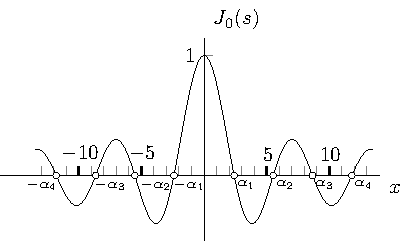
\includegraphics{figOctaveBesselFunctionFirstKind}
\caption{بیسل تفاعل $J_0(s)$}
\label{شکل_جزوی_بیسل_تفاعل_پہلی_قسم}
\end{figure}

یوں تفاعل
\begin{align}\label{مساوات_جزوی_دائری_حل_پ}
W_m(r)=J_0(k_mr)=J_0\big(\frac{\alpha_m}{R}r\big)\quad \quad \quad m=1,2,\cdots
\end{align}
مساوات \حوالہ{مساوات_جزوی_دائری_جھلی_ج} کا وہ حل ہو گا جو جھلی کی سرحد پر صفر ہے۔

یوں \عددی{\lambda=\lambda_m=ck_m} استعمال کرتے ہوئے مساوات \حوالہ{مساوات_جزوی_دائری_جھلی_ث} کا مطابقتی حل
\begin{align*}
G_m(t)=a_m\cos \lambda_mt+c_2\sin \lambda_mt
\end{align*}
ہو گا۔اس طرح مساوات \حوالہ{مساوات_جزوی_دائری_جھلی_الف} کے ایسے حل جو سرحدی شرط مساوات \حوالہ{مساوات_جزوی_دائری_جھلی_ب} کو مطمئن کرتے ہوں درج ذیل ہوں گے جہاں \عددی{m=1,2,\cdots} ہے۔
\begin{align}\label{مساوات_جزوی_دائری_حل_ت}
u_m(r,t)=W_m(r)G_m(t)=(a_m\cos \lambda_mt+c_2\sin \lambda_mt)J_0(k_mr)
\end{align}
\عددی{u_m(r,t)} اس مسئلے کے امتیازی تفاعل\فرہنگ{امتیازی!تفاعل} ہیں جبکہ \عددی{\lambda_m} مسئلے کے امتیازی اقدار\فرہنگ{امتیازی اقدار} ہیں۔

ارتعاش کی \عددی{u_m} حصہ  کو \اصطلاح{\عددی{m} ویں عمودی انداز}\فرہنگ{$m^{th}$ normal mode}\حاشیہب{$m^{th}$ normal mode}\فرہنگ{normal mode} کہتے ہیں جس کی تعدد \عددی{\tfrac{\lambda_m}{2\pi}} چکر فی اکائی وقت ہو گی۔ \عددی{x} محور پر سائن تفاعل کے صفروں کے درمیان یکساں فاصلہ پایا جاتا ہے  جبکہ \عددی{J_0} کے صفروں کے درمیان یکساں فاصلہ نہیں پایا جاتا ہے۔یہی وجہ ہے کہ ستار کی ترنگ اور طبلہ کی تھاپ  مختلف ہیں۔شکل میں دکھائے گئے جھلی کی عمودی انداز شکل \حوالہ{شکل_جزوی_بیسل_تفاعل_پہلی_قسم} سے با آسانی حاصل کیے جا سکتے ہیں (شکل \حوالہ{شکل_جزوی_دائری_عمودی_انداز})۔عمودی انداز \عددی{m=1} میں پوری جھلی بیک وقت اوپر (یا نیچے) حرکت کرتی ہے۔\عددی{m=2} کے لئے تفاعل
\begin{align*}
W_2(r)=J_0\big(\frac{\alpha_2}{R}r\big)
\end{align*}
ان نقطوں پر صفر ہو گا جہاں  \عددی{\tfrac{\alpha_2r}{R}=\alpha_1} یعنی \عددی{r=\tfrac{\alpha_1R}{\alpha_2}} ہو۔ یوں \عددی{r=\tfrac{\alpha_1R}{\alpha_2}} صفر ہٹاو لکیر ہو گی جس کو شکل \حوالہ{شکل_جزوی_دائری_عمودی_انداز} میں نقطہ دار لکیر سے دکھایا گیا ہے۔اب جن لمحات پر جھلی کا وسطی خطہ اوپر حرکت کرتا ہے ان لمحات پر جھلی کا بیرونی خطہ \عددی{r>\tfrac{\alpha_1R}{\alpha_2}} نیچے کو حرکت کرے گا اور اسی طرح جب وسطی خطہ نیچے کو حرکت کرتا ہے تب بیرونی خطہ اوپر کو حرکت کرتا ہے۔حل \عددی{u_m(r,t)} کے \عددی{m-1} عدد صفر ہٹاو لکیریں ہوں گی (شکل \حوالہ{شکل_جزوی_دائری_عمودی_انداز}) جو ہم مرکز دائرے ہوں گے۔
%  
\begin{figure}
\centering
\begin{subfigure}{0.33\textwidth}
\centering
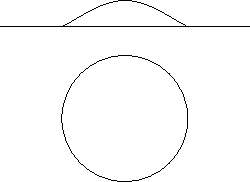
\includegraphics{figOctaveCircularMembraneNormalModesOne}
\end{subfigure}%
\begin{subfigure}{0.33\textwidth}
\centering
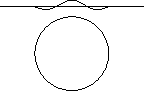
\includegraphics{figOctaveCircularMembraneNormalModesTwo}
\end{subfigure}%
\begin{subfigure}{0.33\textwidth}
\centering
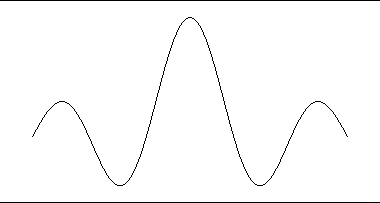
\includegraphics{figOctaveCircularMembraneNormalModesThree}
\end{subfigure}%
\caption{زاویہ سے آزاد دائری جھلی کی عمودی انداز}
\label{شکل_جزوی_دائری_عمودی_انداز}
\end{figure}

%

\موٹا{تیسرا قدم۔} \quad ایسا حل جو ابتدائی شرائط مساوات \حوالہ{مساوات_جزوی_دائری_جھلی_پ} اور مساوات \حوالہ{مساوات_جزوی_دائری_جھلی_ت} کو مطمئن کرتا ہو حاصل کرنے کی خاطر ہم ارتعاش پذیر تار کے حل کی طرح آگے بڑھتے ہیں یعنی ہم درج ذیل تسلسل پر غور کرتے ہیں۔\حاشیہد{ہم یکتائی اور ارتکاز کے مسئلے پر یہاں غور نہیں کریں گے۔}
\begin{align}\label{مساوات_جزوی_دائری_حل_ٹ}
u(r,t)=\sum_{m=1}^{\infty} W(r)G_m(t)=\sum_{m=1}^{\infty} (a_m\cos\lambda_mt+b_m\sin\lambda_mt)J_o\big(\frac{\alpha_m}{R}r\big)
\end{align}
اس میں \عددی{t=0} پر کرتے ہوئے  اور مساوات \حوالہ{مساوات_جزوی_دائری_جھلی_پ} استعمال کرتے ہوئے 
\begin{align}\label{مساوات_جزوی_دائری_حل_ث}
u(r,0)=\sum_{m=1}^{\infty} a_mJ_0\big(\frac{\alpha_m}{R}r\big)=f(r)
\end{align}
ملتا ہے۔یوں اگر مساوات \حوالہ{مساوات_جزوی_دائری_حل_ٹ} نے \حوالہ{مساوات_جزوی_دائری_جھلی_پ} کو مطمئن کرنا ہو تب \عددی{a_m}، تفاعل \عددی{f(r)} کی بیسل تسلسل  کے عددی سر ہوں گے۔یہ تسلسل \عددی{J_0(\tfrac{\alpha_m}{R}r)} کی صورت میں ہو گی۔یوں صفحہ \حوالہصفحہ{مساوات_طاقتی_فوریئر_بیسل_عددی_سر} پر مساوات \حوالہ{مساوات_طاقتی_فوریئر_بیسل_عددی_سر} کے تحت
\begin{align}\label{مساوات_جزوی_دائری_حل_ج}
a_m=\frac{2}{R^2J^2_1(\alpha_{m})}\int_0^R rf(r)J_0(\frac{\alpha_m}{R}r)\dif r\quad \quad m=1,2,
\end{align}
ہوں گے۔ وقفہ \عددی{0\le r\le R} پر \عددی{f(r)} کا قابل تفرق ہونا مساوات \حوالہ{مساوات_جزوی_دائری_حل_ث} کی صورت میں \عددی{f(r)} کی تسلسل لکھنے کے لئے کافی شرط ہے۔مساوات \حوالہ{مساوات_جزوی_دائری_حل_ٹ} میں عددی سر \عددی{b_m} کو مساوات \حوالہ{مساوات_جزوی_دائری_جھلی_ت} سے اسی طرح  حاصل کیا جا سکتا ہے۔
\begin{align}\label{مساوات_جزوی_دائری_حل_چ}
b_m=\frac{2}{c\alpha_m RJ_1^2(\alpha_m)}\int_0^R rg(r)J_0\big(\frac{\alpha_m}{R}r\big)\,\dif r,\quad \quad m=1,2,\cdots
\end{align}
\عددی{a_m} اور \عددی{b_m} کی اعدادی قیمتیں حاصل کرنے کی خاطر ہم \عددی{J_0} اور \عددی{J_1} کی قیمتوں کے جدول استعمال کرتے ہوئے تکمل کا تخمینہ لگائیں گے۔

%=========================
\حصہء{سوالات}

%==========================
\ابتدا{سوال}\quad
\عددی{R=1} لیتے ہوئے \عددی{u_2} اور \عددی{u_3} کی صفر ہٹاو دائروں کی رداس تلاش کریں (مساوات \حوالہ{مساوات_جزوی_دائری_حل_ت})۔\\
جواب:\quad
$u_2:r=\tfrac{\alpha_1}{\alpha_2}R=0.43565,\quad u_3:r=\tfrac{\alpha_1}{\alpha_3}R=0.27789, \quad r=\tfrac{\alpha_2}{\alpha_3}R=0.63788$
\انتہا{سوال}
%===========================
\ابتدا{سوال}\quad
\عددی{R=1} لیتے ہوئے \عددی{u_4} کی صفر ہٹاو دائروں کی رداس تلاش کریں۔\\
جواب:\quad
$0.20394, \quad 0.46814,\quad 0.73389$
\انتہا{سوال}
%==========================
\ابتدا{سوال}\quad
شکل \حوالہ{شکل_جزوی_دائری_عمودی_انداز} کی طرح اشکال \عددی{u_4} اور \عددی{u_5} کے لئے کھینچیں۔
\انتہا{سوال}
%======================
\ابتدا{سوال}\quad
جھلی میں تناو بڑھانے سے مختلف عمودی انداز (مساوات \حوالہ{مساوات_جزوی_دائری_حل_ت}) کی تعدد پر کیا اثر پڑتا ہے؟\\
جواب:\quad تناو بڑھنے سے \عددی{c} بڑھتا ہے لہٰذا تعدد بڑھے گی۔
\انتہا{سوال}
%==========================
\ابتدا{سوال}\quad 
مساوات \حوالہ{مساوات_جزوی_دائری_حل_چ} حاصل کریں۔
\انتہا{سوال}
%================
\ابتدا{سوال}\quad
کیا مقررہ \عددی{c} اور \عددی{R} کی صورت میں دو یا دو سے زیادہ تفاعل \عددی{u_m} (مساوات \حوالہ{مساوات_جزوی_دائری_حل_ت}) جن کے صفر ہٹاو لکیریں مختلف ہوں کا ایک ہی امتیازی قدر ہو سکتا ہے؟
\انتہا{سوال}
%===================
\ابتدا{سوال}\شناخت{سوال_جزوی_مکمل_آزاد_ارتعاش_جھلی}\quad \موٹا{قطبی محدد کے ($r$ اور $\theta$ پر منحصر) ارتعاش}\\
مساوات موج
\begin{align}\label{مساوات_جزوی_سوال_الف}
u_{tt}=c^2\big(u_{rr}+\frac{1}{r}u_r+\frac{1}{r^2}u_{\theta \theta}\big)
\end{align}
 میں \عددی{u=F(r,\theta)G(t)} پر کرتے ہوئے درج ذیل حاصل کریں۔
\begin{align}
\ddot{G}+\lambda^2G=0,\quad \quad \lambda=ck\label{مساوات_جزوی_سوال_ب}\\
F_{rr}+\frac{1}{r}F_r+\frac{1}{r^2}F_{\theta\theta}+k^2F=0\label{مساوات_جزوی_سوال_پ}
\end{align}
\انتہا{سوال}
%=========================
\ابتدا{سوال}\quad
مساوات \حوالہ{مساوات_جزوی_سوال_پ} میں \عددی{F=W(r)Q(\theta)} پر کرتے ہوئے درج ذیل حاصل کریں۔
\begin{align}
Q''+n^2Q=0\label{مساوات_جزوی_سوال_ت}\\
r^2W''+rW'+(k^2r^2-n^2)W=0\label{مساوات_جزوی_سوال_ٹ}
\end{align}
\انتہا{سوال}
%=========================
\ابتدا{سوال}\quad
وضاحت کریں کہ \عددی{Q(\theta)} دوری ہو گا جس کا دوری عرصہ \عددی{2\pi} ہو گا لہٰذا مساوات \حوالہ{مساوات_جزوی_سوال_ت} اور مساوات \حوالہ{مساوات_جزوی_سوال_ٹ} میں \عددی{n=0,1,2,\cdots} ہوں گے۔یوں درج ذیل حل حاصل کریں۔
\begin{align}
Q_n=\cos n\theta, \quad Q^*_n=\sin n\theta\label{مساوات_جزوی_سوال_ث}\\
W_n=J_n(kr),\quad n=0,1,\cdots\label{مساوات_جزوی_سوال_ج}
\end{align}
\انتہا{سوال}
%========================
\ابتدا{سوال}\quad
واضح کریں کہ سرحدی شرط
\begin{align}\label{مساوات_جزوی_سوال_چ}
u(R,\theta,t)=0
\end{align}
سے \عددی{k=k_{mn}=\tfrac{\alpha_{mn}}{R}} حاصل ہوتا ہے جہاں \عددی{s=\alpha_{mn}} تفاعل \عددی{J_n(s)} کا مثبت \عددی{m} واں جذر ہے۔
\انتہا{سوال}
%=====================
\ابتدا{سوال}\quad
واضح کریں کہ مساوات \حوالہ{مساوات_جزوی_سوال_الف} کے وہ حل جو مساوات \حوالہ{مساوات_جزوی_سوال_چ} کو مطمئن کرتے ہوں درج ذیل ہیں۔
\begin{gather}
\begin{aligned}\label{مساوات_جزوی_سوال_ح}
u_{mn}&=(A_{mn}\cos ck_{mn}t+B_{mn}\sin ck_{mn}t)J_n(k_{mn}r)\cos n\theta\\
u^*_{mn}&=(A^*_{mn}\cos ck_{mn}t+B^*_{mn}\sin ck_{mn}t)J_n(k_{mn}r)\sin n\theta
\end{aligned}
\end{gather}
\انتہا{سوال}
%=======================
\ابتدا{سوال}\quad
واضح کریں کہ  \عددی{u^*_{m0}\equiv 0} اور \عددی{u_{m0}}  عین مساوات \حوالہ{مساوات_جزوی_دائری_حل_ت} کے تحت ہیں۔
\انتہا{سوال}
%==========================
\ابتدا{سوال}\quad
واضح کریں کہ \عددی{u_{mn}} کی  \عددی{m+n-1} صفر ہٹاو لکیریں ہوں گی۔
\انتہا{سوال}
%===================
سوال \حوالہ{سوال_جزوی_ترسیم_الف} تا سوال \حوالہ{سوال_جزوی_ترسیم_ب} میں دیے گئے حل کی صفر ہٹاو لکیروں کی ترسیم کھینچیں۔

%=============
\ابتدا{سوال}\شناخت{سوال_جزوی_ترسیم_الف}\quad
$u_{3n},\quad n=1,2,3$
\انتہا{سوال}
%====================
\ابتدا{سوال}\quad
$u_{4n},\quad n=1,2,3$
\انتہا{سوال}
%====================
\ابتدا{سوال}\شناخت{سوال_جزوی_ترسیم_ب}\quad
$u^*_{mn},\quad m,n=1,2,3$\\
جواب:\quad صفر ہٹاو لکیریں شکل \حوالہ{شکل_سوال_جزوی_ترسیم_ب} میں دکھائی گئی ہیں۔
\begin{figure}
\centering
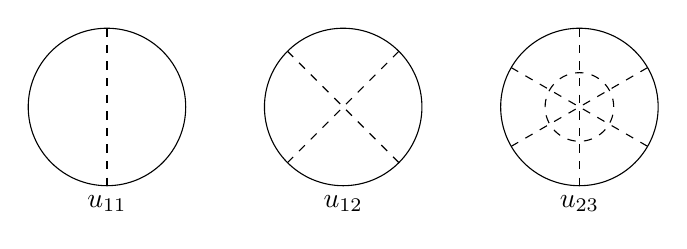
\begin{tikzpicture}
\draw(0,0) circle (1);
\draw[dashed] (0,1)--(0,-1)node[below]{$u_{11}$};
\begin{scope}[xshift={3cm}]
\draw(0,0) circle (1);
\draw[dashed] (0,0)++(45:1)--++(45:-2);
\draw[dashed] (0,0)++(-45:1)--++(-45:-2);
\draw(0,-1)node[below]{$u_{12}$};
\end{scope}
\begin{scope}[xshift={6cm}]
\draw(0,0) circle (1);
\draw[dashed](0,0) circle (0.4356);
\draw[dashed] (0,1)--(0,-1);
\draw[dashed] (0,0)++(30:1)--++(30:-2);
\draw[dashed] (0,0)++(-30:1)--++(-30:-2);
\draw(0,-1)node[below]{$u_{23}$};
\end{scope}
\end{tikzpicture}
\caption{چند صفر ہٹاو لکیریں (سوال \حوالہ{سوال_جزوی_ترسیم_ب})}
\label{شکل_سوال_جزوی_ترسیم_ب}
\end{figure}
\انتہا{سوال}
%====================
\ابتدا{سوال}\quad
ابتدائی معلومات \عددی{u_t(r,\theta,0)} کی صورت میں مساوات \حوالہ{مساوات_جزوی_سوال_ح} سے  \عددی{B_{mn}=0} اور \عددی{B^*_{mn}=0} حاصل کریں۔
\انتہا{سوال}
%=========================
سوال \حوالہ{سوال_جزوی_رفتار_الف} تا سوال \حوالہ{سوال_جزوی_رفتار_ب} میں \عددی{R=1}، \عددی{c=1} اور ابتدائی رفتار صفر لیتے ہوئے،  ابتدائی انحراف \عددی{f(r)} کی صورت میں دائری جھلی کی  انحراف \عددی{u(r,t)} حاصل کریں۔ (اشارہ سوال \حوالہ{سوال_طاقتی_بیسل_فوریئر_تسلسل_الف} تا سوال \حوالہ{سوال_طاقتی_بیسل_فوریئر_تسلسل_ب} پر ایک مرتبہ دوبارہ نظر ڈالیں۔)

%==========
\ابتدا{سوال}\شناخت{سوال_جزوی_رفتار_الف}\quad
$f=0.1J_0(\alpha_2r)$
\انتہا{سوال}
%==========================
\ابتدا{سوال}\quad
$f=k(1-r^2)$\\
جواب:\quad
$u=4k\sum_{m=1}^{\infty}\frac{J_2(\alpha_m)}{\alpha_m^2J_1^2(\alpha_m)}\cos \alpha_m t\,J_0(\alpha_m r)$
\انتہا{سوال}
%==========================
\ابتدا{سوال}\شناخت{سوال_جزوی_رفتار_ب}\quad
$f=k(1-r^4)$
\انتہا{سوال}
%==========================

\حصہ{مساوات لاپلاس۔ نظریہ مخفی قوہ}\شناخت{حصہ_جزوی_مخفی_قوہ}
طبیعیات کی اہم ترین مساوات میں سے ایک درج ذیل مساوات لاپلاس  ہے
\begin{align}\label{مساوات_جزوی_لاپلاس_الف}
\nabla^{\,2}u=0
\end{align}
جہاں \عددی{u} کا لاپلاسی  \عددی{\nabla^{\,2}u}  ہے۔کارتیسی محدد \عددی{x}، \عددی{y}، \عددی{z} میں
\begin{align}\label{مساوات_جزوی_لاپلاس_ب}
\nabla^{\,2}u=\frac{\partial^{\,2}u}{\partial x^2}+\frac{\partial^{\,2}u}{\partial y^2}+\frac{\partial^{\,2}u}{\partial z^2}
\end{align}
ہو گا۔مساوات لاپلاس کے نظریہ کو \اصطلاح{نظریہ مخفی قوہ}\فرہنگ{نظریہ مخفی قوہ}\حاشیہب{potential theory}\فرہنگ{potential theory} کہتے ہیں۔مساوات \حوالہ{مساوات_جزوی_لاپلاس_الف} کے ایسے حل جن کے دو درجی تفرقات استمراری ہوں \اصطلاح{ہارمونی تفاعل}\فرہنگ{ہارمونی!تفاعل}\حاشیہب{harmonic functions}\فرہنگ{harmonic!functions} کہلاتے ہیں۔

دو ابعادی صورت جہاں \عددی{u} صرف دو عدد متغیرات کے تابع ہو کا مخلوط تجزیہ زیادہ آسان ثابت ہوتا ہے لہٰذا اس پر اگلے باب میں غور کیا جائے گا۔

انجینئری حساب میں مساوات لاپلاس کی اہمیت واضح کرنے کی خاطر چند مثالوں کا ذکر کرتے ہیں۔

مساوات لاپلاس ثقلی میدان کے مسائل میں سامنے آتی ہے۔  مثلاً صفحہ \حوالہصفحہ{مثال_الاحصاء_ثقلی_میدان} پر مثال \حوالہ{مثال_الاحصاء_ثقلی_میدان} میں ہم نے دیکھا کہ اگر ایک ذرہ \عددی{A} جس کی کمیت \عددی{M} ہو نقطہ \عددی{(\xi,\eta,\zeta)} پر مستقل موجود ہو اور دوسرا ذرہ \عددی{B} جس کی کمیت \عددی{m} ہو نقطہ \عددی{(x,y,z)} پر موجود ہو تب \عددی{A} ذرہ \عددی{B} کو اپنی جانب کھینچے گا۔یہ ثقلی قوت درج ذیل غیر سمتی تفاعل \عددی{u(x,y,z)} کی ڈھلوان ہے۔
\begin{align*}
u(x,y,z)=\frac{GMm}{r}\\
r=\sqrt{(x-\xi)^2+(y-\eta)^2+(z-\zeta)^2}\quad (>0)
\end{align*}
تفاعل \عددی{u(x,y)} کو ثقلی میدان کی \اصطلاح{مخفی قوہ} کہتے ہیں اور یہ لاپلاس کی مساوات کو مطمئن کرتا ہے۔ 

نقطہ کمیت کی مخفی قوہ اور قوت کی تصور کو مسلسل کمیت کے لئے بیان کرتے ہیں۔اگر خطہ \عددی{R} میں کمیتی کثافت \عددی{\rho(\xi,\eta,\zeta)} پائی جاتی ہو تب  نقطہ \عددی{(x,y,z)} جہاں کمیت موجود نہ ہو  پر مخفی قوہ \عددی{u} درج ذیل ہو گی۔ 
\begin{align}\label{مساوات_جزوی_لاپلاس_پ}
u(x,y,z)=k\iiint\limits_R \frac{\rho}{r}\dif \xi\,\dif \eta\,\dif \zeta\quad \quad \quad (k>0)
\end{align}
چونکہ \عددی{\frac{1}{r} (r>0)} مساوات \حوالہ{مساوات_جزوی_لاپلاس_الف} کا حل ہے لہٰذا \عددی{\nabla^{\,2}(\tfrac{1}{r})=0} ہو گا اور کثافت \عددی{\rho}  متغیرات \عددی{x}، \عددی{y}، \عددی{z} پر منحصر نہیں ہے لہٰذا درج ذیل حاصل ہوتا ہے۔
\begin{align*}
\nabla^{\,2}u=k\iiint\limits_R \rho\nabla^{\,2}\big(\frac{1}{r}\big) \dif \xi\,\dif \eta\,\dif \zeta=0
\end{align*}
یوں مساوات \حوالہ{مساوات_جزوی_لاپلاس_پ} میں دی گئی ثقلی مخفی قوہ مساوات لاپلاس کو ہر اس نقطہ پر مطمئن کرتی ہے جہاں پر کمیت موجود نہ ہو۔

برقی سکون کی میدان میں برقی بار کے مابین قوت کشش یا قوت دفع قانون کولمب دیتی ہے جس کی ریاضی شکل عین نیوٹن کے قانون ثقل کی طرح ہے۔یوں ہم اخذ کر سکتے ہیں کہ جس نقطہ پر برقی بار موجود نہ ہو اس نقطہ پر برقی مخفی قوہ کو ایسے تفاعل سے ظاہر کیا جا سکتا  ہے جو برقی بار سے پاک نقطہ پر لاپلاس کی مساوات کو مطمئن کرتا ہو۔

ہم بعد کے باب میں دیکھیں گے کہ غیر  داب پذیر سیال کی بہاو پر غور کے دوران بھی لاپلاس مساوات  سامنے آتی ہے۔

مزید حرارت کے مسائل میں حراری مساوات
\begin{align*}
u_t=c^2\nabla^{\,2}u
\end{align*}
 بنیادی اہمیت رکھتی ہے۔اگر درجہ حرارت وقت \عددی{t} کے تابع نہ ہو (برقرار حالت) تب یہ لاپلاس مساوات کی صورت اختیار کرتی ہے۔
\begin{figure}
\centering
\begin{subfigure}{0.5\textwidth}
\centering
\begin{tikzpicture}
\draw(0,0)--++(2,0)node[right]{$y$};
\draw(0,0)--++(-110:1.5)node[left]{$x$};
\draw(0,0)--++(0,1.5)node[left]{$z$};
%
\draw[-stealth]([shift={(-110:0.3)}]0,0) arc (-110:-45:0.3);
\draw[dashed] (0,0)--++(-45:1.5)coordinate(kA)node[pos=0.5,below,solid]{$\rho$};
\draw[dashed](kA)--++(0,2)node[solid,ocirc]{}node[right]{$(\rho,\phi,z)$};
\RightAngle{(0,0)}{(kA)}{(0,2)};
\draw(-80:0.6)node[]{$\phi$};
\end{tikzpicture}
\caption*{(الف) نلکی محدد}
\end{subfigure}%
\begin{subfigure}{0.5\textwidth}
\centering
\begin{tikzpicture}[]
\draw(0,0)--++(2,0)node[right]{$y$};
\draw[name path=kX](0,0)--++(-110:1.5)node[left]{$x$};
\draw(0,0)--++(0,2.5)node[left]{$z$};
%
\draw[-stealth]([shift={(-110:0.3)}]0,0) arc (-110:-45:0.3);
\draw[dashed] (0,0)--++(-45:1.5)coordinate(kA);
\draw[dashed](kA)--++(0,2)node[right]{$(r,\phi,z)$}coordinate(kB);
\draw(-80:0.6)node[]{$\phi$};
\draw[thick](0,0)--(kB);
\draw[dashed] (kB)node[ocirc,solid]{}--++(-45:-1.5)coordinate(kC)node[pos=0.5,rotate=-45,above]{$r\sin \theta$};
\RightAngle{(kB)}{(kC)}{(0,0)};
\RightAngle{(0,0)}{(kA)}{(0,2)};
%
\draw[-stealth]([shift={(90:0.5)}]0,0) arc (90:45:0.5);
\draw(70:0.8)node{$\theta$};
%
\path[name path=kXX] (kA)--++(-2,0);
\draw[dashed,name intersections={of=kX and kXX}] (kA)--(intersection-1)coordinate(kI);
\RightAngle{(kA)}{(kI)}{(0,0)};
%
\draw [decorate,decoration={brace,amplitude=5pt},xshift=-4pt,yshift=0pt](kI)++(-0.2,0) --++(70:1.2) node [black,midway,xshift=-0.3cm,yshift=0.2cm,rotate=70] {\footnotesize $r\sin\theta\cos\phi$};
\end{tikzpicture}
\caption*{(ب) کروی محدد}
\end{subfigure}%
\caption{نلکی اور کروی محدد کی تعریف}
\label{شکل_جزوی_نلکی_کروی}
\end{figure}

عموماً مسائل، جن میں لاپلاس مساوات حاصل ہو گی، میں \اصطلاح{سرحدی قیمت مسئلہ}\فرہنگ{سرحدی!قیمت مسئلہ}\حاشیہب{boundary value problem}\فرہنگ{boundary!value problem} حل کرنا ہو گا جہاں مساوات \حوالہ{مساوات_جزوی_لاپلاس_الف} کا ایسا حل درکار ہو گا جو کسی سرحد پر دیا گیا شرط مطمئن کرتا ہو۔یوں خلا میں ایسے محدد متعارف کرنا ضروری ہو گا جن میں اس سرحد کو بیان کرنا آسان  ہو۔اس طرح مساوات \حوالہ{مساوات_جزوی_لاپلاس_ب} کے لاپلاسی کا تبادلہ ان محدد میں کرنا ہو گا۔ہم حصہ \حوالہ{حصہ_جزوی_قطبی_محدد_لاپلاسی} میں دو متغیرات کے تفاعل کی لاپلاسی کا تبادلہ کر چکے ہیں۔ایک محدد سے دوسرے محدد میں لاپلاسی کا تبادلہ اسی طرح کیا جائے گا۔

نلکی محدد میں لاپلاسی صفحہ \حوالہصفحہ{مساوات_جزوی_لاپلاسی_نلکی_محدد} پر مساوات \حوالہ{مساوات_جزوی_لاپلاسی_نلکی_محدد} دیتی ہے۔نلکی محدد (شکل \حوالہ{شکل_جزوی_نلکی_کروی}-الف) کی تعریف
\begin{align}\label{مساوات_جزوی_تعریف_محددی_نظام_الف}
\rho&=\sqrt{x^2+y^2}, \quad \phi=\tan^{-1}\frac{y}{x},\quad z=z
\end{align}
 اور اس میں لاپلاسی کو یہاں دوبارہ پیش کرتے ہیں۔
\begin{align}\label{مساوات_جزوی_تعریف_محددی_نظام_ب}
\nabla^{\,2}u=&\frac{\partial^{\,2}u}{\partial \rho^2}+\frac{1}{\rho}\frac{\partial u}{\partial \rho}+\frac{1}{\rho^2}\frac{\partial^{\,2}u}{\partial \phi^2}+\frac{\partial^{\,2}u}{\partial z^2}
\end{align}

صفحہ \حوالہصفحہ{مساوات_جزوی_کروی_لاپلاسی_الف} پر مساوات \حوالہ{مساوات_جزوی_کروی_لاپلاسی_الف} کروی محدد میں لاپلاسی دیتی ہے۔کروی محدد (شکل \حوالہ{شکل_جزوی_نلکی_کروی}-ب) کی تعریف
\begin{align}\label{مساوات_جزوی_تعریف_محددی_نظام_پ}
x&=r\sin\theta\cos\phi,\quad y=r\sin\theta\sin\phi,\quad z=r\sin\theta
\end{align}
 اور اس میں لاپلاسی کو یہاں دوبارہ پیش کرتے ہیں
\begin{align}\label{مساوات_جزوی_تعریف_محددی_نظام_ت}
\nabla^{\,2}u=u_{rr}+\frac{2}{r}u_r+\frac{1}{r^2}u_{\theta\theta}+\frac{\cot \theta}{r^2}u_{\theta}+\frac{1}{r^2\sin^2\theta}u_{\phi\phi}
\end{align}
جس کو درج ذیل بھی لکھا جا سکتا ہے۔
\begin{align}\label{مساوات_جزوی_تعریف_محددی_نظام_ٹ}
\nabla^{\,2}u=\frac{1}{r^2}\big[\frac{\partial}{\partial r}\big(r^2\frac{\partial u}{\partial r}\big)+\frac{1}{\sin \theta}\frac{\partial}{\partial \theta}\big(\sin \theta \frac{\partial u}{\partial \theta}\big)+\frac{1}{\sin^2\theta} \frac{\partial^{\,2}u}{\partial \phi^2}\big]
\end{align}

%=====================
\حصہء{سوالات}

%==============
\ابتدا{سوال}\quad
محدد \عددی{x^*=ax}، \عددی{y^*=by}، \عددی{z^*=cz} میں لاپلاسی حاصل کریں جہاں \عددی{x}، \عددی{y}، \عددی{z} کارتیسی محدد ہیں۔\\
جواب:\quad
$a^2u_{x^*x^*}+b^2u_{y^*y^*}+c^2u_{z^*z^*}$
\انتہا{سوال}
%=========================
\ابتدا{سوال}\quad
مساوات \حوالہ{مساوات_جزوی_لاپلاس_ب} سے شروع کرتے ہوئے 
صفحہ \حوالہصفحہ{مساوات_الاحصاء_عمومی_مستوی_تبادل_الف} پر مساوات \حوالہ{مساوات_الاحصاء_عمومی_مستوی_تبادل_الف} اور مساوات \حوالہ{مساوات_الاحصاء_عمومی_مستوی_تبادل_ب} استعمال کرتے ہوئے درج ذیل حاصل کریں۔
\begin{align*}
\nabla^{\,2}u=u_{x^*x^*}+u_{y^*y^*}+u_{z^*z^*}
\end{align*}
\انتہا{سوال}
%===================
تصدیق کریں کہ سوال \حوالہ{سوال_جزوی_تصدیق_لاپلاس_حل_الف} تا سوال \حوالہ{سوال_جزوی_تصدیق_لاپلاس_حل_ب} میں تفاعل \عددی{u=f(x,y)}  مساوات لاپلاس کو مطمئن کرتا ہے۔چند ہم قوہ خطوط \عددی{u=c} جہاں \عددی{c} مستقل ہے کی ترسیم کھینچیں۔

%====================
\ابتدا{سوال}\شناخت{سوال_جزوی_تصدیق_لاپلاس_حل_الف}\quad
$x^2-y^2$
\انتہا{سوال}
%=========================
\ابتدا{سوال}\quad
$x^3-3xy^2$
\انتہا{سوال}
%=========================
\ابتدا{سوال}\quad
$\tfrac{x}{x^2+y^2}$
\انتہا{سوال}
%=========================
\ابتدا{سوال}\quad
$\tfrac{y}{x^2+y^2}$
\انتہا{سوال}
%=========================
\ابتدا{سوال}\شناخت{سوال_جزوی_تصدیق_لاپلاس_حل_ب}\quad
$\tfrac{x^2-y^2}{(x^2+y^2)^2}$
\انتہا{سوال}
%=========================
\ابتدا{سوال}\quad
کارتیسی نظام محدد استعمال کرتے ہوئے مساوات \حوالہ{مساوات_جزوی_تعریف_محددی_نظام_پ} میں کروی محدد کی تعریف بیان کی گئی ہے۔ان مساوات کو استعمال کرتے ہوئے کارتیسی نظام کی تعریف کروی محددی نظام میں کریں۔\\
جواب:\quad
$r=\sqrt{x^2+y^2+z^2},\quad \theta=\tan^{-1}\frac{z}{\sqrt{x^2+y^2+z^2}},\quad \phi=\tan^{-1}\frac{y}{x}$
\انتہا{سوال}
%==========================
\ابتدا{سوال}\quad
مساوات \حوالہ{مساوات_جزوی_تعریف_محددی_نظام_ب} سے واپس کارتیسی محدد میں لاپلاسی حاصل کریں۔
\انتہا{سوال}
%==========================
\ابتدا{سوال}\quad
تصدیق کریں کہ \عددی{u=\tfrac{c}{r}} کروی محدد میں لاپلاسی کو مطمئن کرتا ہے جہاں \عددی{c} مستقل ہے۔
\انتہا{سوال}
%====================
\ابتدا{سوال}\شناخت{سوال_جزوی_لاپلاس_رداس_تابع_حل_الف}\quad
لاپلاس مساوات \عددی{\nabla^{\,2}u=0} کا ایسا حل تلاش کریں جو صرف \عددی{r=\sqrt{x^2+y^2+z^2}} کا تابع ہو۔\\
جواب:\quad اگر \عددی{u} صرف \عددی{r} کا تابع ہو تب مساوات  \حوالہ{مساوات_جزوی_تعریف_محددی_نظام_ٹ} کی صورت 
$\tfrac{1}{r^2}\big[\tfrac{\partial}{\partial r}\big(r^2\tfrac{\partial u}{\partial r}\big)\big]=0$
 یعنی
$ \tfrac{\partial}{\partial r}\big(r^2\tfrac{\partial u}{\partial r}\big)=0$
ہو گی جہاں جزوی تفرق کی جگہ تفرق لکھا گیا ہے۔اس کا تکمل \عددی{r^2\tfrac{\partial u}{\partial r}=c}ہو گا جس کو \عددی{\dif u=\tfrac{c}{r^2}\dif r} لکھ کر تکمل لینے سے درکار حل \عددی{u=k-\tfrac{c}{r}} حاصل ہو گا جہاں \عددی{c} اور \عددی{k} مستقل ہیں۔
\انتہا{سوال}
%======================
\ابتدا{سوال}\شناخت{سوال_جزوی_لاپلاس_رداس_تابع_حل_ب}\quad دو ہم مرکز کرہ کے رداس \عددی{r_1=\SI{15}{\centi\meter}} اور \عددی{r_2=\SI{1}{\centi\meter}} ہیں جبکہ ان پر برقی دباو بالترتیب \عددی{U_1=\SI{1000}{\volt}} اور \عددی{U_2=\SI{100}{\volt}} ہے۔ہم مرکز کرہ کے درمیان خطہ میں ساکن برقی دباو \عددی{u} سوال \حوالہ{سوال_جزوی_لاپلاس_رداس_تابع_حل_الف} میں حاصل کی گئی۔موجودہ معلومات کو استعمال کرتے ہوئے \عددی{c} اور \عددی{k} دریافت کریں اور حاصل \عددی{u} کی ترسیم کھینچیں۔\\
جواب:\quad
$u=\tfrac{7450}{7}-\tfrac{135}{14 r}$
\انتہا{سوال}
%====================
\ابتدا{سوال}\شناخت{سوال_جزوی_نلکی_لاپلاس_حل_الف}\quad
دو ابعادی لاپلاس مساوات جو صرف \عددی{\rho=\sqrt{x^2+y^2}} کے تابع ہو کا حل تلاش کریں۔\\
جواب:\quad اگر \عددی{u} صرف \عددی{\rho} کا تابع ہو تب مساوات \حوالہ{مساوات_جزوی_تعریف_محددی_نظام_ب} کی صورت
$\frac{\dif^{\,2}u}{\dif \rho^2}+\frac{1}{\rho}\frac{\dif u}{\dif \rho}=0$
ہو گی جہاں جزوی تفرق کی جگہ تفرق لکھا گیا ہے۔اس میں \عددی{v=\tfrac{\dif u}{\dif \rho}} پر کرتے ہوئے \عددی{\tfrac{\dif v}{\dif \rho}+\tfrac{v}{\rho}=0} یعنی \عددی{\tfrac{\dif v}{v}=-\tfrac{\dif \rho}{\rho}} حاصل ہوتا ہے جس کا  تکمل \عددی{v\rho=c} یعنی 
\عددی{\tfrac{\partial u}{\partial \rho}=\tfrac{c}{\rho}} دیتا ہے۔درکار جواب تکمل لینے سے \عددی{u=k+c\ln \rho} حاصل ہوتا ہے جہاں \عددی{c} اور \عددی{k} مستقل ہیں۔
\انتہا{سوال}
%========================
\ابتدا{سوال}\شناخت{سوال_جزوی_نلکی_لاپلاس_حل_ب}\quad 
دو ہم محور نلکیوں کا رداس \عددی{\rho_1=\SI{5}{\centi\meter}} اور \عددی{\rho_2=\SI{20}{\centi\meter}} ہے جبکہ ان پر برقی دباو بالترتیب
 \عددی{U_1=\SI{10}{\volt}} اور \عددی{U_2=\SI{60}{\volt}} ہے۔ سوال \حوالہ{سوال_جزوی_نلکی_لاپلاس_حل_الف} میں حاصل حل استعمال کرتے ہوئے نلکیوں کے درمیان خطہ میں برقی دباو کی مساوات حاصل کریں۔ حاصل \عددی{u} کی ترسیم کھینچیں۔موجودہ ترسیم کا سوال \حوالہ{سوال_جزوی_لاپلاس_رداس_تابع_حل_ب} میں حاصل کردہ ترسیم کے ساتھ موازنہ کریں۔\\
جواب:\quad
$u=118.048+36.067\ln \rho$
\انتہا{سوال}
%======================
\ابتدا{سوال}\quad
اگر کروی محدد میں \عددی{u(r,\theta,\phi)} مساوات لاپلاس \عددی{\nabla^{\,2}u=0} کو مطمئن کرتا ہو تب ثابت کریں کہ \عددی{v(r,\theta,\phi)=r^{-1}u(r^{-1},\theta,\phi)} مساوات \عددی{\nabla^{\,2}v=0} کو مطمئن کرے گا۔
\انتہا{سوال}
%======================
\ابتدا{سوال}\quad
مساوات موج \عددی{u_{tt}=c^2\nabla^{\,2}u} میں \عددی{u=U(x,y,z)e^{-i\omega t}} پر کرتے ہوئے درج ذیل \اصطلاح{مساوات ہلم ہولٹز}\فرہنگ{مساوات!ہلم ہولٹز}\فرہنگ{ہلم ہولٹز!مساوات}\حاشیہب{Helmholtz equation}\فرہنگ{Helmholtz equation} حاصل\حاشیہد{جرمن ماہر طبیعیات ہرمن لڈوگ فرڈینانڈ ون ہلم ہولٹز [1821-1894]} کریں جہاں \عددی{i=\sqrt{-1}} ہے۔
\begin{align*}
\nabla^{\,2}U+k^2U=0\quad \quad \quad k=\frac{\omega}{c}
\end{align*}
\انتہا{سوال}
%====================
سوال \حوالہ{سوال_جزوی_برقرار_حال_الف} تا سوال \حوالہ{سوال_جزوی_برقرار_حال_الف} میں برقرار حال (وقت کا غیر تابع) درجہ حرارت \عددی{u} تلاش کریں۔

%====================
\ابتدا{سوال}\شناخت{سوال_جزوی_برقرار_حال_الف}\quad
دو متوازی چادر \عددی{x=x_0} اور \عددی{x=x_1} کے درمیان جنہیں بالترتیب \عددی{u_0} اور \عددی{u_1} درجہ حرارت پر برقرار رکھا گیا ہے۔\\
جواب:\quad
$u=\tfrac{(u_1-u_0)x}{x_1-x_0}+\tfrac{u_0x_1-u_1x_0}{x_1-x_0}$
\انتہا{سوال}
%========================
\ابتدا{سوال}\quad
دو ہم محور نلکیوں \عددی{\rho=\rho_1} اور \عددی{\rho=\rho_2} کے درمیان جنہیں بالترتیب \عددی{u_0} اور \عددی{u_1} درجہ حرارت پر برقرار رکھا گیا ہے۔\\
جواب:\quad
$u=\tfrac{u_1-u_0}{\ln \tfrac{r_1}{r_0}}\ln r+\tfrac{u_0\ln r_1-u_1\ln r_0}{\ln \tfrac{r_1}{r_0}}$
\انتہا{سوال}
%========================
\ابتدا{سوال}\quad
دو ہم مرکز کرہ  \عددی{r=r_1} اور \عددی{r=r_2} کے درمیان جنہیں بالترتیب \عددی{u_0} اور \عددی{u_1} درجہ حرارت پر برقرار رکھا گیا ہے۔\\
جواب:\quad
$u=u_0-\tfrac{r_1r_0(u_1-u_0)}{(r_1-r_0)r}$
\انتہا{سوال}
%========================

\حصہ{کروی محدد میں مساوات لاپلاس۔مساوات لیژانڈر}
آئیں ایک ایسے مسئلے پر غور کرتے ہیں جس میں، کروی محدد میں لکھی گئی، مساوات لاپلاس استعمال ہو گی۔فرض کریں کہ کروی محدد کی مرکز پر موجود رداس \عددی{R} کی کرہ \عددی{S} کی سطح کو  برقی دباو 
\begin{align}\label{مساوات_جزوی_کرہ_بار_بردار_الف}
u(R,\theta,\phi)=f(\theta)
\end{align}
پر برقرار رکھا جاتا ہے جہاں \عددی{r}، \عددی{\theta}، \عددی{\phi} کروی محدد ہیں جبکہ \عددی{f(\theta)} دیا گیا تفاعل ہے۔کروی محدد کی تعریف گزشتہ حصے میں کی گئی ہے۔ ہم باقی پوری فضا، جہاں کوئی برقی بار نہیں پایا جاتا، میں برقی دباو \عددی{u} جاننا چاہتے ہیں۔چونکہ \عددی{S} کی سطح پر برقی دباو \عددی{\phi} سے آزاد ہے لہٰذا باقی فضا میں بھی برقی دباو \عددی{\phi} سے آزاد ہو گا۔یوں \عددی{\tfrac{\partial^{\,2}u}{\partial \phi^{\,2}}=0} ہو گا لہٰذا مساوات لاپلاس  درج ذیل صورت اختیار کرے گی
\begin{align}\label{مساوات_جزوی_کرہ_بار_بردار_ب}
\frac{\partial}{\partial r}\big(r^2\frac{\partial u}{\partial r}\big)+\frac{1}{\sin \theta}\frac{\partial}{\partial \theta}\big(\sin \theta \frac{\partial u}{\partial \theta}\big)=0
\end{align}
جہاں مساوات \حوالہ{مساوات_جزوی_تعریف_محددی_نظام_ٹ} کا سہارا لیا گیا ہے۔اب لامتناہی فاصلہ پر برقی دباو صفر ہو گا یعنی:
\begin{align}\label{مساوات_جزوی_کرہ_بار_بردار_پ}
\lim_{r\to\infty} u(r,\theta)=0
\end{align}
ہم علیحدگی متغیرات کی ترکیب سے مساوات \حوالہ{مساوات_جزوی_کرہ_بار_بردار_الف} کا ایسا حل تلاش کرتے ہیں جو سرحدی شرائط مساوات \حوالہ{مساوات_جزوی_کرہ_بار_بردار_الف} اور مساوات \حوالہ{مساوات_جزوی_کرہ_بار_بردار_پ} کو مطمئن کرتا ہو۔یوں مساوات \حوالہ{مساوات_جزوی_کرہ_بار_بردار_ب} میں
\begin{align}\label{مساوات_جزوی_کرہ_بار_بردار_ت}
u(r,\theta)=G(r)H(\theta)
\end{align}
اور اس کے تفرق پر کر کے \عددی{GH} سے تقسیم کرتے ہیں۔
\begin{align*}
\frac{1}{G}\frac{\dif}{\dif r}\big(r^2\frac{\dif G}{\dif r}\big)=-\frac{1}{H\sin \theta}\frac{\dif}{\dif \theta}\big(\sin \theta \frac{\dif H}{\dif \theta}\big)
\end{align*}
اب تک آپ جان چکے ہوں گے کہ ایسی صورت میں مساوات کے دونوں اطراف کسی ایک مستقل مثلاً \عددی{k} کے برابر ہوں گے۔یوں درج ذیل دو عدد سادہ تفرقی مساوات حاصل ہوتے ہیں
\begin{align}
\frac{1}{\sin\theta}\frac{\dif}{\dif \theta}\big(\sin\theta\frac{\dif H}{\dif \theta}\big)+kH&=0\label{مساوات_جزوی_کرہ_بار_بردار_ٹ}\\
\frac{1}{G}\frac{\dif}{\dif r}\big(r^2\frac{\dif G}{\dif r}\big)&=k\label{مساوات_جزوی_کرہ_بار_بردار_ث}
\end{align}
جہاں دوسری مساوات کو 
\begin{align*}
r^2G''+2rG'-kG=0
\end{align*}
لکھا جا سکتا ہے جو \ترچھا{مساوات کوشی} ہے۔ہم  حصہ \حوالہ{حصہ_دو_یولر_کوشی} سے جانتے ہیں کہ مساوات کوشی کے حل کا روپ \عددی{G=r^{\alpha}} ہو گا۔اگر ہم \عددی{k} کی جگہ مستقل کو \عددی{n(n+1)} لکھیں تب ان حل کی صورت نہایت سادہ حاصل ہو گی۔ایسا کرنے سے 
\begin{align}\label{مساوات_جزوی_کرہ_بار_بردار_ج}
r^2G''+2rG'-n(n+1)G=0
\end{align}
لکھا جائے گا جہاں \عددی{n} اختیاری مستقل ہے۔اس میں \عددی{G=r^{\alpha}} پر کرنے سے
\begin{align*}
[\alpha(\alpha-1)+2\alpha-n(n+1)]r^{\alpha}=0
\end{align*}
ملتا ہے۔قوسین میں بند حصے کے صفر \عددی{\alpha=n} اور \عددی{\alpha=-n-1} ہیں۔یوں مساوات \حوالہ{مساوات_جزوی_کرہ_بار_بردار_ج} کے حل
\begin{align}\label{مساوات_جزوی_کرہ_بار_بردار_چ}
G_n(r)=r^n\quad \text{اور}\quad G^*_n(r)=\frac{1}{r^{n+1}}
\end{align}
ہوں گے۔
 
مساوات \حوالہ{مساوات_جزوی_کرہ_بار_بردار_ٹ} میں \عددی{k=n(n+1)} متعارف کر کے ہم 
\begin{align*}
\cos \theta=w
\end{align*}
لیتے ہیں۔یوں \عددی{\sin\theta^2=1-w^2} اور
\begin{align*}
\frac{\dif}{\dif \theta}=\frac{\dif}{\dif w}\frac{\dif w}{\dif \theta}=-\sin\theta \frac{\dif}{\dif w}
\end{align*}
ہوں گے لہٰذا مساوات \حوالہ{مساوات_جزوی_کرہ_بار_بردار_ٹ} 
\begin{align}\label{مساوات_جزوی_کرہ_بار_بردار_ح}
\frac{\dif}{\dif w}\big[(1-w^2)\frac{\dif H}{\dif w}\big]+n(n+1)H=0
\end{align}
یعنی
\begin{align}\label{مساوات_جزوی_کرہ_بار_بردار_خ}
(1-w^2)\frac{\dif^{\,2} H}{\dif w^2}-2w\frac{\dif H}{\dif w}+n(n+1)H=0
\end{align}
صورت اختیار کرے گی جو \ترچھا{مساوات لیژانڈر} ہے (حصہ \حوالہ{حصہ_لیژانڈر_تفاعل})۔مساوات لیژانڈر کے حل
\begin{align*}
H=P_n(w)=P_n(\cos \theta)
\end{align*}
ہیں جہاں اختیاری مستقل کی قیمتیں \عددی{n=0,1,2,\cdots} عدد صحیح\حاشیہد{اب تک \عددی{k} اختیاری مستقل تھا لہٰذا \عددی{n} بھی اختیاری مستقل تھا۔یہاں \عددی{n} کو عدد صحیح ہونے کا پابند اس لئے  بنایا گیا ہے تا کہ وقفہ \عددی{-1\le w \le 1} یعنی \عددی{0\le \theta\le \pi} پر مساوات \حوالہ{مساوات_جزوی_کرہ_بار_بردار_خ} کے حل اور حل کے ایک درجی تفرق استمراری ہوں (جس کا ثبوت یہاں پیش نہیں کیا جائے گا)۔} ہیں۔اس طرح ہمیں لاپلاس مساوات \حوالہ{مساوات_جزوی_کرہ_بار_بردار_ب} کے حل \عددی{u=GH} کے دو عدد تسلسل
\begin{align}\label{مساوات_جزوی_لیژانڈر_دو_عدد_حل}
u_n(r,\theta)=A_nr^nP_n(\cos\theta),\quad u^*_n(r,\theta)=\frac{B_n}{r^{n+1}}P_n(\cos\theta)
\end{align}
حاصل ہوتے ہیں جہاں \عددی{n=0,1,\cdots} جبکہ \عددی{A_n} اور \عددی{B_n} مستقل ہیں۔

\ترچھا{اندرون کرہ} مساوات \حوالہ{مساوات_جزوی_کرہ_بار_بردار_الف} کو مطمئن کرنے والا مساوات \حوالہ{مساوات_جزوی_کرہ_بار_بردار_ب}  کا حل حاصل کرنے کی خاطر ہم تسلسل\حاشیہد{یہاں مرکوزیت پر غور نہیں کیا جائے گا۔یہ ثابت کیا جا سکتا ہے کہ اگر وقفہ \عددی{0\le \theta \le \pi} پر \عددی{f(\theta)} اور \عددی{f'(\theta)} ٹکڑوں میں استمراری ہوں تب مساوات \حوالہ{مساوات_جزوی_کرہ_بار_بردار_ر} میں دیے گئے عددی سر استعمال کرتے ہوئے مساوات \حوالہ{مساوات_جزوی_کرہ_بار_بردار_د} کی تسلسل کا \عددی{r} اور \عددی{\theta} کے ساتھ رکن با رکن دو درجی تفرق حاصل کیا جا سکتا ہے اور ایسا کرنے سے حاصل کردہ تسلسل مرتکز ہوں  گی جو بالترتیب  \عددی{\tfrac{\partial^{\,2}u}{\partial r^2}} اور \عددی{\tfrac{\partial^{\,2}u}{\partial \theta^2}} کو ظاہر کریں گی۔یوں مساوات \حوالہ{مساوات_جزوی_کرہ_بار_بردار_ر} میں دیے گئے عددی سر استعمال کرتے ہوئے مساوات \حوالہ{مساوات_جزوی_کرہ_بار_بردار_د} کی تسلسل، کرہ کی اندر  ہمارے مسئلے کا حل ہو گا۔}
\begin{align}\label{مساوات_جزوی_کرہ_بار_بردار_د}
u(r,\theta)=\sum_{n=0}^{\infty} A_nr^nP_n(\cos \theta)
\end{align}
پر غور کرتے ہیں۔[ہم \عددی{u^*(r,\theta)} کو اس لئے حل کے لئے تصور نہیں کرتے ہیں کہ کرہ کی مرکز \عددی{r=0} پر \عددی{u^*} کی قیمت لامتناہی  ہو گی جس کا  نا ممکن ہے۔] اگر مساوات \حوالہ{مساوات_جزوی_کرہ_بار_بردار_د} نے مساوات \حوالہ{مساوات_جزوی_کرہ_بار_بردار_الف} کو مطمئن کرنا ہو تب
\begin{align}\label{مساوات_جزوی_کرہ_بار_بردار_ڈ}
u(R,\theta)=\sum_{n=0}^{\infty}A_nR^nP_n(\cos\theta)=f(\theta)
\end{align}
ہو گا یعنی مساوات \حوالہ{مساوات_جزوی_کرہ_بار_بردار_ڈ} تفاعل \عددی{f(\theta)} کی  \اصطلاح{فوریئر لیژانڈر تسلسل}\فرہنگ{فوریئر!لیژانڈر تسلسل} ہو گی جس کے ارکان لیژانڈر کثیر رکنی ہوں گے۔یوں مساوات \حوالہ{مساوات_طاقتی_اضافی_فوریئر_عمومی_الف}، مساوات \حوالہ{مساوات_طاقتی_اضافی_فوریئر_عمومی_پ} اور مساوات \حوالہ{مساوات_طاقتی_معیار_دوبارہ_پیش} سے 
\begin{align}\label{مساوات_جزوی_کرہ_بار_بردار_ذ}
A_nR^n=\frac{2n+1}{2}\int_{-1}^{1}\tilde{f}(w)P_n(w)\,\dif w
\end{align}
لکھا جا سکتا ہے جہاں  متغیر \عددی{w=\cos\theta} کے تابع تفاعل  \عددی{f(\theta)} کو  \عددی{\tilde{f}(w)} لکھا گیا ہے۔اب چونکہ \عددی{{\dif w=-\sin\theta\,\dif\theta}} ہے اور تکمل کے حدود \عددی{-1} اور \عددی{1} کے مطابقتی حدود بالترتیب \عددی{\pi} اور \عددی{0} ہیں لہٰذا درج ذیل بھی لکھا جا سکتا ہے۔
\begin{align}\label{مساوات_جزوی_کرہ_بار_بردار_ر}
A_n=\frac{2n+1}{2R^n}\int_{0}^{\pi} f(\theta)P_n(\cos\theta)\,\sin\theta\,\dif \theta\quad\quad n=0,1,\cdots
\end{align}
یوں مساوات \حوالہ{مساوات_جزوی_کرہ_بار_بردار_ر} کے عددی سر استعمال کرتے ہوئے مساوات \حوالہ{مساوات_جزوی_کرہ_بار_بردار_د} کی تسلسل اندرون کرہ  ہمارے مسئلے کا حل ہو گا۔

\ترچھا{بیرون کرہ} حل حاصل کرنے کی خاطر ہم تفاعل \عددی{u(r,\theta)} کو استعمال نہیں کر سکتے ہیں چونکہ یہ مساوات \حوالہ{مساوات_جزوی_کرہ_بار_بردار_پ} کو مطمئن نہیں کر سکتا ہے البتہ ہم تفاعل \عددی{u^*(r,\theta)} پر غور کر سکتے ہیں جو مساوات \حوالہ{مساوات_جزوی_کرہ_بار_بردار_پ} کو مطمئن کر سکتا ہے۔پہلے کی طرح بڑھتے ہوئے
\begin{align}
u(r,\theta)=\sum_{n=0}^{\infty} \frac{B_n}{r^{n+1}}P_n(\cos\theta)\quad \quad \quad (r\ge R)
\end{align}
حل حاصل ہو گا جس کے عدد سر درج ذیل ہیں۔
\begin{align}
B_n=\frac{2n+1}{2}R^{n+1}\int_0^{\pi} f(\theta)P_n(\cos \theta)\,\sin\theta\,\dif \theta
\end{align}

%====================
\حصہء{سوالات}

%==================
\ابتدا{سوال}\quad
تصدیق کریں کہ مساوات \حوالہ{مساوات_جزوی_لیژانڈر_دو_عدد_حل} میں دیے گئے تفاعل \عددی{u_n(r,\theta)} اور \عددی{u^*_n(r,\theta)} جہاں \عددی{n=0,1,\cdots} ہے مساوات \حوالہ{مساوات_جزوی_کرہ_بار_بردار_ب} کے حل ہیں۔ 
\انتہا{سوال}
%==================
\ابتدا{سوال}\quad
وہ سطحیں دریافت کریں جن پر تفاعل \عددی{u_1}، \عددی{u_2}، \عددی{u_3} صفر ہیں۔
\انتہا{سوال}
%===================
\ابتدا{سوال}\quad
تفاعل \عددی{P_n(\cos\theta)} کا ترسیم \عددی{n=0,1,2} کے لئے کھینچیں (حصہ \حوالہ{حصہ_لیژانڈر_تفاعل})۔
\انتہا{سوال}
%=====================
\ابتدا{سوال}\quad
تفاعل \عددی{P_3(\cos\theta)} اور \عددی{P_4(\cos\theta)} کے ترسیم کھینچیں۔
\انتہا{سوال}
%=====================
سوال \حوالہ{سوال_جزوی_لیژانڈر_الف} تا سوال \حوالہ{سوال_جزوی_لیژانڈر_ب} میں مساوات \حوالہ{مساوات_جزوی_کرہ_بار_بردار_ر} یا  کی مدد سے  \عددی{A_n} حاصل کرتے ہوئے کرہ کے اندر حل \عددی{u(r,\theta)} دریافت کریں۔کرہ کا رداس اکائی \عددی{R=1} ہے جبکہ کرہ کے اندر کوئی برقی بار نہیں پایا جاتا ہے۔کرہ کی سطح پر برقی دباو \عددی{f(\theta)} ہے جہاں \عددی{r}، \عددی{\theta}، \عددی{\phi} کروی محدد (شکل \حوالہ{شکل_جزوی_نلکی_کروی}-ب) ہیں۔صفحہ \حوالہصفحہ{مساوات_بیسل_لیژانڈر_عمومی_ب} پر مساوات \حوالہ{مساوات_بیسل_لیژانڈر_عمومی_ب}  چند \عددی{P_n} دیتی ہے جن کی ضرورت آپ کو ہو گی۔ 

%================
\ابتدا{سوال}\شناخت{سوال_جزوی_لیژانڈر_الف}\quad
$f(\theta)=1$\\
جواب:\quad
$u=1$
\انتہا{سوال}
%======================
\ابتدا{سوال}\شناخت{سوال_جزوی_لیژانڈر_پ}\quad
$f(\theta)=\cos \theta$\\
جواب:\quad
$u=rP_1(\cos\theta)=r\cos\theta$
\انتہا{سوال}
%======================
\ابتدا{سوال}\شناخت{سوال_جزوی_لیژانڈر_ت}\quad
$f(\theta)=\cos^2 \theta$\\
جواب:\quad
$u=\tfrac{2}{3}r^2P_2(\cos\theta)+\tfrac{1}{3}=r^2(\cos^2\theta-\tfrac{1}{3})+\tfrac{1}{3}$
\انتہا{سوال}
%======================
\ابتدا{سوال}\quad
$f(\theta)=\cos^3 \theta$\\
جواب:\quad
$u=\tfrac{3}{5}rP_1(\cos\theta)+\tfrac{2}{5}r^3P_3(\cos\theta)$
\انتہا{سوال}
%======================
\ابتدا{سوال}\quad
$f(\theta)=\cos 2\theta$\\
جواب:\quad
$u=-\tfrac{1}{3}P_0(\cos\theta)+\tfrac{4}{3}r^2P_2(\cos\theta)$
\انتہا{سوال}
%======================
\ابتدا{سوال}\quad
$f(\theta)=\cos 3\theta$\\
جواب:\quad
$u=-\tfrac{3}{5}rP_1(\cos\theta)+\tfrac{8}{5}r^3P_3(\cos\theta)$
\انتہا{سوال}
%======================
\ابتدا{سوال}\شناخت{سوال_جزوی_لیژانڈر_ب}\quad
$f(\theta)=10\cos^3\theta-3\cos^2\theta-5\cos\theta-1$\\
جواب:\quad
$u=-2P_0(\cos\theta)+rP_1(\cos\theta)-2r^2P_2(\cos\theta)+4r^3P_3(\cos\theta)$
\انتہا{سوال}
%======================
\ابتدا{سوال}\quad
سوال \حوالہ{سوال_جزوی_لیژانڈر_الف} میں دکھائیں کہ کرہ کے باہر برقی دباو ویسا ہی ہو ہے جیسے کرہ کی مرکز پر نقطہ بار کا برقی دباو ہو گا۔
\انتہا{سوال}
%=========================
\ابتدا{سوال}\quad
سوال \حوالہ{سوال_جزوی_لیژانڈر_الف} تا سوال \حوالہ{سوال_جزوی_لیژانڈر_ب} میں کرہ کے باہر برقی دباو حاصل کریں۔\\
جواب:\quad
$\tfrac{1}{r},\quad \tfrac{1}{r^2}P_1(\cos\theta),\quad \tfrac{2}{3r^3}P_2(\cos\theta)+\tfrac{1}{3r},\cdots$
\انتہا{سوال}
%=======================
\ابتدا{سوال}\quad
سوال \حوالہ{سوال_جزوی_لیژانڈر_پ} میں ہم قوہ سطحوں  اور \عددی{xz} مستوی کے تقاطع کی ترسیم کھینچیں۔ 
\انتہا{سوال}
%=====================
\ابتدا{سوال}\quad
سوال \حوالہ{سوال_جزوی_لیژانڈر_ت} میں حاصل کردہ حل کو مساوات \حوالہ{مساوات_جزوی_کرہ_بار_بردار_ب} میں پر کرتے ہوئے تصدیق کریں کہ یہ مساوات \حوالہ{مساوات_جزوی_کرہ_بار_بردار_ب}  کو مطمئن کرتا ہے۔
\انتہا{سوال}
%========================
\ابتدا{سوال}\شناخت{سوال_جزوی_ترسیلی_تار_الف}\quad \موٹا{مساوات ترسیلی تار}
ایک ناقص حاجز شدہ لمبی برقی تار یا ٹیلیفون کی تار  جس کو شکل \حوالہ{شکل_جزوی_ترسیلی_تار} میں دکھایا گیا ہے۔ناقص حجز  کی بدولت تار کی پوری لمبائی پر برقی رساو پائی جاتی ہے۔اس نظام میں برقی رو \عددی{i(x,t)} کا منبع نقطہ \عددی{x=0} پر جبکہ برقی بوجھ نقطہ \عددی{x=l} پر ہے۔برقی بوجھ کو مزاحمت سے ظاہر کیا گیا ہے۔منبع سے مزاحمت تک برقی رو  بالائی تار کے ذریعہ پہنچ کر واپس منبع تک زمین کے ذریعہ پہنچتی ہے۔فرض کریں کہ فی اکائی لمبائی تار سے زمین تک \اصطلاح{مزاحمت}\فرہنگ{مزاحمت}\حاشیہب{resistance}\فرہنگ{resistance}، \اصطلاح{امالہ}\فرہنگ{امالہ}\حاشیہب{inductance}\فرہنگ{inductance}، \اصطلاح{برق گیر}\فرہنگ{برق گیر}\حاشیہب{capacitance}\فرہنگ{capacitance} اور \اصطلاح{ایصالیت}\فرہنگ{ایصالیت}\حاشیہب{conductance}\فرہنگ{conductance} بالترتیب \عددی{R}، \عددی{L}، \عددی{C} اور \عددی{G} ہیں۔درج ذیل مساوات حاصل کریں
\begin{align}\label{مساوات_جزوی_مساوات_ترسیلی_تار_الف}
-\frac{\partial u}{\partial x}=Ri+L\frac{\partial i}{\partial t}\quad \quad\text{\RL{(ترسیلی تار کی پہلی مساوات)}}
\end{align}
جہاں تار پر برقی دباو \عددی{u(x,t)} ہے۔(اشارہ: تار کا چھوٹا ٹکڑا \عددی{x} تا \عددی{x+\Delta x} لیں۔ کرخوف کے قانون برائے برقی دباو کے تحت اس  ٹکڑے میں  برقی دباو کی گھٹاو اس حصے کی مزاحمتی گھٹاو اور امالی گھٹاو کا مجموعہ ہو گا۔)

\begin{figure}
\centering
\begin{tikzpicture}
\draw(0,0)node[shift={(0,-0.5)}]{$x=0$} to [american voltage source,l={منبع}]++(0,\y) node[above]{$A$}to [short,i={${i(x,t)}$}]++(2*\x,0)node[above]{$B$} to [resistor,l={بوجھ}]++(0,-\y)node[shift={(0,-0.5)}]{$x=l$};
\draw(-0.3,0)--(2*\x+0.3,0);
\shade[](-0.3,0) rectangle (2*\x+0.3,-0.3);
\end{tikzpicture}
\caption{ترسیلی تار}
\label{شکل_جزوی_ترسیلی_تار}
\end{figure}
\انتہا{سوال}
%=======================
\ابتدا{سوال}\شناخت{سوال_جزوی_ترسیلی_تار_ب}\quad
سوال \حوالہ{سوال_جزوی_ترسیلی_تار_الف} کی ترسیلی تار کے لئے درج ذیل مساوات حاصل کریں۔(اشارہ: تار کا چھوٹا ٹکڑا \عددی{x} تا \عددی{x+\Delta x} لیں۔ کرخوف کے قانون برائے برقی رو  کے تحت \عددی{x} اور \عددی{x+\Delta x} پر   برقی رو میں فرق، تار سے زمین تک ایصالی رساو اور برق گیری رساو کا مجموعہ ہو گا۔)
\begin{align}\label{مساوات_جزوی_مساوات_ترسیلی_تار_ب}
-\frac{\partial i}{\partial x}=Gu+C\frac{\partial u}{\partial t}\quad\quad  \text{\RL{(ترسیلی تار کی دوسری مساوات)}}
\end{align} 
\انتہا{سوال}
%========================
\ابتدا{سوال}\quad
ترسیلی تار کی پہلی اور دوسری مساوات سے \عددی{i} حذف کرتے ہوئے  درج ذیل حاصل کریں۔
\begin{align}\label{مساوات_جزوی_مساوات_ترسیلی_تار_پ}
u_{xx}=LCu_{tt}+(RC+GL)u_t+RGu
\end{align} 
\انتہا{سوال}
%=========================
\ابتدا{سوال}\quad\موٹا{مساوات ٹیلی گراف}\\
آب دوز تار کا \عددی{G} قابل نظر انداز ہوتا ہے جبکہ استعمال ہونے والی تعدد نہایت کم ہوتی ہے۔ایسی صورت میں  درج ذیل سادہ مساوات  حاصل کریں۔
\begin{align}
u_{xx}=RCu_t,\quad i_{xx}=RCi_t
\end{align}
\انتہا{سوال}
%=======================
\ابتدا{سوال}\quad \موٹا{بلند تعددی مساوات تار}\\
بلند تعدد \عددی{i(x,t)} کی صورت میں مساوات \حوالہ{مساوات_جزوی_مساوات_ترسیلی_تار_پ} کی  سادہ صورت اور ساتھ ہی برقی رو کی مماثل سادہ مساوات حاصل کریں۔\\
جوابات:\quad
\begin{align}
u_{xx}=LCu_{tt},\quad i_{xx}=LCi_{tt}
\end{align}
\انتہا{سوال}
%==========================

\حصہ{لاپلاس تبادل برائے جزوی تفرقی مساوات}
لاپلاس تبادل (باب \حوالہ{باب_لاپلاس_تبادل}) کو جزوی تفرقی مساوات کے حل کے لئے استعمال کیا جا سکتا ہے۔اس حصہ میں دو مثالوں کی مدد سے اس ترکیب کی بنیادی تصور کو سمجھایا جائے گا۔ (زیادہ پیچیدہ مسائل مخلوط تجزیہ کی تراکیب سے قابل حل ہوں گے۔ بعض اوقات فوریئر تبادل (حصہ \حوالہ{حصہ_فوریئر_تکمل}) زیادہ سود مند ثابت ہوتا ہے۔)

ہم باب \حوالہ{باب_فوریئر_تسلسل} سے جانتے ہیں کہ سادہ تفرقی مساوات کا لاپلاس تبادل الجبرائی مساوات ہوتی ہے۔ہم دیکھیں گے کہ دو متغیرات کی جزوی تفرقی مساوات کا لاپلاس بدل سادہ تفرقی مساوات ہو گی۔ایسا اس لئے ہو گا کہ ہم لاپلاس بدل کسی ایک غیر تابع متغیرہ، عموماً \عددی{t}، کے لحاظ سے لیں گے لہٰذا دوسرا غیر تابع متغیرہ جوں کا توں رہتے ہوئے سادہ تفرقی مساوات دے گا۔اگر دیے گئے جزوی مساوات کے عددی سر \عددی{t} پر منحصر نہ ہوں تب مسئلہ زیادہ آسان ثابت ہوتا ہے۔

%======================
\ابتدا{مثال}\quad \موٹا{ایک درجی مساوات}\\
درج ذیل مسئلہ کو حل کریں۔
\begin{align}\label{مساوات_جزوی_لاپلاس_پہلی_مثال_الف}
\frac{\partial w}{\partial x}+x\frac{\partial w}{\partial t}=0,\quad w(x,0)=0,\quad w(0,t)=t\quad \quad \quad (t\ge 0)
\end{align}
 ہم \عددی{u} کو اکائی سیڑھی تفاعل (حصہ \حوالہ{حصہ_لاپلاس_محور_پر_منتقل_اور_اکائی_سیڑھی}) کے لئے استعمال کریں گے لہٰذا یہاں \عددی{w} استعمال کیا گیا ہے۔ \\
حل:\quad ہم مساوات \حوالہ{مساوات_جزوی_لاپلاس_پہلی_مثال_الف} کا لاپلاس بدل \عددی{t} کے لحاظ سے حاصل کرتے ہیں۔یوں مساوات \حوالہ{مساوات_لاپلاس_درجہ_اول_تفرق} کی مدد سے درج ذیل لکھا جاتا ہے۔
\begin{align}\label{مساوات_جزوی_لاپلاس_پہلی_مثال_ب}
\Laplace(\frac{\partial w}{\partial x})+x[s\Laplace(w)-w(x,0)]=0
\end{align}
یہاں \عددی{w(x,0)=0} ہے۔ہم پہلے رکن میں فرض کرتے ہیں کہ تکمل اور تفرق کی ترتیب بدلی جا سکتی ہے۔یوں پہلا رکن 
\begin{align}\label{مساوات_جزوی_لاپلاس_پہلی_مثال_پ}
\Laplace(\frac{\partial w}{\partial x})=\int_0^{\infty} e^{-st}\frac{\partial w}{\partial x}\,\dif t=\frac{\partial}{\partial x}\int_0^{\infty} e^{-st} w(x,t)\,\dif t=\frac{\partial}{\partial x}\Laplace[w(x,t)];
\end{align} 
لکھا جا سکتا ہے لہٰذا \عددی{W(x,s)=\Laplace[w(x,t)]} لکھتے ہوئے  مساوات \حوالہ{مساوات_جزوی_لاپلاس_پہلی_مثال_ب} سے
\begin{align*}
\frac{\partial W}{\partial x}+xsW=0
\end{align*}
حاصل ہوتا ہے  جو \ترچھا{سادہ ترقی مساوات} ہے۔اس سادہ تفرقی مساوات کا غیر تابع متغیرہ \عددی{x} ہے چونکہ مساوات میں \عددی{s} کے لحاظ سے کوئی تفرق نہیں پایا جاتا ہے۔ اس کا عمومی حل (حصہ \حوالہ{حصہ_سادہ_اول_خطی_اور_برنولی}) درج ذیل ہے۔
\begin{align*}
W(x,s)=c(s)e^{-\frac{sx^2}{2}}
\end{align*}
چونکہ \عددی{\Laplace(t)=\tfrac{1}{s^2}} کے برابر ہے لہٰذا سرحدی شرط \عددی{w(0,t)=t} سے \عددی{W(0,s)=\tfrac{1}{s^2}} کی شرط حاصل ہو گی۔یوں
\begin{align*}
W(0,s)=c(s)=\frac{1}{s^2}
\end{align*}
اور
\begin{align*}
W(x,s)=\frac{1}{s^2}e^{-\frac{sx^2}{2}}
\end{align*}
ہوں گے۔اب \عددی{\Laplace^{-1}(\tfrac{1}{s^2})=t} ہے لہٰذا  منتقلی کا دوسرا مسئلہ (مسئلہ \حوالہ{مسئلہ_لاپلاس_وقتی_محور_منتقلی}) میں \عددی{a=\tfrac{x^2}{2}} لیتے ہوئے درج ذیل حاصل ہو گا۔
\begin{align}\label{مساوات_جزوی_لاپلاس_پہلی_مثال_ت}
w(x,t)=\big(t-\frac{x^2}{2}\big)u_{\tfrac{x^2}{2}}(t)=
\begin{cases}
0& t<\frac{x^2}{2}\\[0.5em]
t-\frac{x^2}{2}&t>\frac{x^2}{2}
\end{cases}
\end{align}
آپ پر  چھوڑا جاتا ہے کہ مساوات \حوالہ{مساوات_جزوی_لاپلاس_پہلی_مثال_ت} کو مساوات \حوالہ{مساوات_جزوی_لاپلاس_پہلی_مثال_الف} میں پر کرتے ہوئے تصدیق کریں کہ یہ مسئلے کا درست حل ہے۔
\انتہا{مثال}
%=======================
\ابتدا{مثال}\شناخت{مثال_جزوی_نصف_لامتناہی_تار_لاپلاس}\quad \موٹا{نصف لامتناہی  تار}\\
لچکدار تار کی انحراف \عددی{w(x,t)} درج ذیل صورتوں میں دریافت کریں۔ ہم \عددی{u} کو اکائی سیڑھی تفاعل (حصہ \حوالہ{حصہ_لاپلاس_محور_پر_منتقل_اور_اکائی_سیڑھی}) کے لئے استعمال کریں گے لہٰذا یہاں \عددی{w} استعمال کیا گیا ہے۔ \\
(الف) \quad ابتدائی طور پر نصف لامتناہی تار \عددی{x} محور پر \عددی{x=0} تا \عددی{x=\infty} ساکن ہے۔\\
(ب) \quad وقت \عددی{t>0} کے دوران تار کے بائیں سر کو درج ذیل طرح ہلایا جاتا ہے (شکل \حوالہ{شکل_مثال_جزوی_نصف_لامتناہی_تار_لاپلاس})۔
\begin{align*}
w(0,t)=f(t)=
\begin{cases}
\sin t& 0\le t\le 2\pi\\
0&\text{\RL{باقی اوقات}}
\end{cases}
\end{align*} 
(پ)\quad مزید تمام اوقات درج ذیل ہے۔
\begin{align*}
\lim_{x\to\infty} w(x,t)=0 \quad \quad \quad t\ge 0
\end{align*}
%
\begin{figure}
\centering
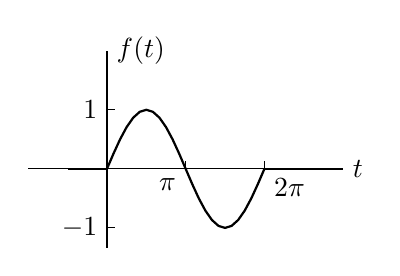
\begin{tikzpicture}
\draw(-1,0)--(3,0)node[right]{$t$};
\draw(0,-1)--(0,1.5)node[right]{$f(t)$};
\draw[thick](-0.5,0)--(0,0)(2,0)--(3,0);
\draw[thick,domain=0:360] plot ({2/360*\x},{0.75*sin(\x)});
\draw(0,-0.75)node[left]{$-1$}--++(0.1,0);
\draw(0,0.75)node[left]{$1$}--++(0.1,0);
\draw(1,0)node[below left]{$\pi$}--++(0,0.1);
\draw(2,0)node[below right]{$2\pi$}--++(0,0.1);
\end{tikzpicture}
\caption{تار کے بائیں سر کی حرکت (مثال \حوالہ{مثال_جزوی_نصف_لامتناہی_تار_لاپلاس})}
\label{شکل_مثال_جزوی_نصف_لامتناہی_تار_لاپلاس}
\end{figure}
ظاہر ہے کہ حقیقت میں لامتناہی تار نہیں پائی جاتی ہے لیکن یہ (قابل نظر انداز وزن کی) زیادہ لمبی تار جس کا دایاں سر \عددی{x} محور پر کسی دو نقطہ سے بندھا ہو کی نمونہ کشی کرتی ہے۔\\
حل:\quad ہمیں مساوات موج (حصہ \حوالہ{حصہ_جزوی_ارتعاش_تار})
\begin{align}\label{مساوات_نصف_لامتناہی_تار_مثال_الف}
\frac{\partial^{\,2}w}{\partial t^2}=c^2\frac{\partial^{\,2}w}{\partial x^2}\quad \quad \quad c^2=\frac{T}{\rho}
\end{align}
زیر سرحدی شرائط
\begin{align}\label{مساوات_نصف_لامتناہی_تار_مثال_ب}
w(0,t)=f(t),\quad \lim_{x\to\infty}=0\quad \quad \quad (t\ge 0)
\end{align}
اور ابتدائی شرائط 
\begin{align}
w(x,0)&=0\label{مساوات_نصف_لامتناہی_تار_مثال_پ}\\
\left.\frac{\partial w}{\partial t} \right|_{t=0}&=0\label{مساوات_نصف_لامتناہی_تار_مثال_ت}
\end{align}
 حل کرنی ہے۔ہم \عددی{t} کے لحاظ سے لاپلاس بدل لیتے ہیں۔یوں مساوات \حوالہ{مساوات_لاپلاس_درجہ_دوم_تفرق} کی مدد سے درج ذیل حاصل ہو گا۔
\begin{align*}
\Laplace(\frac{\partial^{\,2}w}{\partial t^2})=s^2\Laplace(w)-sw(x,0)-\left.\frac{\partial w}{\partial t}\right|_{t=0}=c^2\Laplace(\frac{\partial^{\,2}w}{\partial x^2})
\end{align*}
مساوات \حوالہ{مساوات_نصف_لامتناہی_تار_مثال_پ} اور مساوات \حوالہ{مساوات_نصف_لامتناہی_تار_مثال_ت} کی بنا دو اجزاء حذف ہوں گے۔دائیں ہاتھ ہم فرض کرتے ہیں کہ تکمل اور تفرق کی ترتیب بدلی جا سکتی ہے۔یوں
\begin{align*}
\Laplace(\frac{\partial^{\,2}w}{\partial x^2})=\int_0^{\infty} e^{-st}\frac{\partial^{\,2}w}{\partial x^2}\,\dif t=\frac{\partial^{\,2}}{\partial x^2}\int_0^{\infty}e^{-st}w(x,t)\,\dif t=\frac{\partial^{\,2}}{\partial x^2}\Laplace[w(x,t)]
\end{align*}
لکھا جا سکتا ہے جس میں \عددی{W(x,s)=\Laplace[w(x,t)]} لکھتے ہوئے
\begin{align*}
s^2W=c^2\frac{\partial^{\,2}W}{\partial x^2}
\end{align*}
یعنی
\begin{align*}
\frac{\partial^{\,2}W}{\partial x^2}-\frac{s^2}{c^2}W=0
\end{align*}
ملتا ہے۔چونکہ اس مساوات میں صرف \عددی{x} کے ساتھ تفرق پایا جاتا ہے لہٰذا اس کو سادہ تفرقی مساوات تصور کیا جاتا ہے جس کا نا معلوم تفاعل \عددی{W(x,s)} کے جو متغیرہ \عددی{x} کے تابع ہے۔اس کا عمومی حل
\begin{align}\label{مساوات_نصف_لامتناہی_تار_مثال_ٹ}
W(x,s)=A(s)e^{\frac{sx}{c}}+B(s)e^{-\frac{sx}{c}}
\end{align}
ہے۔مساوات \حوالہ{مساوات_نصف_لامتناہی_تار_مثال_ب} سے \عددی{F(s)=\Laplace[f(t)]} لکھتے ہوئے
\begin{align*}
W(0,s)=\Laplace[w(0,t)]=\Laplace[f(t)]=F(s)
\end{align*}
ملتا ہے۔اب فرض کریں کہ تکمل اور تفرق کی ترتیب دبلی جا سکتی ہے۔یوں
\begin{gather}
\begin{aligned}\label{مساوات_نصف_لامتناہی_تار_مثال_ث}
\lim_{x\to\infty} W(x,s)&=\lim_{x\to \infty}\int_0^{\infty}e^{-st}w(x,t)\,\dif t\\
&=\int_0^{\infty} e^{-st}\lim_{x\to \infty} w(x,t)\,\dif t=0
\end{aligned}
\end{gather}
 ہو گا۔ اب \عددی{c>0} ہے جبکہ مساوات \حوالہ{مساوات_نصف_لامتناہی_تار_مثال_ٹ} میں \عددی{s} کی کسی بھی مثبت قیمت کے لئے \عددی{x\to \infty} کرنے  سے  \عددی{e^{\tfrac{sx}{c}}\to \infty} ہو گا لہٰذا  مساوات \حوالہ{مساوات_نصف_لامتناہی_تار_مثال_ث} کے تحت  مساوات \حوالہ{مساوات_نصف_لامتناہی_تار_مثال_ٹ} میں \عددی{A(s)=0} ہو گا۔چونکہ کسی معین \عددی{\alpha} سے زیادہ کسی بھی \عددی{s} کے لئے لاپلاس بدل موجود (حصہ \حوالہ{حصہ_لاپلاس_تکملات_کا_بدل}) ہو گا لہٰذا ہم \عددی{s>0} فرض کر سکتے ہیں اور یوں
\begin{align*}
W(0,s)=B(s)=F(s)
\end{align*}
ہو گا۔اس طرح مساوات \حوالہ{مساوات_نصف_لامتناہی_تار_مثال_ٹ} سے درج ذیل ملتا ہے۔
\begin{align*}
W(x,s)=F(s)e^{-\frac{sx}{c}}
\end{align*}
منتقلی کا دوسرا مسئلہ  \حوالہ{مسئلہ_لاپلاس_وقتی_محور_منتقلی} میں \عددی{a=\tfrac{x}{c}} لیتے ہوئے الٹ لاپلاس بدل (شکل \حوالہ{شکل_مثال_جزوی_نصف_لامتناہی_تار_پر_حرکت}) 
\begin{align}\label{مساوات_نصف_لامتناہی_تار_مثال_ج}
w(x,t)=f\big(t-\frac{x}{c}\big)u_{\tfrac{x}{c}}(t)
\end{align}
یعنی
\begin{align}
w(x,t)=
\begin{cases}
\sin\big(t-\frac{x}{c}\big)& \frac{x}{c}<t<\frac{x}{c}+2\pi \quad \text{یا}\quad ct>x>(t-2\pi)c\\
0&\text{\RL{باقی اوقات}}
\end{cases}
\end{align}
حاصل کرتے ہیں جو رفتار \عددی{c} سے بائیں رخ حرکت کرتی واحد ایک موج  ہے۔یوں اگر موج بائیں سر سے لمحہ \عددی{t=0} پر روانہ ہو تب نقطہ \عددی{x}، لمحہ \عددی{t=\tfrac{x}{c}} تک ساکن رہتا ہے۔وقت \عددی{t=\tfrac{x}{c}} موج کو رفتار \عددی{c} پر چلتے ہوئے  فاصلہ \عددی{x} طے کرنے کے لئے درکار وقت ہے۔یہ تار یا رسی پر موج کی چال کی ہمارے مشاہدے کے عین مطابق ہے۔ آپ مساوات \حوالہ{مساوات_نصف_لامتناہی_تار_مثال_ج} کو مساوات \حوالہ{مساوات_نصف_لامتناہی_تار_مثال_الف} میں پر کرتے ہوئے تصدیق کر سکتے ہیں کہ یہی درست جواب ہے جو سرحدی اور ابتدائی شرائط کو مطمئن کرتا ہے۔
\begin{figure}
\centering
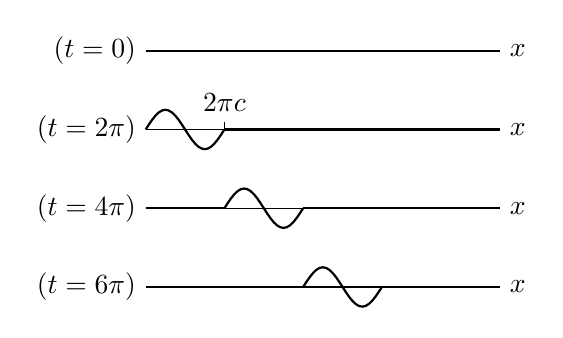
\begin{tikzpicture}
\pgfmathsetmacro{\k}{-1}
\draw(0,0)node[left]{$(t=0)$}--++(4.5,0)node[right]{$x$};
\draw(0,1*\k)node[left]{$(t=2\pi)$}--++(4.5,0)node[right]{$x$};
\draw(0,2*\k)node[left]{$(t=4\pi)$}--++(4.5,0)node[right]{$x$};
\draw(0,3*\k)node[left]{$(t=6\pi)$}--++(4.5,0)node[right]{$x$};
%
\draw[thick](0,0)--++(4.5,0);
\draw[thick,domain=0:360] plot ({\x/360},{1*\k+0.25*sin(\x)});
\draw(1,1*\k)--++(0,0.1)node[above]{$2\pi c$};
\draw[thick] (1,1*\k)--(4.5,1*\k);
\draw[thick,domain=0:360] plot ({1+\x/360},{2*\k+0.25*sin(\x)});
\draw[thick] (0,2*\k)--++(1,0);
\draw[thick](2,2*\k)--(4.5,2*\k);
\draw[thick,domain=0:360] plot ({2+\x/360},{3*\k+0.25*sin(\x)});
\draw[thick] (0,3*\k)--++(2,0);
\draw[thick](3,3*\k)--(4.5,3*\k);
\end{tikzpicture}
\caption{تار پر موج کی حرکت (مثال \حوالہ{مثال_جزوی_نصف_لامتناہی_تار_لاپلاس})}
\label{شکل_مثال_جزوی_نصف_لامتناہی_تار_پر_حرکت}
\end{figure}
\انتہا{مثال}
%========================

\حصہء{سوالات}

%================
\ابتدا{سوال}\quad
\عددی{c=1} اور تکونی \عددی{f} کی صورت میں  شکل \حوالہ{شکل_مثال_جزوی_نصف_لامتناہی_تار_پر_حرکت} کی طرح موج کی حرکت دکھائیں۔
\begin{align}
f(x)=
\begin{cases}
x&0<x<\frac{1}{2}\\
(l-x)&\frac{1}{2}<x<1
\end{cases}
\end{align}
\انتہا{سوال}
%=======================
\ابتدا{سوال}\quad
تار کی تناو اور کمیت کا مثال \حوالہ{مثال_جزوی_نصف_لامتناہی_تار_لاپلاس} میں موج کی رفتار پر کیا اثر ہو گا؟
\انتہا{سوال}
%======================
\ابتدا{سوال}\quad
مثال \حوالہ{مثال_جزوی_نصف_لامتناہی_تار_لاپلاس} میں حاصل کردہ حل کو مساوات موج میں پر کرتے ہوئے اس کی درستگی کی تصدیق کریں۔اگر ہم لمحہ \عددی{t=0} پر تار کی بائیں سر پر نا ختم ہونے والی سائن موج دیں تب نتائج کیا ہوں گے؟
\انتہا{سوال}
%===========================
لاپلاس بدل استعمال کرتے ہوئے سوال \حوالہ{سوال_جزوی_بذریعہ_لاپلاس_بدل_الف} تا سوال \حوالہ{سوال_جزوی_بذریعہ_لاپلاس_بدل_پ} حل کریں۔حاصل حل کو واپس دی گئی جزوی تفرقی مساوات میں پر کرتے ہوئے حل کی درستگی کی تصدیق کریں۔

%=================
\ابتدا{سوال}\شناخت{سوال_جزوی_بذریعہ_لاپلاس_بدل_الف}\quad
$\frac{\partial u}{\partial x}+2x\frac{\partial u}{\partial t}=2x,\quad u(x,0)=1,\quad u(0,t)=1$
\انتہا{سوال}
%=======================
\ابتدا{سوال}\شناخت{سوال_جزوی_بذریعہ_لاپلاس_بدل_ب}\quad
\begin{align*}
x\frac{\partial u}{\partial x}+\frac{\partial u}{\partial t}=xt,\quad \substack{u(x,0)=0,\quad x\ge 0\\ u(0,t)=0,\quad t\ge 0}
\end{align*}
جواب:\quad
\begin{align*}
U(x,s)&=\tfrac{c(s)}{x^s}+\tfrac{x}{s^2(s+1)},\quad U(0,s)=0,\quad c(s)=0,\\
u(x,t)&=x(t-1+e^{-t})
\end{align*}
\انتہا{سوال}
%========================
\ابتدا{سوال}\شناخت{سوال_جزوی_بذریعہ_لاپلاس_بدل_پ}\quad سوال \حوالہ{سوال_جزوی_بذریعہ_لاپلاس_بدل_ب} کو کسی دوسرے طریقہ سے حل کریں۔
\انتہا{سوال}
%=====================
نصف لامتناہی ، اطراف سے حاجز شدہ سلاخ \عددی{x} محور پر \عددی{x=0} تا \عددی{x=\infty} پڑی ہے۔سلاخ میں ابتدائی درجہ حرارت صفر ہے۔مزید تمام معین \عددی{t\ge 0}  کے لئے \عددی{x\to \infty} پر \عددی{w(x,t) \to 0} جبکہ \عددی{w(0,t)=f(t)} ہے۔سلاخ میں درجہ حرارت \عددی{w(x,t)} حاصل کرنے کے لئے درج ذیل اقدام کریں۔

%===============
\ابتدا{سوال}\شناخت{سوال_جزوی_نصف_لامتناہی_سلاخ_حرارت_الف}\quad
مسئلہ کا ریاضی نمونہ حاصل کریں۔اس نمونے کا لاپلاس بدل لے کر درج ذیل حاصل کریں۔
\begin{align*}
sW(x,s)&=c^2\frac{\partial^{\,2}W}{\partial x^2}\quad \quad \quad W=\Laplace(w)\\
W(x,s)&=F(s)e^{-\frac{\sqrt{s}x}{c}}\quad \quad \quad F=\Laplace(f)
\end{align*} 
\انتہا{سوال}
%=======================
\ابتدا{سوال}\شناخت{سوال_جزوی_نصف_لامتناہی_سلاخ_حرارت_ب}\quad
مسئلہ الجھاو کی اطلاق سوال \حوالہ{سوال_جزوی_نصف_لامتناہی_سلاخ_حرارت_الف} پر کرتے ہوئے درج ذیل حاصل کریں۔
\begin{align*}
w(x,t)=\frac{x}{2c\sqrt{\pi}}\int_0^t f(t-\tau) \tau^{-\frac{3}{2}} e^{-\frac{x^2}{4c^2\tau}}\,\dif \tau
\end{align*}
\انتہا{سوال}
%=========================
\ابتدا{سوال}\شناخت{سوال_جزوی_نصف_لامتناہی_سلاخ_حرارت_پ}\quad
فرض کریں کہ \عددی{w(0,t)=f(t)=u_0(t)} ہے (حصہ \حوالہ{حصہ_لاپلاس_محور_پر_منتقل_اور_اکائی_سیڑھی})۔ اس کے مطابقتی \عددی{w}، \عددی{W} اور \عددی{F} کو بالترتیب \عددی{w_0}، \عددی{W_0} اور \عددی{F_0} سے ظاہر کریں۔یوں دکھائیں کہ سوال \حوالہ{سوال_جزوی_نصف_لامتناہی_سلاخ_حرارت_ب} میں درج ذیل ہو گا
\begin{align*}
w_0(x,t)=\frac{x}{2c\sqrt{\pi}}\int_0^t \tau^{-\frac{3}{2}}e^{-\frac{x^2}{4c^2\tau}}\,\dif \tau=1-\erf\big(\frac{x}{2c\sqrt{t}}\big)
\end{align*}
جہاں تفاعل \عددی{\erf} کی تعریف حصہ \حوالہ{حصہ_جزوی_نصف_لامتناہی_سلاخ} کی سوالات میں دی گئی ہے۔\\
جواب:\quad
\عددی{\tfrac{x^2}{4c^2\tau}=z} لے کر \عددی{z} کے ساتھ تکمل لیں اور \عددی{\erf(\infty)=1} استعمال کریں۔
\انتہا{سوال}
%=====================
\ابتدا{سوال}\quad
دکھائیں کہ سوال \حوالہ{سوال_جزوی_نصف_لامتناہی_سلاخ_حرارت_پ} میں درج ذیل ہو گا
\begin{align*}
W_0(x,s)=\frac{1}{s}e^{-\frac{\sqrt{s}x}{x}}
\end{align*}
جو مسئلہ الجھاو کی اطلاق سے درج ذیل دیتی ہے۔
\begin{align*}
w(x,t)=\int_0^t f(t-\tau)\frac{\partial w_0}{\partial \tau}\,\dif \tau
\end{align*}
یہ کسی بھی تفاعل \عددی{f}  کا حل، تفاعل \عددی{f(t)=u_0(t)} کے حل \عددی{w_0} کی صورت میں دیتی ہے۔
\انتہا{سوال}
%=================
